%%%%%%%%%%%%%%%%%%%%%%% file template.tex %%%%%%%%%%%%%%%%%%%%%%%%%
%DIF LATEXDIFF DIFFERENCE FILE
%DIF DEL old_version.tex       Thu Dec 12 21:43:07 2019
%DIF ADD Gross-EPJP-2019.tex   Thu Dec 12 22:39:10 2019
%
% This is a template file for The European Physical Journal PLUS
%
% Copy it to a new file with a new name and use it as the basis
% for your article
%
%%%%%%%%%%%%%%%%%%%%%%%% Springer-Verlag / Societa` Italiana di Fisica  %%%%%%%%%%%%%%%%%%%%%%%%%
%
%\begin{filecontents}{leer.eps}
%!PS-Adobe-2.0 EPSF-2.0
%%%CreationDate: Mon Jul 13 16:51:17 1992
%%%DocumentFonts: (atend)
%%%Pages: 0 1
%%%BoundingBox: 72 31 601 342
%%%EndComments
%
%gsave
%72 31 moveto
%72 342 lineto
%601 342 lineto
%601 31 lineto
%72 31 lineto
%showpage
%grestore
%%%Trailer
%%%DocumentFonts: Helvetica
%\end{filecontents}
%
\documentclass[epj]{svjour}
% Remove option referee for final version
%
% Remove any % below to load the required packages
%\usepackage{latexsym}
\usepackage{mathtools} % Loads amsmath
\usepackage{graphics}
\usepackage{amsmath}
\usepackage{amssymb}
\usepackage{latexsym}
\usepackage{amsfonts}
\usepackage{authblk}
\usepackage{xfrac}
\usepackage{graphicx}
%\usepackage[colorlinks=true,linkcolor=black, citecolor=blue, urlcolor=blue]{hyperref} % for hyperrefs
%\usepackage{cleveref}
%\usepackage[authoryear]{natbib}
\usepackage{gensymb}  % provides macro \degree which works in text and math
\usepackage{color}
%\usepackage{enumitem} 
\usepackage{bm}
\usepackage{multirow}
\usepackage{cite}
%DIF 53a53-56
\usepackage{subcaption} % For subfigure %DIF > 
\captionsetup{compatibility=false} %DIF > 
\usepackage{wrapfig} %DIF > 
%\usepackage{caption} % Caption in subfigure %DIF > 
%DIF -------
\usepackage{tikz}
\usetikzlibrary{arrows}

% for quotes
%DIF 57-59c61-63
%DIF < \usepackage [english]{babel}
%DIF < \usepackage [autostyle, english = american]{csquotes}
%DIF < \MakeOuterQuote{"}
%DIF -------
% \usepackage [english]{babel} %DIF > 
% \usepackage [autostyle, english = american]{csquotes} %DIF > 
% \MakeOuterQuote{"} %DIF > 
%DIF -------

% for flow charts
% Define block styles
%DIF 63c67-68
%DIF < \usepackage{tikz}
%DIF -------
 %DIF > 
\usetikzlibrary{patterns} %DIF > 
%DIF -------
\usetikzlibrary{shapes,arrows}
\tikzstyle{discre} = [rectangle, draw, fill=white!20, 
text width=6em, text centered, minimum height=3em, node distance=3.5cm, line width=1pt]
\tikzstyle{decision} = [diamond, draw, fill=white!20, 
%DIF 68c73
%DIF < text width=3em, text badly centered, node distance=2cm, inner sep=1pt, line width=1pt]
%DIF -------
text width=4em, text badly centered, node distance=2cm, inner sep=2pt, line width=1pt] %DIF > 
%DIF -------
\tikzstyle{block} = [rectangle, draw, fill=white!20, 
text width=6em, text centered, minimum height=3em, node distance=3.5cm, line width=1pt]
\tikzstyle{blockEq} = [rectangle, draw, fill=white!20, 
text width=8em, text centered, minimum height=3em, node distance=3.5cm, line width=0pt]
\tikzstyle{cloud} = [draw, ellipse,fill=white!20, node distance=4cm,
text centered, text width=3em, minimum height=2em, line width=1pt]
\tikzstyle{line} = [draw, -{latex'}, line width=1.0pt]

% For merging cells 
\usepackage{array}
\usepackage{booktabs}
\setlength{\heavyrulewidth}{1.5pt}
\setlength{\abovetopsep}{4pt}

%DIF 83d88
%DIF < 
%DIF -------
% etc
%

\newcommand{\eq}[1]{Eq.~(\ref{#1})}
\newcommand{\eqnolabel}[1]{(\ref{#1})}
\newcommand{\eqs}[1]{Eqs.~(\ref{#1})}
\newcommand{\eqsthru}[2]{Eqs.~(\ref{#1})--(\ref{#2})}
\newcommand{\eqsand}[2]{Eqs.~(\ref{#1}) and (\ref{#2})}
\newcommand{\tbl}[1]{Table~\ref{#1}}
\newcommand{\tblnolabel}[1]{\ref{#1}}
\newcommand{\tbls}[1]{Tables~\ref{#1}}
\newcommand{\tblsthru}[2]{Tables~\ref{#1}--\ref{#2}}
\newcommand{\tblsand}[2]{Tables~\ref{#1} and \ref{#2}}
\newcommand{\fig}[1]{Fig.~\ref{#1}}
\newcommand{\fignolabel}[1]{\ref{#1}}
\newcommand{\figs}[1]{Figs.~\ref{#1}}
\newcommand{\figsthru}[2]{Figs.~\ref{#1}--\ref{#2}}
\newcommand{\figsand}[2]{Figs.~\ref{#1} and \ref{#2}}
\newcommand{\sxn}[1]{Section~\ref{#1}}

\newcommand{\revised}[1]{{\color{red}{#1}}}
\newcommand{\tsup}[1]{\textsuperscript{#1}}
\newcommand{\tsub}[1]{\textsubscript{#1}}

\newcommand{\erez}[1]{{\color{blue}{\textsuperscript{EREZ:}#1}}}
\newcommand{\roy}[1]{{\color{blue}{\textsuperscript{ROY:}#1}}}

\newcommand{\keff}{{\ensuremath{k_{\textrm{\scriptsize{eff}}}}}}
%DIF 112a116-118
\newcommand{\kref}{{\ensuremath{k_{\textrm{\scriptsize{ref}}}}}} %DIF > 
\newcommand{\krm}{{\ensuremath{k_{\textrm{\scriptsize{RM}}}}}} %DIF > 
\newcommand{\kd}{{\ensuremath{k_{\textrm{\scriptsize{D}}}}}} %DIF > 
%DIF -------
\newcommand{\beff}{\ensuremath{\beta_{\textrm{eff}}}}
\newcommand{\rr}{\ensuremath{\bm{r}}}
\newcommand{\OO}{\ensuremath{\hat{\bm{\Omega}}}}
\newcommand{\bnabla}{\ensuremath{\bm{\nabla}}}
\newcommand{\rE}{\ensuremath{(\rr,E)}}

\newcommand{\ftr}{\ensuremath{\phi_{\textrm{\scriptsize{tr}}}}}
\newcommand{\jtr}{\ensuremath{\bm{J}_{\textrm{\scriptsize{tr}}}}}
\newcommand{\jtrr}{\ensuremath{J_{\textrm{\scriptsize{tr}}}}}
%DIF 121a128-129
\newcommand{\jd}{\ensuremath{J_{\textrm{\scriptsize{D}}}}} %DIF > 
\newcommand{\delj}{\ensuremath{\delta J}} %DIF > 
%DIF -------
%\newcommand{\mcL}{\mathcal{L}}
\newcommand{\mcL}{\tau}
\newcommand{\pl}[1]{\ensuremath{P_l(#1)}}
\newcommand{\dx}{\ensuremath{\Delta x}}

%
\graphicspath{ {./figures/} }
% ---------------------------------------------------
%DIF PREAMBLE EXTENSION ADDED BY LATEXDIFF
%DIF UNDERLINE PREAMBLE %DIF PREAMBLE
\RequirePackage[normalem]{ulem} %DIF PREAMBLE
\RequirePackage{color}\definecolor{RED}{rgb}{1,0,0}\definecolor{BLUE}{rgb}{0,0,1} %DIF PREAMBLE
\providecommand{\DIFadd}[1]{{\protect\color{blue}\uwave{#1}}} %DIF PREAMBLE
\providecommand{\DIFdel}[1]{{\protect\color{red}\sout{#1}}}                      %DIF PREAMBLE
%DIF SAFE PREAMBLE %DIF PREAMBLE
\providecommand{\DIFaddbegin}{} %DIF PREAMBLE
\providecommand{\DIFaddend}{} %DIF PREAMBLE
\providecommand{\DIFdelbegin}{} %DIF PREAMBLE
\providecommand{\DIFdelend}{} %DIF PREAMBLE
\providecommand{\DIFmodbegin}{} %DIF PREAMBLE
\providecommand{\DIFmodend}{} %DIF PREAMBLE
%DIF FLOATSAFE PREAMBLE %DIF PREAMBLE
\providecommand{\DIFaddFL}[1]{\DIFadd{#1}} %DIF PREAMBLE
\providecommand{\DIFdelFL}[1]{\DIFdel{#1}} %DIF PREAMBLE
\providecommand{\DIFaddbeginFL}{} %DIF PREAMBLE
\providecommand{\DIFaddendFL}{} %DIF PREAMBLE
\providecommand{\DIFdelbeginFL}{} %DIF PREAMBLE
\providecommand{\DIFdelendFL}{} %DIF PREAMBLE
\newcommand{\DIFscaledelfig}{0.5}
%DIF HIGHLIGHTGRAPHICS PREAMBLE %DIF PREAMBLE
\RequirePackage{settobox} %DIF PREAMBLE
\RequirePackage{letltxmacro} %DIF PREAMBLE
\newsavebox{\DIFdelgraphicsbox} %DIF PREAMBLE
\newlength{\DIFdelgraphicswidth} %DIF PREAMBLE
\newlength{\DIFdelgraphicsheight} %DIF PREAMBLE
% store original definition of \includegraphics %DIF PREAMBLE
\LetLtxMacro{\DIFOincludegraphics}{\includegraphics} %DIF PREAMBLE
\newcommand{\DIFaddincludegraphics}[2][]{{\color{blue}\fbox{\DIFOincludegraphics[#1]{#2}}}} %DIF PREAMBLE
\newcommand{\DIFdelincludegraphics}[2][]{% %DIF PREAMBLE
\sbox{\DIFdelgraphicsbox}{\DIFOincludegraphics[#1]{#2}}% %DIF PREAMBLE
\settoboxwidth{\DIFdelgraphicswidth}{\DIFdelgraphicsbox} %DIF PREAMBLE
\settoboxtotalheight{\DIFdelgraphicsheight}{\DIFdelgraphicsbox} %DIF PREAMBLE
\scalebox{\DIFscaledelfig}{% %DIF PREAMBLE
\parbox[b]{\DIFdelgraphicswidth}{\usebox{\DIFdelgraphicsbox}\\[-\baselineskip] \rule{\DIFdelgraphicswidth}{0em}}\llap{\resizebox{\DIFdelgraphicswidth}{\DIFdelgraphicsheight}{% %DIF PREAMBLE
\setlength{\unitlength}{\DIFdelgraphicswidth}% %DIF PREAMBLE
\begin{picture}(1,1)% %DIF PREAMBLE
\thicklines\linethickness{2pt} %DIF PREAMBLE
{\color[rgb]{1,0,0}\put(0,0){\framebox(1,1){}}}% %DIF PREAMBLE
{\color[rgb]{1,0,0}\put(0,0){\line( 1,1){1}}}% %DIF PREAMBLE
{\color[rgb]{1,0,0}\put(0,1){\line(1,-1){1}}}% %DIF PREAMBLE
\end{picture}% %DIF PREAMBLE
}\hspace*{3pt}}} %DIF PREAMBLE
} %DIF PREAMBLE
\LetLtxMacro{\DIFOaddbegin}{\DIFaddbegin} %DIF PREAMBLE
\LetLtxMacro{\DIFOaddend}{\DIFaddend} %DIF PREAMBLE
\LetLtxMacro{\DIFOdelbegin}{\DIFdelbegin} %DIF PREAMBLE
\LetLtxMacro{\DIFOdelend}{\DIFdelend} %DIF PREAMBLE
\DeclareRobustCommand{\DIFaddbegin}{\DIFOaddbegin \let\includegraphics\DIFaddincludegraphics} %DIF PREAMBLE
\DeclareRobustCommand{\DIFaddend}{\DIFOaddend \let\includegraphics\DIFOincludegraphics} %DIF PREAMBLE
\DeclareRobustCommand{\DIFdelbegin}{\DIFOdelbegin \let\includegraphics\DIFdelincludegraphics} %DIF PREAMBLE
\DeclareRobustCommand{\DIFdelend}{\DIFOaddend \let\includegraphics\DIFOincludegraphics} %DIF PREAMBLE
\LetLtxMacro{\DIFOaddbeginFL}{\DIFaddbeginFL} %DIF PREAMBLE
\LetLtxMacro{\DIFOaddendFL}{\DIFaddendFL} %DIF PREAMBLE
\LetLtxMacro{\DIFOdelbeginFL}{\DIFdelbeginFL} %DIF PREAMBLE
\LetLtxMacro{\DIFOdelendFL}{\DIFdelendFL} %DIF PREAMBLE
\DeclareRobustCommand{\DIFaddbeginFL}{\DIFOaddbeginFL \let\includegraphics\DIFaddincludegraphics} %DIF PREAMBLE
\DeclareRobustCommand{\DIFaddendFL}{\DIFOaddendFL \let\includegraphics\DIFOincludegraphics} %DIF PREAMBLE
\DeclareRobustCommand{\DIFdelbeginFL}{\DIFOdelbeginFL \let\includegraphics\DIFdelincludegraphics} %DIF PREAMBLE
\DeclareRobustCommand{\DIFdelendFL}{\DIFOaddendFL \let\includegraphics\DIFOincludegraphics} %DIF PREAMBLE
%DIF LISTINGS PREAMBLE %DIF PREAMBLE
\RequirePackage{listings} %DIF PREAMBLE
\RequirePackage{color} %DIF PREAMBLE
\lstdefinelanguage{DIFcode}{ %DIF PREAMBLE
%DIF DIFCODE_UNDERLINE %DIF PREAMBLE
  moredelim=[il][\color{red}\sout]{\%DIF\ <\ }, %DIF PREAMBLE
  moredelim=[il][\color{blue}\uwave]{\%DIF\ >\ } %DIF PREAMBLE
} %DIF PREAMBLE
\lstdefinestyle{DIFverbatimstyle}{ %DIF PREAMBLE
	language=DIFcode, %DIF PREAMBLE
	basicstyle=\ttfamily, %DIF PREAMBLE
	columns=fullflexible, %DIF PREAMBLE
	keepspaces=true %DIF PREAMBLE
} %DIF PREAMBLE
\lstnewenvironment{DIFverbatim}{\lstset{style=DIFverbatimstyle}}{} %DIF PREAMBLE
\lstnewenvironment{DIFverbatim*}{\lstset{style=DIFverbatimstyle,showspaces=true}}{} %DIF PREAMBLE
%DIF END PREAMBLE EXTENSION ADDED BY LATEXDIFF

\begin{document}
%
\title{High-accuracy neutron diffusion calculations based on integral transport theory}
%\subtitle{}
\author{
	Roy Gross\inst{1} \and 
	Daniele Tomatis\inst{2} \and 
	Erez Gilad\inst{1}\thanks{\email{gilade@bgu.ac.il} (corresponding author)}
}                     % Do not remove
%
%\offprints{}          % Insert a name or remove this line
%
\institute{
	The Unit of Nuclear Engineering, Ben-Gurion University of the Negev, 8410501 Beer-Sheva, Israel 
	\and
	CEA, DEN, Service d'{\'e}tudes des r\'eacteurs et de math\'ematiques appliqu\'ees (SERMA),\DIFaddbegin \\
	\DIFaddend Universit\'e Paris-Saclay, F-91191 Gif-sur-Yvette, France}
%
\authorrunning{Gross, Tomatis \& Gilad} 
\titlerunning{Integral transport correction to diffusion calculations}
\date{Received: date / Revised version: date}
% The correct dates will be entered by Springer
%
\abstract{
In this paper, the Ronen method is developed, implemented\DIFaddbegin \DIFadd{, }\DIFaddend and applied to resolve the neutron flux and the criticality eigenvalue in \DIFdelbegin \DIFdel{a }\DIFdelend simple \DIFaddbegin \DIFadd{one-dimensional }\DIFaddend homogeneous \DIFdelbegin \DIFdel{problem}\DIFdelend \DIFaddbegin \DIFadd{and heterogeneous problems}\DIFaddend . The Ronen method is based on iterative calculations of \DIFdelbegin \DIFdel{the multigroup diffusion coefficients using }\DIFdelend \DIFaddbegin \DIFadd{correction factors to use in }\DIFaddend a multigroup diffusion model\DIFdelbegin \DIFdel{and driven }\DIFdelend \DIFaddbegin \DIFadd{, where the factors are actually given }\DIFaddend by the \DIFdelbegin \DIFdel{solutions of the }\DIFdelend integral transport equation. \DIFdelbegin \DIFdel{The local }\DIFdelend \DIFaddbegin \DIFadd{In particular, spatially-dependent }\DIFaddend diffusion constants are modified \DIFaddbegin \DIFadd{locally }\DIFaddend in order to reproduce new estimates of the surface currents \DIFaddbegin \DIFadd{obtained }\DIFaddend by \DIFdelbegin \DIFdel{a }\DIFdelend \DIFaddbegin \DIFadd{the integral }\DIFaddend transport operator. The diffusion solver employed in this study uses finite differences and the transport-corrected currents are introduced into the numerical scheme \DIFdelbegin \DIFdel{by means of }\DIFdelend \DIFaddbegin \DIFadd{as }\DIFaddend drift terms. The corrected solutions are compared against reference results \DIFdelbegin \DIFdel{obtained  by }\DIFdelend \DIFaddbegin \DIFadd{from }\DIFaddend a discrete ordinate code. \DIFdelbegin \DIFdel{Boundary conditions are discussed and proper approximations are introduced in order to conserve the particle balance. }\DIFdelend %DIF > Boundary conditions are discussed and proper approximations are introduced to conserve the particle balance.  %% commented because this is treated in another article indeed.
The results match \DIFdelbegin \DIFdel{extremely }\DIFdelend well \DIFaddbegin \DIFadd{with }\DIFaddend the reference solutions, especially in the limit of fine meshes, but slow convergence of the scalar flux is reported.
% 
\PACS{
	{28.00.00}{Nuclear engineering and nuclear power studies} \and
	{28.20.Gd}{Neutron transport: diffusion and moderation} \and
	{05.60.-k}{Transport processes} \and
	{28.41.-i}{Fission reactors}
     } % end of PACS codes
  \keywords{
  	neutron diffusion -- integral transport -- non-linear transport correction
  }
} %end of abstract
%
\maketitle
%
% ---------------------------------------------------
\section{Introduction}
\label{sec:intro}

Neutron transport calculations on a full core scale can be a highly intensive computational task. High-fidelity core design optimization or transient analyses can quickly become computationally impractical when using transport methods~\cite{Kim-2019}. For example, \DIFdelbegin \DIFdel{in order }\DIFdelend \DIFaddbegin \DIFadd{about 10\tsup{11} histories are needed in a full-core Monte Carlo calculation }\DIFaddend to achieve a 1\% accuracy \DIFdelbegin \DIFdel{in the }\DIFdelend \DIFaddbegin \DIFadd{on }\DIFaddend local flux/power estimation\DIFdelbegin \DIFdel{, an order of 10\tsup{11} histories is needed in a full-core Monte Carlo calculation}\DIFdelend ~\cite{Martin-2012}. Another problem is the huge number of variables and parameters to be stored and used during computation, e.g., tallies, geometry, cross sections, and depletion data. A conservative estimation of the memory needed for reasonably accurate full-core Monte Carlo neutronic calculation is in the range of terabytes (TBs)~\cite{Martin-2012}. \DIFaddbegin \DIFadd{The growing demand for high-accuracy and high-precision full-core computations challenges not only today’s high-end computing systems but will also challenge the near future (e.g., Exascale) computers~\mbox{%DIFAUXCMD
\cite{Martin-2012,Smith-2011,Kim-2019}}\hspace{0pt}%DIFAUXCMD
.  
}\DIFaddend 

%DIF < The growing demand for high-accuracy and high-precision full-core computations challenges not only today’s high-end computing systems but will also challenge the near future (e.g., Exascale) computers~\cite{Martin-2012,Smith-2011,Kim-2019}.  
\DIFdelbegin %DIFDELCMD < 

%DIFDELCMD < %%%
\DIFdelend To overcome this difficulty, faster (and less accurate) multigroup neutron diffusion solvers are frequently used~\cite{Lawrence-1986,Smith-1986}. However, future Gen-IV reactor designs are characterized by strong heterogeneity in the core, e.g., axial and radial seed-blanket structures, as in the French ASTRID SFR CVF design~\cite{Bertrand-2016}, challenging the accuracy of diffusion calculations. Moreover, modern calculation schemes evolve towards so-called \DIFdelbegin \DIFdel{"}\DIFdelend \DIFaddbegin \DIFadd{``}\DIFaddend best-estimate\DIFdelbegin \DIFdel{" }\DIFdelend \DIFaddbegin \DIFadd{'' }\DIFaddend codes, aiming at high accuracy~\cite{IAEA-BE-2008}. 

A crucial issue in obtaining an accurate diffusion calculation is the formulation of the diffusion coefficient~\cite{Bell-1970,Pounders-2009}. The calculation of this parameter should be based on physical insights from the transport equation\DIFaddbegin \DIFadd{, }\DIFaddend such that the resulting \DIFdelbegin \DIFdel{improved ("transport corrected") }\DIFdelend diffusion approximation can \DIFaddbegin \DIFadd{really }\DIFaddend capture the transport phenomena of interest. \DIFdelbegin \DIFdel{Such }\DIFdelend \DIFaddbegin \DIFadd{Improved diffusion models obtained through }\DIFaddend transport corrections can be divided into two main classes. The first class is based on extending the $P_1$ model equations (and the associated boundary conditions) along with some closure scheme, such as the well-known $SP_3$ approximation~\cite{Brantley-2000}. The second class, to which this study belongs, is based on the re-calculation of \DIFdelbegin \DIFdel{the diffusion coefficients }\DIFdelend \DIFaddbegin \DIFadd{correction factors }\DIFaddend within the multigroup diffusion framework~\cite{Tomatis-2011}. 

In this paper, the development, implementation, and qualification of the Ronen Method~\cite{Ronen-2004} in one-dimensional homogeneous \DIFaddbegin \DIFadd{and heterogeneous }\DIFaddend plane geometry is reported. This method is implemented as a highly accurate multigroup neutron diffusion solver based on novel transport corrections. The main hypothesis underlying the Ronen method is based on iterative calculations of the multigroup diffusion coefficients driven by the solutions of the integral transport equation~\cite{Ronen-2004,Tomatis-2011}. 

%This study addresses a critical issue in contemporary nuclear reactor calculations, which constitutes an inherent difficulty that will not be solved in the near future merely by increased computational capabilities. As modern and advanced nuclear systems become more complex and heterogeneous, the requirements for more precise and accurate calculations increase as well~\cite{Smith-2011,Martin-2012,Smith-2013,Tomatis-2011,Kim-2019}. This trend is not likely to fade away. In light of this trend, the development of highly accurate neutron diffusion calculations is of great importance for nuclear reactor's operation, safety, research, and design purposes.

The theoretical background is detailed in~\sxn{sec:theory}, the numerical implementation is described in~\sxn{sec:imp}, the results are presented in~\sxn{sec:res}\DIFaddbegin \DIFadd{, }\DIFaddend and conclusions are brought in~\sxn{sec:conc}.

%
% ---------------------------------------------------
\section{Theoretical background}
\label{sec:theory}

%
% ---------------------------------------------------
\subsection{The Ronen method}
\label{sec:RM}

In 2004, Ronen~\cite{Ronen-2004} suggested to derive corrected diffusion coefficients using Fick's law and more accurate estimations of the neutron currents by means of integral transport operators, whereas the neutron flux is resolved by diffusion theory. Denoting the \DIFdelbegin \DIFdel{integral transport and diffusion currentsby }\DIFdelend \DIFaddbegin \DIFadd{currents obtained by integral transport as ``integral currents'' }\DIFaddend $\jtr\rE$ and \DIFaddbegin \DIFadd{the currents obtained by Fick's law as ``diffusion currents'' }\DIFaddend $\bm{J}_D\rE$, \DIFdelbegin \DIFdel{respectively, }\DIFdelend the Ronen idea is based on changing the diffusion coefficient such that
\begin{equation}\label{eq:Fick}
\bm{J}_D\rE = -D\rE\bnabla\phi\rE = \jtr\rE\DIFdelbegin \DIFdel{\,\, }\DIFdelend . 
\end{equation}

Since these accurate estimates of the currents are based on a known flux distribution, it was also suggested to execute new diffusion calculations, thus updating iteratively the diffusion coefficients in the global calculation. 
\begin{equation}\label{eq:RM-it}
D^{(k+1)}\rE = -\DIFdelbegin \DIFdel{\frac{\jtr^{(k)}\rE}{\bnabla\phi^{(k)}\rE} \,\, }\DIFdelend \DIFaddbegin \DIFadd{\frac{\lvert\jtr^{(k)}\rE\rvert}{\lvert\bnabla\phi^{(k)}\rE\rvert} }\DIFaddend ,
\end{equation}
where $k$ is the iteration index. \DIFaddbegin \DIFadd{The use of a tensor notation is needed for the diffusion coefficient in general multidimensional problems.
}\DIFaddend 

The motivation for this method was to overcome the inherent limitation of Fick's law requiring smooth flux gradients and thus small neutron absorption rate with respect to scattering in general. Nevertheless, isotropic scattering remained as a basic postulate.
For example, in a \DIFdelbegin \DIFdel{one-dimensional }\DIFdelend homogeneous slab with void boundary conditions, Eq.~\eqref{eq:RM-it} takes the following form~\cite{Ronen-2004} 
\begin{equation}\label{eq:RM-it-1D-slab}
D^{(k+1)}(x,E) = -\DIFdelbegin \DIFdel{\frac{\frac{1}{2}\int_0^a dx' E_2[\sigma(E)\lvert
	x-x'\rvert]\text{sign}(x-x')q^{(k)}(x',E)}{\partial \phi^{(k)}(x,E)/\partial x} \,\, }\DIFdelend \DIFaddbegin \DIFadd{\frac{\displaystyle \frac{1}{2}\int_0^a dx' E_2[\sigma(E)\lvert
	x-x'\rvert]\operatorname{Sgn}(x-x')q^{(k)}(x',E)}{\partial \phi^{(k)}(x,E)/\partial x}}\DIFaddend .
\end{equation}

This idea was later used by Tomatis and Dall'Osso~\cite{Tomatis-2011}, who provided a numerical demonstration in a simple slab problem. Instead of updating the diffusion coefficient by the ratio of the current and the flux gradient, as in Fick's law, they adopted the Coarse Mesh Finite Differences method (CMFD) for taking into account \DIFdelbegin \DIFdel{the }\DIFdelend \DIFaddbegin \DIFadd{in the diffusion solver the }\DIFaddend new currents estimated by the integral transport operator\DIFdelbegin \DIFdel{in the diffusion solver}\DIFdelend . 
%
%They proposed to update non-linearly the diffusion coefficients at the cell interfaces of the spatial mesh by the coarse mesh finite differences method (CMFD).
%
This technique, largely adopted in the literature of nodal methods~\cite{Smith-1983,Lawrence-1986}, can avoid indeterminate divisions in case of vanishing flux gradients. They tested this implementation in a homogeneous bare slab using two-group cross sections representative of a realistic PWR assembly. It was observed that the Ronen method (RM) could drive the flux distribution away from diffusion and closer to the reference solution of the integral Boltzmann transport equation, regardless of the initial formulation used for the diffusion coefficient. As expected, the largest errors were located near the boundary \DIFdelbegin \DIFdel{, }\DIFdelend where the transport effects are \DIFdelbegin \DIFdel{most pronounced, }\DIFdelend \DIFaddbegin \DIFadd{more pronounced, but }\DIFaddend slowly decreasing even after many iterations.% Their work was limited to the homogeneous slab, and resolved neutron diffusion on the same discretized spatial mesh used for the reference from neutron transport.

%
% ---------------------------------------------------
\subsection{The one-dimensional Peierls equation}
\label{sec:Peierls}

There are several ways to \DIFdelbegin \DIFdel{drive }\DIFdelend \DIFaddbegin \DIFadd{derive }\DIFaddend the integral expression for the flux in slab geometry. Most of them start with assuming homogeneous and isotropic scattering and sources, yielding the \emph{Peierls equation} \cite{Davison-1957,Case-1967,Bell-1970,Pomraning-1973,Duderstadt-1979,Lewis-1984}. The derivation of expression for slab geometry (of thickness $a$) is straightforward, yielding
\begin{equation}\label{eq:flux-slab-l-0-no-bndry-terms}
\DIFdelbegin %DIFDELCMD < \begin{split}
%DIFDELCMD < \phi(x,E)=&\frac{1}{2}\int_0^a { dx'
%DIFDELCMD < 	E_1\left[\sigma(E)\lvert x-x'\rvert\right] q(x',E)
%DIFDELCMD < } \text{, with} \\
%DIFDELCMD < q(x',E) =& \int_0^\infty { dE'
%DIFDELCMD < 		\sigma_s(E \leftarrow E')\phi(x',E') + S(x',E)
%DIFDELCMD < }
%DIFDELCMD < \end{split}%%%
\DIFdelend \DIFaddbegin \begin{split}
\phi(x,E)=&\frac{1}{2}\int_0^a { dx'
	E_1\left[\sigma(E)\lvert x-x'\rvert\right] Q(x',E)
}, \text{ with} \\
Q(x,E) =& \int_0^\infty { dE'
		\sigma_s(E \leftarrow E')\phi(x,E') + S(x,E)
}
\end{split}\DIFaddend 
\end{equation}
%DIF <  commented to overcome an error of latexdiff
%DIF < \begin{eqnarray}\label{eq:flux-slab-l-0-no-bndry-terms}
%DIF < \phi(x,E)&=&\frac{1}{2}\int_0^a { dx'
%DIF < 	E_1\left[\sigma(E)\lvert x-x'\rvert\right] q(x',E) 
%DIF < }\nonumber \\
%DIF < &=& \frac{1}{2}\int_0^a { \!\!\! dx'
%DIF < 	E_1\left[\sigma(E)\lvert x-x'\rvert\right]
%DIF < 	\left[
%DIF < 	\int_0^\infty { \!\!\! dE'
%DIF < 		\sigma_s(E\leftarrow E')\phi(x',E') 
%DIF < 	} + S(x',E)
%DIF < 	\right] 
%DIF < } \,\, ,
%DIF < \end{eqnarray}
\DIFdelbegin \DIFdel{where }\DIFdelend \DIFaddbegin \DIFadd{and }\DIFaddend $E_1(x)$ \DIFdelbegin \DIFdel{is a }\DIFdelend \DIFaddbegin \DIFadd{as }\DIFaddend first order exponential integral~\cite{Abramowitz-1964}. Note that this expression does not include the contribution of uncollided neutrons \DIFdelbegin \DIFdel{originate from the }\DIFdelend \DIFaddbegin \DIFadd{originated from an incoming angular }\DIFaddend flux at the boundaries.

\DIFdelbegin \DIFdel{Another }\DIFdelend \DIFaddbegin \DIFadd{The }\DIFaddend starting point for the derivation of the integral expression for the flux in slab geometry is to directly integrate along a line the transport equation~\cite{Davison-1957,Pomraning-1973,Duderstadt-1979,Lewis-1984}
\begin{equation}\label{eq:full-ITE-w-bndry-terms}
\psi(\rr,\OO) = \int_0^R { dR'
	\DIFdelbegin \DIFdel{q}\DIFdelend \DIFaddbegin \DIFadd{Q}\DIFaddend (\rr-R'\OO,\OO) e^{-\mcL(\rr,\rr-R'\OO)}
} + \psi(\rr-R\OO,\OO) e^{-\mcL(\rr,\rr-R\OO)},
\end{equation}
%DIF <  commented to avoid an error by latexdiff
%DIF < \begin{eqnarray}\label{eq:full-ITE-w-bndry-terms}
%DIF < \psi(\rr,\OO) &=& \int_0^R { dR'
%DIF < 	q(\rr-R'\OO,\OO) e^{-\mcL(\rr,\rr-R'\OO)}
%DIF < } 
%DIF < %\nonumber \\
%DIF < %&+& 
%DIF < +\psi(\rr-R\OO,\OO) e^{-\mcL(\rr,\rr-R\OO)}
%DIF < \,\, ,
%DIF < \end{eqnarray}
where $\mcL(\rr,\rr-R'\OO)$ is the \emph{optical length}, defined as
\begin{equation}\label{eq:opl}
\mcL(\rr,\rr-R'\OO) \equiv \int_0^{R'} {\sigma(\rr-R''\OO)dR'} \DIFdelbegin \DIFdel{\,\, }\DIFdelend .
\end{equation}
Assuming isotropic scattering and homogeneous medium in one-dimension for~\eq{eq:full-ITE-w-bndry-terms} recovers~\eq{eq:flux-slab-l-0-no-bndry-terms}. 

In what follows, a generalization of~\eq{eq:flux-slab-l-0-no-bndry-terms} is derived for heterogeneous medium with anisotropic scattering.  
%
% ---------------------------------------------------
\subsection{Integral expressions for the neutron flux \DIFdelbegin \DIFdel{\& }\DIFdelend \DIFaddbegin \DIFadd{and }\DIFaddend current}
\label{sec:int-flux-J}

Consider an infinite \DIFdelbegin \DIFdel{one-dimensional }\DIFdelend slab of width $a$. The angular flux in the slab is given by~\cite{Lewis-1984}
\begin{subequations}\label{eq:int-ang-flx}
  \begin{eqnarray}
  \psi(x,E,\mu) &=& \psi(0,E,\mu) e^{-\mcL(0,x,E)/\mu}
  + \int_0^x { dx'
          \DIFdelbegin \DIFdel{\,\,
		}\DIFdelend \frac{Q(x',E,\mu)}{\mu} 
          e^{-\mcL(x',x,E)/\mu} 
  } \DIFdelbegin \DIFdel{\,\, }\DIFdelend , \qquad \mu>0 \DIFdelbegin \DIFdel{\,\, }\DIFdelend ,   \label{eq:int-ang-flx-a}\\
  \psi(x,E,\mu) &=& \psi(a,E,\mu)e^{\mcL(x,a,E)/\mu} 
  -\int_x^a { dx'
          \DIFdelbegin \DIFdel{\,\,
		}\DIFdelend \frac{Q(x',E,\mu)}{\mu} 
          e^{\mcL(x,x',E)/\mu} 
  } \DIFdelbegin \DIFdel{\,\, }\DIFdelend , \qquad \mu<0 \DIFdelbegin \DIFdel{\,\, }\DIFdelend , \label{eq:int-ang-flx-b}
  \end{eqnarray}
\end{subequations}
where
\begin{equation}\label{eq:opl2}
\mcL(x',x,E) \equiv \DIFaddbegin \operatorname{Sgn}\DIFadd{(x-x') }\DIFaddend \int_{x'}^x {\sigma(x'',E) dx''}
\DIFdelbegin \DIFdel{\,\, 
}\DIFdelend \end{equation}
and $Q(x,E,\mu)$ denotes \DIFdelbegin \DIFdel{all sources}\DIFdelend \DIFaddbegin \DIFadd{total emission}\DIFaddend .

\DIFdelbegin \DIFdel{The angular dependence of the source and the uncollided boundary flux terms is expanded in a series of orthogonal Legendre polynomials }\begin{align*}\DIFdel{%DIFDELCMD < \label{eq:Q-series}%%%
\psi(0,E,\mu) }&\DIFdel{=}& \DIFdel{\sum\limits_{l=0}^\infty }{
	\DIFdel{\frac{2l+1}{2} \psi_l(0,E) \pl{\mu} 	
}} \DIFdel{\nonumber }\\
\DIFdel{\psi(a,E,\mu) }&\DIFdel{=}& \DIFdel{\sum\limits_{l=0}^\infty }{
	\DIFdel{\frac{2l+1}{2} \psi_l(a,E) \pl{\mu} 	
}} \DIFdel{\,\, .
}\end{align*}%DIFAUXCMD
\DIFdel{The source cross sections are written explicitly as~\mbox{%DIFAUXCMD
\cite{Tomatis-2011}
}\hspace{0pt}%DIFAUXCMD
}\DIFdelend \DIFaddbegin \DIFadd{Only scattering in isotropic media is considered here: $\sigma_s(\ast, \OO' \rightarrow \OO) = \sigma_s(\ast, \mu_0)/2\pi$ with the angle cosine $\mu_0 = \OO' \cdot \OO$. The source terms are written by moments of Legendre polynomials after the usual expansion of the scattering cross sections in Legendre Polynomials of $\mu_0$, followed by the application of the addition theoreom and by integration on spherical harmonics using the symmetries and rotational invariance of the slab geometry~\mbox{%DIFAUXCMD
\cite{Bell-1970}}\hspace{0pt}%DIFAUXCMD
. The cross sections of the source term are grouped for simplicity by introducing the $l$-th moments of the production cross section~\mbox{%DIFAUXCMD
\cite{Tomatis-2011}
}\hspace{0pt}%DIFAUXCMD
}\begin{equation}\DIFadd{\label{eq:src-mmnts}
\sigma_l(x,E\leftarrow E') = \sigma_{s,l}(x,E\leftarrow E')
+ \delta_{l0}\frac{\chi(E)}{\keff}\nu\sigma_f(x,E'),
}\end{equation}
\DIFadd{with the Legendre moments of the scattering cross section
}\begin{equation}\DIFadd{\label{eq:src-mmnts-explicit}
\sigma_{s,l}(x,E\leftarrow E') = \int_{-1}^1 d\mu_0 P_l(\mu_0)\sigma_s(x,E\leftarrow E',\mu_0).
}\end{equation}
\DIFadd{$\delta_{l0}$ in~\eq{eq:src-mmnts} is the Kronecker function equal to 1 only for $l=0$ and zero otherwise. The multiplication factor $\keff$ applies here on the fission production since external sources are missing. The source term is then rewritten as
%DIF >  Daniele: the following equation could be simplified with fewer lines thank to the previous eqs.
}\DIFaddend \begin{equation}\label{eq:src}
\begin{split}
Q(x,E,\mu)=& \sum\limits_{l=0}^\infty {
	\frac{2l+1}{2} \int_0^\infty { dE'
		\sigma_{s,l}(x,E\leftarrow E')\psi_l(x,E')\pl{\mu} 			
	}
} 
+ \frac{\chi(E)}{2\keff} \int_0^\infty { dE'
	\nu\sigma_f(x,E') \psi_0(x,E')
} \\
=&\sum\limits_{l=0}^\infty {
	\frac{2l+1}{2} \int_0^\infty { dE'
		\sigma_l(x,E\leftarrow E')\psi_l(x,E')\pl{\mu} 			
	}
} \\
=&\sum\limits_{l=0}^\infty {
\frac{2l+1}{2} \int_0^\infty { dE'
	q_l(x,E\leftarrow E')\pl{\mu} 			
	}
} \\
=&\sum\limits_{l=0}^\infty {
	\frac{2l+1}{2} q_l(x,E)\pl{\mu} 			
},
\end{split}
\end{equation}
where the source angular moments are defined as
\begin{equation}\label{eq:q_l}
q_l(x,E) \equiv \int_0^\infty dE' q_l(x,E\leftarrow E') \equiv 
\int_0^\infty dE' \sigma_l(x,E\leftarrow E')\psi_l(x,E') dE' \DIFdelbegin \DIFdel{\,\, }\DIFdelend .
\end{equation}

\DIFaddbegin \DIFadd{Finally, we also expand the angular dependence of the uncollided boundary flux in a series of orthogonal Legendre polynomials:
%DIF > \begin{eqnarray}\label{eq:Q-series}
%DIF > \psi(0,E,\mu) &=& \sum\limits_{l=0}^\infty {
%DIF > 	\frac{2l+1}{2} \psi_l(0,E) \pl{\mu} 	
%DIF > } \nonumber \\
%DIF > \psi(a,E,\mu) &=& \sum\limits_{l=0}^\infty {
%DIF > 	\frac{2l+1}{2} \psi_l(a,E) \pl{\mu} 	
%DIF > }.
%DIF > \end{eqnarray}
}\begin{equation}\DIFadd{\label{eq:Q-series}
\psi(x,E,\mu) = \sum\limits_{l=0}^\infty }{
	\DIFadd{\frac{2l+1}{2} \pl{\mu} \psi_l(x,E)
}}\DIFadd{.
}\end{equation}
\DIFadd{This allows dealing only with flux moments at the right hand side of~\eqs{eq:src-mmnts}.
}

\DIFaddend %with the corresponding coefficients
%\begin{eqnarray}\label{eq:Q-series-coeffs}
%q_l(x) &=& \int_{-1}^1 { d\mu
%	\psi(x,\mu)\pl{\mu} 
%} \nonumber \\
%\psi_l^0 &=& \int_{-1}^1 { d\mu
%	\psi(0,\mu)\pl{\mu} 
%} \nonumber \\
%\psi_l^a &=& \int_{-1}^1 { d\mu
%	\psi(a,\mu)\pl{\mu} 
%DIF < } \,\, .
%DIF > } .
%\end{eqnarray}

%The independent energy parameter is omitted here for brevity and clarity but restoring it is straightforward.
%
\DIFdelbegin \DIFdel{In order to calculate the }\DIFdelend \DIFaddbegin \DIFadd{The }\DIFaddend scalar flux $\phi^+$ at $x$ resulting from neutrons coming from the left, i.e., $x'<x$ \DIFdelbegin \DIFdel{($\mu>0$), substitute }\DIFdelend \DIFaddbegin \DIFadd{$(\mu>0)$, is determined by substituting }\DIFaddend Eqs.~\eqref{eq:Q-series} in Eq.~\eqref{eq:int-ang-flx-a} and \DIFdelbegin \DIFdel{integrate }\DIFdelend \DIFaddbegin \DIFadd{integrating }\DIFaddend over the angle 
\begin{equation}\label{eq:phi+}
\begin{split}
\phi^+(x,E) \equiv& \int_0^1 {d\mu \psi(x,E,\mu)} \\
%&=& \int_0^1 {d\mu \psi(0,\mu) e^{-\mcL(0,x)/\mu} } 
%+ \int_0^1 {d\mu 
%	\int_0^x { dx'
%		\frac{Q(x',\mu)}{\mu} e^{-\mcL(x',x)/\mu} 
%	}
%}
%\nonumber \\
=& \sum\limits_{l=0}^\infty {
	\frac{2l+1}{2} 
		\left\{\psi_l(0,E) \int_0^1 { d\mu
		\pl{\mu} e^{-\mcL(0,x,E)/\mu}	
	}
	+	\int_0^x { dx'
		q_l(x',E)
		\int_0^1 { d\mu
			\frac{\pl{\mu}}{\mu} e^{-\mcL(x',x,E)/\mu}	
		}
	}
\right\}
}.
\end{split}
\end{equation}
In order to solve the angular integrals we resort to the following result~\cite{Cengel-1984,Settle-1994}
\begin{equation}\label{eq:Sni}
\int_0^1 { 
	\mu^i \pl{\mu} e^{-y/\mu} d\mu
} = \sum\limits_{m=0}^{[l/2]} {
	h_m E_{l+2+i-2m}(y)
}\DIFdelbegin \DIFdel{\,\, }\DIFdelend ,
\end{equation}
where \DIFaddbegin \DIFadd{the coefficients }\DIFaddend $h_m$ \DIFdelbegin \DIFdel{is defined according to }\DIFdelend \DIFaddbegin \DIFadd{are used to rewrite the Legendre polynomials as simple sums of weighted monomials, like
}\DIFaddend \begin{equation}\label{eq:h_i}
\pl{x}=\sum\limits_{m=0}^{[l/2]} {
	h_m x\DIFdelbegin \DIFdel{^{n-2m}
}\DIFdelend \DIFaddbegin \DIFadd{^{l-2m}
}\DIFaddend }\DIFaddbegin \DIFadd{, }\quad
%DIF >  \end{equation}
%DIF >  and given explicitly by
%DIF >  \begin{equation}\label{eq:h_i-explicit}
\DIFadd{h_m = \frac{(-1)^m (2l-2m)!}{2^l m! (l-m)! (l-2m)!}
%DIF > \end{equation}
%DIF > where
%DIF > \begin{equation}\label{eq:l_2}
}\quad \DIFadd{\text{and} }\quad
[\DIFadd{l/2}] \DIFadd{= 
}\begin{cases}
l/2, & l \text{ even}, \\
(l - 1)/2, & l \text{ odd}.
\end{cases}
\DIFaddend \end{equation}
\DIFdelbegin \DIFdel{and given explicitly by
}\begin{displaymath}\DIFdel{\label{eq:h_i-explicit}
h_m = \frac{(-1)^m (2l-2m)!}{2^l m! (l-m)! (l-2m)!}
}\end{displaymath}%DIFAUXCMD
\DIFdel{where
}\begin{displaymath}\DIFdel{\label{eq:l_2}
}[\DIFdel{l/2}] \DIFdel{= 
\begin{cases}
l/2, & l \text{ even}, \\
(l - 1)/2, & l \text{ odd}.
\end{cases}
}\end{displaymath}%DIFAUXCMD
\DIFdelend %
Hence, the contribution to the flux from $x'<x$ can be written as
\begin{equation}\label{eq:phi+2}
\phi^+(x)= \sum\limits_{l=0}^\infty {
	\frac{2l+1}{2} \sum\limits_{m=0}^{[l/2]} { h_m
		\left\{                
		        E_{l+2-2m}[\mcL(0,x,E)]                         
		        \psi_l(0,E) 
		       +       \int_0^x { dx'
		        E_{l+1-2m}[\mcL(x',x,E)]
		        q_l(x',E)                               
		} 
	\right\}
	}
}\DIFdelbegin \DIFdel{\,\, }\DIFdelend .
\end{equation}
The contribution to the flux from $x'>x$ ($\mu<0$) can be calculated in a similar manner, using the change of variables $\eta=-\mu$ for the angular integrals and the fact that $\pl{-\mu}=(-1)^l\pl{\mu}$\DIFdelbegin \DIFdel{, resulting in an }\DIFdelend \DIFaddbegin \DIFadd{. Hence, the }\DIFaddend expression for the scalar flux which accounts for anisotropic scattering and heterogeneous medium \DIFdelbegin \begin{align*}\DIFdel{%DIFDELCMD < \label{eq:int-scalar-flux}%%%
\phi(x,E) }&\DIFdel{=}& \DIFdel{\phi^+(x,E)+\phi^-(x,E) \nonumber }\\
&\DIFdel{=}& 
\DIFdel{\sum\limits_{l=0}^\infty  \frac{2l+1}{2} 
\sum\limits_{m=0}^{[l/2]}  h_m
\bigg\{
E_{l+2-2m}[\mcL(0,x,E)]	\psi_l(0,E) 
+(-1)^l E_{l+2-2m}[\mcL(x,a,E)] \psi_l(a,E) 
\nonumber }\\
&&\DIFdel{+
		\int_0^x dx' E_{l+1-2m}[\mcL(x',x,E)] q_l(x',E)
		+(-1)^l \int_x^a dx' 
		E_{l+1-2m}[\mcL(x,x',E)] q_l(x',E)
\bigg\}	\,\, .		
}\end{align*}%DIFAUXCMD
\DIFdelend \DIFaddbegin \DIFadd{is
}\begin{equation}\DIFadd{\label{eq:int-scalar-flux}
\begin{split}
\phi(x,E) =& \phi^+(x,E)+\phi^-(x,E) \\
=& \sum\limits_{l=0}^\infty  \frac{2l+1}{2} 
\sum\limits_{m=0}^{[l/2]} h_m
\bigg\{
E_{l+2-2m}[\mcL(0,x,E)]	\psi_l(0,E) 
+(-1)^l E_{l+2-2m}[\mcL(x,a,E)] \psi_l(a,E) \\
&+ \int_0^x dx' E_{l+1-2m}[\mcL(x',x,E)] q_l(x',E)
      +(-1)^l \int_x^a dx' 
      E_{l+1-2m}[\mcL(x,x',E)] q_l(x',E)
\bigg\}.
\end{split}
}\end{equation}\DIFaddend 

%Defining $q_l(x,E)\equiv \int_0^\infty \!\!\!\! dE' \sigma_l(x,E\leftarrow E') \psi_l(x,E')$ 
%
The generalization of~\eq{eq:int-scalar-flux} to current is obtained in a similar procedure according to
\DIFdelbegin \begin{align*}\DIFdel{%DIFDELCMD < \label{eq:tot-J}%%%
J(x,E) }&\DIFdel{=}& \DIFdel{J^+(x,E) - J^-(x,E) = \int_0^1 }{\DIFdel{d\mu \mu \psi(x,E,\mu)}} 
\DIFdel{- \int_0^{-1} }{\DIFdel{d\mu \mu \psi(x,E,\mu)}} \DIFdel{\nonumber }\\
&\DIFdel{=}&\DIFdel{\sum\limits_{l=0}^\infty  \frac{2l+1}{2}
\sum\limits_{m=0}^{[l/2]}  h_m
\bigg\{
E_{l+3-2m}[\mcL(0,x,E)]	\psi_l(0,E) 
+(-1)^{l+1} E_{l+3-2m}[\mcL(x,a,E)]\psi_l(a,E)  \nonumber }\\
&&\DIFdel{+
\int_0^x dx' E_{l+2-2m}[\mcL(x',x,E)] q_l(x',E)
+(-1)^{l+1} \int_x^a dx' E_{l+2-2m}[\mcL(x,x',E)] q_l(x',E)
\bigg\}	\,\, . 
}\end{align*}%DIFAUXCMD
\DIFdelend \DIFaddbegin \begin{equation}\DIFadd{\label{eq:tot-J}
\begin{split}
J(x,E) =& J^+(x,E) - J^-(x,E) = \int_0^1 {d\mu \mu \psi(x,E,\mu)} 
- \int_0^{-1} {d\mu \mu \psi(x,E,\mu)} \\
=&\sum\limits_{l=0}^\infty  \frac{2l+1}{2}
\sum\limits_{m=0}^{[l/2]}  h_m
\bigg\{
E_{l+3-2m}[\mcL(0,x,E)]	\psi_l(0,E) 
+(-1)^{l+1} E_{l+3-2m}[\mcL(x,a,E)]\psi_l(a,E) \\
&+
\int_0^x dx' E_{l+2-2m}[\mcL(x',x,E)] q_l(x',E)
+(-1)^{l+1} \int_x^a dx' E_{l+2-2m}[\mcL(x,x',E)] q_l(x',E)
\bigg\}.
\end{split}
}\end{equation}\DIFaddend 
%
%For isotropic scattering ($l=0$), \eqsand{eq:int-scalar-flux}{eq:tot-J} reduce to the known expressions derived from the Peierls equation
%\begin{eqnarray}\label{eq:iso-flx-J}
%\ftr(x,E) &=& \frac{1}{2}\left\{\psi_0^0(E) E_2[\mcL(0,x,E)] 
%+ \psi_0^a E_2[\mcL(x,a,E)]\right\}
%+ \frac{1}{2}\int_0^a { dx' q_0(x',E)
%DIF < 	 E_1\left[\lvert\mcL(x',x,E)\rvert\right]} \,\, , \nonumber \\
%DIF > 	 E_1\left[\lvert\mcL(x',x,E)\rvert\right]} , \nonumber \\
%\jtr(x,E) &=& \frac{1}{2}\left\{\psi_0^0(E) E_3[\mcL(0,x,E)] 
%- \psi_0^a E_3[\mcL(x,a,E)]\right\}
%+ \frac{1}{2}\int_0^a { dx' q_0(x',E)
%	 E_2\left[\lvert\mcL(x',x,E)\rvert\right]
%DIF < 	sign(x-x') } \,\, .
%DIF > 	sign(x-x') } .
%\end{eqnarray} 
%

%
% ---------------------------------------------------
\section{Numerical implementation}
\label{sec:imp}

The cross sections, as well as the diffusion coefficient, are usually available as volume-averaged data per cell in the mesh. Once the scalar flux is known from the finite differences solver using the original diffusion coefficients, the integral expressions derived in~\sxn{sec:int-flux-J} can be used to get new estimates of the currents $J$ at the cell interfaces. 

Instead of computing new diffusion coefficients \DIFdelbegin \DIFdel{on }\DIFdelend \DIFaddbegin \DIFadd{at }\DIFaddend the interfaces by Fick's law, \DIFdelbegin \DIFdel{$J_D(x,E) = -D(E) \partial_x \phi(x,E)$}\DIFdelend \DIFaddbegin \DIFadd{$\jd(x,E) = -D(E) \partial_x \phi(x,E)$}\DIFaddend , new corrective currents \DIFdelbegin \DIFdel{$\delta J(x_s,E) = \jtrr(x_s,E) - J_D(x_s,E)$ are obtained on }\DIFdelend \DIFaddbegin \DIFadd{$\delta J(x_s,E) = \jtrr(x_s,E) - \jd(x_s,E)$ are obtained at }\DIFaddend cell interfaces $x_s$. Here, \DIFdelbegin \DIFdel{$J_D(x,E)$ }\DIFdelend \DIFaddbegin \DIFadd{$\jd(x,E)$ }\DIFaddend is called the \DIFdelbegin \DIFdel{"diffusion current" }\DIFdelend \DIFaddbegin \DIFadd{``diffusion current'' }\DIFaddend and is obtained using Fick's law, with the original values of the \DIFdelbegin \DIFdel{homogeneous }\DIFdelend diffusion coefficients and with the derivative approximated by finite differences. In one-dimensional geometry and using the notation in \fig{fig:mesh1D}, the diffusion current \DIFaddbegin \DIFadd{is evaluated according to
}\begin{equation}\DIFadd{\label{eq:JD}
\jd(x_{i+1/2},E) \cong -D(x_{i+1/2},E) 
\frac{\phi(x_{i+1},E) - \phi(x_i,E)}{(\Delta x_{i+1} + \Delta x_i)/2},
}\end{equation}
\DIFaddend and the corrective current \DIFdelbegin \DIFdel{are evaluated according to
}\begin{align*}\DIFdel{%DIFDELCMD < \label{eq:JD-dJ}%%%
J_D(x_{i+1/2},E) }&\DIFdel{\cong}& \DIFdel{-D(x_{i+1/2},E) 
\frac{\phi(x_{i+1},E) - \phi(x_i,E)}{(\Delta x_{i+1} + \Delta x_i)/2} \nonumber }\\
\DIFdel{\delta J(x_{i+1/2},E) }&\DIFdel{=}& \DIFdel{-\delta D(x_{i+1/2},E) 
\frac{\phi(x_{i+1},E) + \phi(x_i,E)}{(\Delta x_{i+1} + \Delta x_i)/2} \,\, ,
}\end{align*}%DIFAUXCMD
\DIFdelend \DIFaddbegin \DIFadd{is defined according to
}\begin{equation}\DIFadd{\label{eq:dJ}
\delta J(x_{i+1/2},E) = -\delta D(x_{i+1/2},E) 
\frac{\phi(x_{i+1},E) + \phi(x_i,E)}{(\Delta x_{i+1} + \Delta x_i)/2},
}\end{equation}\DIFaddend 
where integer and rational subscripts indicate node-averaged and interface quantities, respectively. \DIFaddbegin \DIFadd{It is Eq.~}\eqref{eq:dJ} \DIFadd{from which the correction factors $\delta D$ are obtained. }\DIFaddend The discretized form of the current \DIFdelbegin \DIFdel{$\delta J$ }\DIFdelend \DIFaddbegin \DIFadd{$\delj$ }\DIFaddend must involve the neighboring flux as well, but its representation is changed into a drift-advection term to get rid of possible undefined division by zeros in case of flat flux~\cite{Smith-1983,Tomatis-2011}. The so-called \DIFdelbegin \DIFdel{"transport current" }\DIFdelend \DIFaddbegin \DIFadd{``transport current'' }\DIFaddend $\jtrr(x_s,E)$ is evaluated using the integral expression derived in~\sxn{sec:int-flux-J} as described in~\sxn{sec:calc-int-curr}.

\DIFdelbegin %DIFDELCMD < \begin{figure}[htbp!] 
%DIFDELCMD < 	%%%
\DIFdelendFL \DIFaddbeginFL \begin{figure}[htbp] 
	\DIFaddendFL \centering
	\begin{tikzpicture}
	\tikzstyle{every node}=[font=\footnotesize]
	\draw[thick] (0,0) -- (3,0);
	\node[anchor=south] at (3.5cm,-5pt) {$\ldots$};
	\draw[thick] (4,0) -- (7,0);
	\node[anchor=south] at (7.5cm,-5pt) {$\ldots$};
	\draw[thick,->] (8,0) -- (11,0) node[anchor=west] {$x$};

	\draw ( 0 cm,2pt) -- ( 0 cm,-2pt) node[anchor=north] {$-1/2$};
	\node[anchor=south] at (1cm,1pt) {0};
	\draw ( 2 cm,2pt) -- ( 2 cm,-2pt) node[anchor=north] {$+1/2$};

	\draw ( 4.5 cm,2pt) -- ( 4.5 cm,-2pt) node[anchor=north] {$i-1/2$};
	\node[anchor=south] at (5.5cm,1pt) {$i$};
	\draw ( 6.5 cm,2pt) -- ( 6.5 cm,-2pt) node[anchor=north] {$i+1/2$};

	\draw ( 8.5 cm,2pt) -- ( 8.5 cm,-2pt) node[anchor=north] {$I-3/2$};
	\node[anchor=south] at (9.5cm,1pt) {$I-1$};
	\draw ( 10.5 cm,2pt) -- ( 10.5 cm,-2pt) node[anchor=north] {$I-1/2$};
	\end{tikzpicture}
	\caption{Notation of the one-dimensional mesh.}
	\label{fig:mesh1D}
\end{figure}
%
\DIFdelbegin \DIFdel{Since the }\DIFdelend \DIFaddbegin \DIFadd{The }\DIFaddend input diffusion coefficients are provided as \DIFdelbegin \DIFdel{node averaged , and }\DIFdelend \DIFaddbegin \DIFadd{cell averaged quantities, but }\DIFaddend they are always needed at interfaces\DIFaddbegin \DIFadd{. Therefore}\DIFaddend , they are approximated \DIFaddbegin \DIFadd{here }\DIFaddend by local volume averages:
\begin{equation}\label{eq:Ds}
D(x_{i+1/2},E) = \frac{\Delta x_i D(x_i,E) 
	+ \Delta x_{i+1} D(x_{i+1},E)}{ \Delta x_i + \Delta x_{i+1}} \DIFdelbegin \DIFdel{\,\, }\DIFdelend .
\end{equation}

%
% ---------------------------------------------------
\subsection{The correction as a drift term}
\label{sec:corr-drift}

The new numerical corrections $\delta D$ are obtained \DIFdelbegin \DIFdel{on }\DIFdelend \DIFaddbegin \DIFadd{at }\DIFaddend the interfaces using~\DIFdelbegin \DIFdel{\eq{eq:JD-dJ} }\DIFdelend \DIFaddbegin \DIFadd{\eqs{eq:dJ} }\DIFaddend to be used in the finite differences solver, together with the diffusive currents from~\DIFdelbegin \DIFdel{\eq{eq:JD-dJ}}\DIFdelend \DIFaddbegin \DIFadd{\eq{eq:JD}}\DIFaddend . Hence, the neutron balance resolved by the CMFD takes into account both types of currents \DIFdelbegin \DIFdel{$J_D$ and $\delta J$. %DIF < Non-linear iterations with new corrections given by $\delta J$ are needed because of their dependence on the unknown flux.
Hence}\DIFdelend \DIFaddbegin \DIFadd{$\jd$ and $\delj$. %DIF > Non-linear iterations with new corrections given by $\delj$ are needed because of their dependence on the unknown flux.
In particular}\DIFaddend , the one-dimensional multigroup neutron balance CMFD diffusion equations actually solved are
\begin{equation}\label{eq:diff1}
J_{D,g}^+(x) + \DIFdelbegin \DIFdel{\delta J_{D,g}}\DIFdelend \DIFaddbegin \delj\DIFadd{_g}\DIFaddend ^+(x) -  J_{D,g}^-(x) - \DIFdelbegin \DIFdel{\delta J_{D,g}}\DIFdelend \DIFaddbegin \delj\DIFadd{_g}\DIFaddend ^-(x) + \sigma_{g}\phi_g(x) =  \frac{\chi_g}{\keff}\sum\limits_{g'=1}^G\nu\sigma_{f,g'}(x)\phi_{g'}(x) + \sum\limits_{g'=1}^G\sigma_{s,g\leftarrow g'}\phi_{g'}(x)\DIFdelbegin \DIFdel{\,\, }\DIFdelend ,
\end{equation}
where $J_{D,g}^\pm (x)\equiv J_{D,g}(x_{i\pm 1/2})$.

Using the definitions in \DIFaddbegin \DIFadd{Eqs.~\eqsthru{eq:JD}{eq:Ds} with the notation shown in}\DIFaddend ~\DIFdelbegin \DIFdel{\eqsand{eq:JD-dJ}{eq:Ds} and~}\DIFdelend \fig{fig:mesh1D}, the discretized form of~\eq{eq:diff1} is
\DIFdelbegin \begin{align*}\DIFdel{\label{eq:FD_diff_full}
- 2D_{i+1/2}^g\frac{\phi_{i+1,g}-\phi_{i,g}}{\dx_{i+1} + \dx_i}
- 2\delta D_{i+1/2}^g\frac{\phi_{i+1,g}+\phi_{i,g}}{(\dx_{i+1}+\dx_i)}
}&\DIFdel{+}& \DIFdel{2D_{i-1/2}^g\frac{\phi_{i,g}-\phi_{i-1,g}}{\dx_{i} + \dx_{i-1}}  
+ 2\delta D_{i-1/2}^g\frac{\phi_{i,g}+\phi_{i-1,g}}{(\dx_i+\dx_{i-1})} 
\nonumber }\\
&\DIFdel{+}& \DIFdel{\sigma_{i}^g \phi_{i,g} 
= \sum\limits_{g'=1}^G \sigma_{s,i}^{g\leftarrow g'}\phi_{i,g'}
+ \frac{\chi_g}{\keff}\sum\limits_{g'=1}^G
 \nu\sigma_{f,i}^{g'}\phi_{i,g'} 
\,\,.
}\end{align*}%DIFAUXCMD
\DIFdelend \DIFaddbegin \begin{equation}\DIFadd{\label{eq:FD_diff_full}
\begin{split}
- 2D_{i+1/2}^g\frac{\phi_{i+1,g}-\phi_{i,g}}{\dx_{i+1} + \dx_i}
- 2\delta D_{i+1/2}^g\frac{\phi_{i+1,g}+\phi_{i,g}}{(\dx_{i+1}+\dx_i)}
&+ 2D_{i-1/2}^g\frac{\phi_{i,g}-\phi_{i-1,g}}{\dx_{i} + \dx_{i-1}}  
+ 2\delta D_{i-1/2}^g\frac{\phi_{i,g}+\phi_{i-1,g}}{(\dx_i+\dx_{i-1})} \\
&+ \sigma_{i}^g \phi_{i,g} 
= \sum\limits_{g'=1}^G \sigma_{s,i}^{g\leftarrow g'}\phi_{i,g'}
+ \frac{\chi_g}{\keff}\sum\limits_{g'=1}^G
 \nu\sigma_{f,i}^{g'}\phi_{i,g'}.
\end{split}
}\end{equation}\DIFaddend 
Rearranging terms\DIFdelbegin \DIFdel{to get
}\begin{align*}\DIFdel{\label{eq:FD_diff_org}
\left(
\frac{-D_{i-1/2}^g + \delta D_{i-1/2}^g }{\dx_{i-1}+\dx_{i}}
\right)
\phi_{i-1,g}
}&\DIFdel{+}&\DIFdel{\left[
\frac{D_{i+1/2}^g - \delta D_{i+1/2}^g}{\dx_{i+1}+\dx_i}
+\frac{D_{i-1/2}^g + \delta D_{i-1/2}^g}{\dx_{i}+\dx_{i-1}}
+\frac{\sigma_{i}^g}{2}
\right]
\phi_{i,g}
\nonumber }\\
&\DIFdel{+}&\DIFdel{\left(
\frac{-D_{i+1/2}^g -\delta D_{i+1/2}^g }{\dx_{i+1}+\dx_{i}}
\right)
\phi_{i+1,g} =
\frac{1}{2}q_{i,g}\,\, ,
}\end{align*}%DIFAUXCMD
\DIFdelend \DIFaddbegin \DIFadd{, one gets
}\begin{equation}\DIFadd{\label{eq:FD_diff_org}
\begin{split}
\left(
\frac{-D_{i-1/2}^g + \delta D_{i-1/2}^g }{\dx_{i-1}+\dx_{i}}
\right) \phi_{i-1,g}
&+ \left[
\frac{D_{i+1/2}^g - \delta D_{i+1/2}^g}{\dx_{i+1}+\dx_i}
+\frac{D_{i-1/2}^g + \delta D_{i-1/2}^g}{\dx_{i}+\dx_{i-1}}
+\frac{\sigma_{i}^g}{2}
\right] \phi_{i,g} \\
&+ \left(
\frac{-D_{i+1/2}^g -\delta D_{i+1/2}^g }{\dx_{i+1}+\dx_{i}}
\right) \phi_{i+1,g} = \frac{1}{2}q_{i,g},
\end{split}
}\end{equation}\DIFaddend 
where $q_{i,g}$ is the RHS of~\eq{eq:FD_diff_full}.

These equations can be formulated in operators notation according to
\begin{equation}\label{eq:op-not}
\DIFdelbegin \DIFdel{\mathcal{M}}\DIFdelend \DIFaddbegin \DIFadd{\mathcal{A}}\DIFaddend \Phi=\frac{1}{\keff}\mathcal{F}\Phi\DIFdelbegin \DIFdel{\,\, }\DIFdelend ,
\end{equation}
where \DIFdelbegin \DIFdel{$\mathcal{M}$ }\DIFdelend \DIFaddbegin \DIFadd{$\mathcal{A}$ }\DIFaddend is the migration operator, whose entries are given by~\eq{eq:FD_diff_org} making it a three-diagonal banded matrix, and $\mathcal{F}$ is the neutron generation operator given by \DIFaddbegin \DIFadd{the second term in }\DIFaddend $q_{i,g}$ \DIFdelbegin \DIFdel{. Note that $\mathcal{M}$ }\DIFdelend \DIFaddbegin \DIFadd{(see Eqs.~\ref{eq:FD_diff_full}-\ref{eq:FD_diff_org}). Note that $\mathcal{A}$ }\DIFaddend can be written as \DIFdelbegin \DIFdel{$\mathcal{M}=\mathcal{M}_0+\delta\mathcal{M}$ }\DIFdelend \DIFaddbegin \DIFadd{$\mathcal{A}=\mathcal{A}_0+\delta\mathcal{A}$ }\DIFaddend distinguishing the diffusion corrections from the constant diffusion coefficients derived from the transport problem. In the homogeneous case, \DIFdelbegin \DIFdel{$\mathcal{M}(x)=\mathcal{M}_0+\delta\mathcal{M}(x)$}\DIFdelend \DIFaddbegin \DIFadd{$\mathcal{A}(x)=\mathcal{A}_0+\delta\mathcal{A}(x)$}\DIFaddend .
%
%Eq.~\eqref{eq:op-not} is solved using the power iteration algorithm, where the within-group equation is noted as $\mathcal{A}_g(x)\Phi_g(x)=\frac{1}{\keff}Q_g(x)$, where $\mathcal{A}_g(x)=\mathcal{A}_{g,0}+\delta\mathcal{A}_g(x)$.
%
% ---------------------------------------------------
\subsection{\DIFdelbegin \DIFdel{Calculation }\DIFdelend \DIFaddbegin \DIFadd{Evaluation }\DIFaddend of the \DIFdelbegin \DIFdel{integral }\DIFdelend currents \DIFaddbegin \DIFadd{by the integral form of the transport equation}\DIFaddend }
\label{sec:calc-int-curr}

The numerical evaluation of the neutron current \DIFdelbegin \DIFdel{$J(x,E)$ at }\DIFdelend \DIFaddbegin \DIFadd{$J_g(x)$ at the }\DIFaddend cell interfaces requires spatial integration of~\eq{eq:tot-J}. The neutron current at any interface can be calculated by considering separately contributions from all cells \DIFdelbegin \DIFdel{who }\DIFdelend \DIFaddbegin \DIFadd{which }\DIFaddend are to the left or to the right of the interface \DIFaddbegin \DIFadd{itself}\DIFaddend . The current at a cell interface is discretized as follows
\DIFdelbegin \begin{align*}\DIFdel{%DIFDELCMD < \label{eq:tot-J-disc}%%%
J_g(x_{i+1/2}) }&\DIFdel{=}& \DIFdel{\sum\limits_{l=0}^\infty  \frac{2l+1}{2}
\sum\limits_{m=0}^{[l/2]}  h_m
\bigg\{
E_{n_{l,m}+1}[\mcL_g(0,x_{i+1/2})] \psi_{l,g}(0) 
+(-1)^{l+1} E_{n_{l,m}+1}[\mcL_g(x_{i+1/2},a)]\psi_{l,g}(a)  \nonumber }\\
&\DIFdel{+}&
\DIFdel{\sum\limits_{j=0}^i q_{l,g,j}\int\limits_{x_{j-1/2}}^{x_{j+1/2}} dx'
E_{n_{l,m}}[\mcL_g(x',x_{i+1/2})]
%DIF < \nonumber \\
%DIF < &&
+(-1)^{l+1} 
\sum\limits_{j=i+1}^{I-1} q_{l,g,j}\int\limits_{x_{j-1/2}}^{x_{j+1/2}} dx'
E_{n_{l,m}}[\mcL_g(x_{i+1/2},x')]
\bigg\}	\,\, , 
}\end{align*}%DIFAUXCMD
\DIFdelend \DIFaddbegin \begin{equation}\DIFadd{\label{eq:tot-J-disc}
\begin{split}
J_g(x_{i+1/2}) &= \sum\limits_{l=0}^\infty \frac{2l+1}{2}
\sum\limits_{m=0}^{[l/2]} h_m
\bigg\{
E_{n_{l,m}+1}[\mcL_g(0,x_{i+1/2})] \psi_{l,g}(0) 
+(-1)^{l+1} E_{n_{l,m}+1}[\mcL_g(x_{i+1/2},a)]\psi_{l,g}(a) \\
&+
\sum\limits_{j=0}^i q_{l,g,j}\int\limits_{x_{j-1/2}}^{x_{j+1/2}} dx'
E_{n_{l,m}}[\mcL_g(x',x_{i+1/2})] + (-1)^{l+1} 
\sum\limits_{j=i+1}^{I-1} q_{l,g,j}\int\limits_{x_{j-1/2}}^{x_{j+1/2}} dx'
E_{n_{l,m}}[\mcL_g(x_{i+1/2},x')]
\bigg\},
\end{split}
}\end{equation}\DIFaddend 
where $n_{l,m}\equiv l+2-2m$. The source $q_{l,g,j}$ is the $l$\tsup{th} angular moment of the volume-average within-group source in the cell $j$. The optical lengths show the subscript $g$ because they are evaluated with the corresponding total cross section $\sigma_g$. Note that for void boundary conditions, the boundary terms \DIFaddbegin \DIFadd{must }\DIFaddend vanish by definition. The spatial integrals in~\eq{eq:tot-J-disc} can be solved analytically knowing that \DIFdelbegin \DIFdel{$E'_{n+1}(u)=-E_n(u)$}\DIFdelend \DIFaddbegin \DIFadd{$E'_{n+1}(u) = -E_n(u)$}\DIFaddend ~\cite{Gradshteyn-2007}. \DIFdelbegin \DIFdel{Using the notation in Fig.~\ref{fig:Xi}, the }\DIFdelend \DIFaddbegin \DIFadd{The }\DIFaddend optical length between the right surfaces of cell $j$ and cell $i$ is
\begin{equation}\label{eq:psi_w_left_right}
\DIFdelbegin \DIFdel{\Xi}\DIFdelend \DIFaddbegin \DIFadd{\tau}\DIFaddend ^g_{i,j} \equiv \DIFdelbegin %DIFDELCMD < \begin{cases}
%DIFDELCMD < \Xi^g_{i\geqslant j} = \sum\limits_{k=j+1}^i \sigma_{g,k}\Delta x_k 
%DIFDELCMD < & x\geqslant x' \quad (i\geqslant j) \\
%DIFDELCMD < \Xi^g_{i<j} = \sum\limits_{k=i+1}^{j-1} \sigma_{g,k}\Delta x_k & x<x' \quad (i<j)\,\, .
%DIFDELCMD < \end{cases}%%%
\DIFdelend \DIFaddbegin \begin{cases}
\sum\limits_{k=j+1}^i \sigma_{g,k}\Delta x_k 
& \text{if } i > j, \\
\quad 0 & \text{if } i = j, \\
\sum\limits_{k=i+1}^{j} \sigma_{g,k}\Delta x_k &\text{if } i < j.
\end{cases}\DIFaddend 
\end{equation}
\DIFaddbegin \DIFadd{The general case follows in \fig{fig:tau}.
}\DIFaddend 

\DIFdelbegin %DIFDELCMD < \begin{figure}[htbp!] 
%DIFDELCMD < 	%%%
\DIFdelendFL \DIFaddbeginFL \begin{figure}[htbp]
	\DIFaddendFL \centering
	For \DIFdelbeginFL \DIFdelFL{$x\geqslant x'$.	
	}%DIFDELCMD < \begin{tikzpicture}
%DIFDELCMD < 	\tikzstyle{every node}=[font=\footnotesize]
%DIFDELCMD < 	\draw[thick] (0,0) -- (7.5,0);
%DIFDELCMD < 	\draw[thick,->] (8.5,0) -- (16,0) node[anchor=west] {$x$};
%DIFDELCMD < 	

%DIFDELCMD < 	
%DIFDELCMD < 	\node[anchor=south] at (1cm,1pt) {$x_{j-1}$};
%DIFDELCMD < 	\node[anchor=north] at (1cm,-1pt) {$\sigma_{g,j-1}$};
%DIFDELCMD < 	

%DIFDELCMD < 	\draw ( 3 cm,2pt) -- ( 3 cm,-2pt) node[anchor=north] {$x_{j-1/2}$};
%DIFDELCMD < 	\node[anchor=south] at (5cm,1pt) {$x_j$};
%DIFDELCMD < 	\node[anchor=north] at (5cm,-1pt) {$\sigma_{g,j}$};
%DIFDELCMD < 	\draw ( 7 cm,2pt) -- ( 7 cm,-2pt) node[anchor=north] {$x_{j+1/2}$};
%DIFDELCMD < 	

%DIFDELCMD < 	\node[anchor=south] at (8cm,-5pt) {$\ldots$};
%DIFDELCMD < 	

%DIFDELCMD < 	%\node[anchor=south] at (9cm,1pt) {$x_{j-1}$};
%DIFDELCMD < 	

%DIFDELCMD < 	\draw ( 10 cm,2pt) -- ( 10 cm,-2pt) node[anchor=north] {$x_{i-1/2}$};
%DIFDELCMD < 	\node[anchor=south] at (12cm,1pt) {$x_{i}$};
%DIFDELCMD < 	\node[anchor=north] at (12cm,-1pt) {$\sigma_{g,i}$};
%DIFDELCMD < 	%\node[anchor=south] at (16.5cm,1pt) {$x_{j+1/2}$};
%DIFDELCMD < 	\draw ( 14 cm,2pt) -- ( 14 cm,-2pt) node[anchor=north] {$x_{i+1/2}$};
%DIFDELCMD < 	

%DIFDELCMD < 	\node[anchor=south] at (4cm,2pt) {$x'$};
%DIFDELCMD < 	

%DIFDELCMD < 	% ------------------- Vertical dashed lines ------------------- %
%DIFDELCMD < 	\draw [dashed] ( 7 cm, -0.5cm) -- ( 7 cm,-1.2cm);
%DIFDELCMD < 	\draw [dashed] ( 14 cm, -0.5cm) -- ( 14 cm,-2.1cm);
%DIFDELCMD < 	\draw [dashed] ( 4 cm, 0.1cm) -- ( 4 cm,-2.1cm);	
%DIFDELCMD < 	

%DIFDELCMD < 	% ------------------- Horizontal arrows + text ------------------- %
%DIFDELCMD < 	\draw[>=triangle 45, <->] (7cm,-1.2cm) -- (14cm,-1.2cm);
%DIFDELCMD < 	\node[anchor=south] at (10.5cm,-1.2cm) {$\Xi_{i,j}^g$};
%DIFDELCMD < 	

%DIFDELCMD < 	\draw[>=triangle 45, <->] (4cm,-2.1cm) -- (14cm,-2.1cm);
%DIFDELCMD < 	\node[anchor=south] at (9cm,-2.1cm) {$\Xi_{i,j}^g + \sigma_{g,j}\left(x_{j+1/2} - x'\right)$};
%DIFDELCMD < 	

%DIFDELCMD < 	\end{tikzpicture}
%DIFDELCMD < 	%%%
\DIFdelendFL \DIFaddbeginFL \DIFaddFL{$x_{j+1/2} \geqslant x'$,
	}\begin{tikzpicture}
	\tikzstyle{every node}=[font=\footnotesize]
	\draw[thick] (0,0) -- (7.5,0);
	\draw[thick,->] (8.5,0) -- (16,0) node[anchor=west] {$x$};

	\node[anchor=south] at (1cm,1pt) {$x_{j-1}$};
	\node[anchor=north] at (1cm,-1pt) {$\sigma_{g,j-1}$};

	\draw ( 3 cm,2pt) -- ( 3 cm,-2pt) node[anchor=north] {$x_{j-1/2}$};
	\node[anchor=south] at (5cm,1pt) {$x_j$};
	\node[anchor=north] at (5cm,-1pt) {$\sigma_{g,j}$};
	\draw ( 7 cm,2pt) -- ( 7 cm,-2pt) node[anchor=north] {$x_{j+1/2}$};

	\node[anchor=south] at (8cm,-5pt) {$\ldots$};

	%\node[anchor=south] at (9cm,1pt) {$x_{j-1}$};

	\draw ( 10 cm,2pt) -- ( 10 cm,-2pt) node[anchor=north] {$x_{i-1/2}$};
	\node[anchor=south] at (12cm,1pt) {$x_{i}$};
	\node[anchor=north] at (12cm,-1pt) {$\sigma_{g,i}$};
	%\node[anchor=south] at (16.5cm,1pt) {$x_{j+1/2}$};
	\draw ( 14 cm,2pt) -- ( 14 cm,-2pt) node[anchor=north] {$x_{i+1/2}$};

	\node[anchor=south] at (4cm,2pt) {$x'$};

	% ------------------- Vertical dashed lines ------------------- %
	\draw [dashed] ( 7 cm, -0.5cm) -- ( 7 cm,-1.2cm);
	\draw [dashed] ( 14 cm, -0.5cm) -- ( 14 cm,-2.1cm);
	\draw [dashed] ( 4 cm, 0.1cm) -- ( 4 cm,-2.1cm);	

	% ------------------- Horizontal arrows + text ------------------- %
	\draw[>=triangle 45, <->] (7cm,-1.2cm) -- (14cm,-1.2cm);
	\node[anchor=south] at (10.5cm,-1.2cm) {$\tau_{i,j}^g$};

	\draw[>=triangle 45, <->] (4cm,-2.1cm) -- (14cm,-2.1cm);
	\node[anchor=south] at (9cm,-2.1cm) {$\tau_{i,j}^g + \sigma_{g,j}\left(x_{j+1/2} - x'\right)$};

	\end{tikzpicture}
	\DIFaddendFL \bigbreak
	\bigbreak
	For \DIFdelbeginFL \DIFdelFL{$x<x'$.
	}%DIFDELCMD < \begin{tikzpicture}
%DIFDELCMD < 	\tikzstyle{every node}=[font=\footnotesize]
%DIFDELCMD < 	\draw[thick] (0,0) -- (7.5,0);
%DIFDELCMD < 	\draw[thick,->] (8.5,0) -- (16,0) node[anchor=west] {$x$};
%DIFDELCMD < 	

%DIFDELCMD < 	\node[anchor=south] at (1cm,1pt) {$x_{i-1}$};
%DIFDELCMD < 	\node[anchor=north] at (1cm,-1pt) {$\sigma_{g,i-1}$};
%DIFDELCMD < 	

%DIFDELCMD < 	\draw ( 3 cm,2pt) -- ( 3 cm,-2pt) node[anchor=north] {$x_{i-1/2}$};
%DIFDELCMD < 	\node[anchor=south] at (5cm,1pt) {$x_i$};
%DIFDELCMD < 	\node[anchor=north] at (5cm,-1pt) {$\sigma_{g,i}$};
%DIFDELCMD < 	\draw ( 7 cm,2pt) -- ( 7 cm,-2pt) node[anchor=north] {$x_{i+1/2}$};
%DIFDELCMD < 	

%DIFDELCMD < 	\node[anchor=south] at (8cm,-5pt) {$\ldots$};
%DIFDELCMD < 	

%DIFDELCMD < 	%\node[anchor=south] at (9cm,1pt) {$x_{j-1}$};
%DIFDELCMD < 	

%DIFDELCMD < 	\draw ( 10 cm,2pt) -- ( 10 cm,-2pt) node[anchor=north] {$x_{j-1/2}$};
%DIFDELCMD < 	\node[anchor=south] at (12cm,1pt) {$x_{j}$};
%DIFDELCMD < 	\node[anchor=north] at (12cm,-1pt) {$\sigma_{g,j}$};
%DIFDELCMD < 	%\node[anchor=south] at (16.5cm,1pt) {$x_{j+1/2}$};
%DIFDELCMD < 	\draw ( 14 cm,2pt) -- ( 14 cm,-2pt) node[anchor=north] {$x_{j+1/2}$};
%DIFDELCMD < 	

%DIFDELCMD < 	\node[anchor=south] at (13cm,2pt) {$x'$};
%DIFDELCMD < 	

%DIFDELCMD < 	% ------------------- Vertical dashed lines ------------------- %
%DIFDELCMD < 	\draw [dashed] ( 7 cm, -0.5cm) -- ( 7 cm,-2.1cm);
%DIFDELCMD < 	\draw [dashed] ( 10 cm, -0.5cm) -- ( 10 cm,-1.2cm);
%DIFDELCMD < 	\draw [dashed] ( 13 cm, 0.1cm) -- ( 13 cm,-2.1cm);	
%DIFDELCMD < 	

%DIFDELCMD < 	% ------------------- Horizontal arrows + text ------------------- %
%DIFDELCMD < 	\draw[>=triangle 45, <->] (7cm,-1.2cm) -- (10cm,-1.2cm);
%DIFDELCMD < 	\node[anchor=south] at (8.5cm,-1.2cm) {$\Xi_{i,j}^g$};
%DIFDELCMD < 	

%DIFDELCMD < 	\draw[>=triangle 45, <->] (7cm,-2.1cm) -- (13cm,-2.1cm);
%DIFDELCMD < 	\node[anchor=south] at (10cm,-2.1cm) {$\Xi_{i,j}^g + \sigma_{g,j}\left(x'-x_{j-1/2}\right)$};
%DIFDELCMD < 	\end{tikzpicture}
%DIFDELCMD < 	%%%
\DIFdelendFL \DIFaddbeginFL \DIFaddFL{$x_{j-1/2} \leqslant x'$,
	}\begin{tikzpicture}
	\tikzstyle{every node}=[font=\footnotesize]
	\draw[thick] (0,0) -- (7.5,0);
	\draw[thick,->] (8.5,0) -- (16,0) node[anchor=west] {$x$};

	\node[anchor=south] at (1cm,1pt) {$x_{i-1}$};
	\node[anchor=north] at (1cm,-1pt) {$\sigma_{g,i-1}$};

	\draw ( 3 cm,2pt) -- ( 3 cm,-2pt) node[anchor=north] {$x_{i-1/2}$};
	\node[anchor=south] at (5cm,1pt) {$x_i$};
	\node[anchor=north] at (5cm,-1pt) {$\sigma_{g,i}$};
	\draw ( 7 cm,2pt) -- ( 7 cm,-2pt) node[anchor=north] {$x_{i+1/2}$};

	\node[anchor=south] at (8cm,-5pt) {$\ldots$};

	%\node[anchor=south] at (9cm,1pt) {$x_{j-1}$};

	\draw ( 10 cm,2pt) -- ( 10 cm,-2pt) node[anchor=north] {$x_{j-1/2}$};
	\node[anchor=south] at (12cm,1pt) {$x_{j}$};
	\node[anchor=north] at (12cm,-1pt) {$\sigma_{g,j}$};
	%\node[anchor=south] at (16.5cm,1pt) {$x_{j+1/2}$};
	\draw ( 14 cm,2pt) -- ( 14 cm,-2pt) node[anchor=north] {$x_{j+1/2}$};

	\node[anchor=south] at (13cm,2pt) {$x'$};

	% ------------------- Vertical dashed lines ------------------- %
	\draw [dashed] ( 7 cm, -0.5cm) -- ( 7 cm,-2.1cm);
	\draw [dashed] ( 10 cm, -0.5cm) -- ( 10 cm,-1.2cm);
	\draw [dashed] ( 13 cm, 0.1cm) -- ( 13 cm,-2.1cm);	

	% ------------------- Horizontal arrows + text ------------------- %
	\draw[>=triangle 45, <->] (7cm,-1.2cm) -- (10cm,-1.2cm);
	\node[anchor=south] at (8.5cm,-1.2cm) {$\tau_{i,j}^g$};

	\draw[>=triangle 45, <->] (7cm,-2.1cm) -- (13cm,-2.1cm);
	\node[anchor=south] at (10cm,-2.1cm) {$\tau_{i,j}^g + \sigma_{g,j}\left(x'-x_{j-1/2}\right)$};
	\end{tikzpicture}
	\DIFaddendFL \bigbreak
	\caption{Notation for numerical evaluation of \DIFdelbeginFL \DIFdelFL{integral }\DIFdelendFL interface currents \DIFaddbeginFL \DIFaddFL{by the integral form of the transport equation}\DIFaddendFL .}
	\DIFdelbeginFL %DIFDELCMD < \label{fig:Xi}
%DIFDELCMD < %%%
\DIFdelendFL \DIFaddbeginFL \label{fig:tau}
\DIFaddendFL \end{figure}

\DIFdelbegin \DIFdel{Substituting 
}\begin{displaymath}\DIFdel{%DIFDELCMD < \label{eq:usub}%%%
u = \begin{cases}
\Xi^g_{i\geqslant j} + \sigma_{g,j}(x_{j+1/2}-x') & x'\leqslant x \quad (j\leqslant i) \\
\Xi^g_{i<j} + \sigma_{g,j}(x'-x_{j-1/2}) & x'>x \quad (j>i)\,\, ,
\end{cases}
}\end{displaymath}%DIFAUXCMD
%DIFDELCMD <  
%DIFDELCMD < %%%
\DIFdel{and integrating the }\DIFdelend %DIF >  Substituting 
%DIF >  \begin{equation}\label{eq:usub}
%DIF >  u = \begin{cases}
%DIF >  \Xi^g_{i\geqslant j} + \sigma_{g,j}(x_{j+1/2}-x') & x'\leqslant x \quad (j\leqslant i) \\
%DIF >  \Xi^g_{i<j} + \sigma_{g,j}(x'-x_{j-1/2}) & x'>x \quad (j>i)\,\, ,
%DIF >  \end{cases}
%DIF >  \end{equation}
\DIFaddbegin \DIFadd{After substitution, the integration of the }\DIFaddend $E_{n_{l,m}}$ terms in~\eq{eq:tot-J-disc} yields
\DIFdelbegin \begin{align*}\DIFdel{%DIFDELCMD < \label{eq:E-int}%%%
\int_{x_{j-1/2}}^{x_{j+1/2}}  dx'
E_{n_{l,m}}[\mcL_g(x',x_{i+1/2})] }&\DIFdel{=}& \DIFdel{\frac{1}{\sigma_{g,j}}
	\left[
	E_{n_{l,m}+1}(\Xi^g_{i\geqslant j}) 
	- E_{n_{l,m}+1}(\Xi^g_{i\geqslant j	}+\sigma_{g,j}\Delta x_j)
	\right] \nonumber }\\
	&\DIFdel{=}&
	\DIFdel{\frac{1}{\sigma_{g,j}}
	\left\{
	E_{n_{l,m}+1}\left[
	\mcL_g(x_{j+1/2},x_{i+1/2}) \right] 
	- E_{n_{l,m}+1}\left[
	\mcL_g(x_{j-1/2},x_{i+1/2})
	\right] 
	\right\} \nonumber }\\	
\DIFdel{\int_{x_{j-1/2}}^{x_{j+1/2}} dx'
E_{n_{l,m}}[\mcL_g(x_{i+1/2},x')] }&\DIFdel{=}& \DIFdel{\frac{1}{\sigma_{g,j}}
\left[
E_{n_{l,m}+1}(\Xi^g_{i<j}) 
- E_{n_{l,m}+1}(\Xi^g_{i<j	}+\sigma_{g,j}\Delta x_j)
\right]\nonumber }\\	
	&\DIFdel{=}&
\DIFdel{\frac{1}{\sigma_{g,j}}
\left\{
E_{n_{l,m}+1}\left[
\mcL_g(x_{i+1/2},x_{j-1/2}) \right] 
- E_{n_{l,m}+1}\left[
\mcL_g(x_{i+1/2},x_{j+1/2})
\right]
\right\}
\,\, .
}\end{align*}%DIFAUXCMD
\DIFdelend \DIFaddbegin \begin{subequations}\label{eq:E-int}
\begin{equation}\DIFadd{\label{eq:E-int-1}
\begin{split}
\int_{x_{j-1/2}}^{x_{j+1/2}}  dx'
E_{n_{l,m}}[\mcL_g(x',x_{i+1/2})] =& \frac{1}{\sigma_{g,j}}
	\left[
	E_{n_{l,m}+1}(\tau^g_{i \geqslant j}) 
	- E_{n_{l,m}+1}(\tau^g_{i \geqslant j}+\sigma_{g,j}\Delta x_j)
	\right] \\
	=&
	\frac{1}{\sigma_{g,j}}
	\left\{
	E_{n_{l,m}+1}\left[
	\mcL_g(x_{j+1/2},x_{i+1/2}) \right] 
	- E_{n_{l,m}+1}\left[
	\mcL_g(x_{j-1/2},x_{i+1/2})
	\right] 
	\right\},
\end{split}
}\end{equation}\DIFaddend 
\DIFaddbegin \begin{equation}\DIFadd{\label{eq:E-int-2}
\begin{split}
\int_{x_{j-1/2}}^{x_{j+1/2}} dx'
E_{n_{l,m}}[\mcL_g(x_{i+1/2},x')] =& \frac{1}{\sigma_{g,j}}
\left[
E_{n_{l,m}+1}(\tau^g_{i<j}) 
- E_{n_{l,m}+1}(\tau^g_{i<j}+\sigma_{g,j}\Delta x_j)
\right] \\	
	=&
\frac{1}{\sigma_{g,j}}
\left\{
E_{n_{l,m}+1}\left[
\mcL_g(x_{i+1/2},x_{j-1/2}) \right] 
- E_{n_{l,m}+1}\left[
\mcL_g(x_{i+1/2},x_{j+1/2})
\right]
\right\}.
\end{split}
}\end{equation}
\end{subequations}
\DIFaddend Hence, the interface currents can be written as
\DIFdelbegin \begin{align*}\DIFdel{%DIFDELCMD < \label{eq:tot-J-disc2}%%%
J_g(x_{i+1/2}) }&\DIFdel{=}& \DIFdel{\sum\limits_{l=0}^\infty  \frac{2l+1}{2}
\sum\limits_{m=0}^{[l/2]}  h_m
\bigg\{
E_{n_{l,m}+1}[\mcL_g(0,x_{i+1/2})] \psi_{l,g}(0) 
+(-1)^{l+1} E_{n_{l,m}+1}[\mcL_g(x_{i+1/2},a)]\psi_{l,g}(a)  \nonumber }\\
&\DIFdel{+}&
\DIFdel{\sum\limits_{j=0}^i \frac{q_{l,g,j}}{\sigma_{g,j}} 
\left\{
E_{n_{l,m}+1}\left[
\mcL_g(x_{j+1/2},x_{i+1/2}) \right] 
- E_{n_{l,m}+1}\left[
\mcL_g(x_{j-1/2},x_{i+1/2})
\right] 
\right\}
\nonumber }\\
&\DIFdel{+}&\DIFdel{(-1)^{l+1} 
\sum\limits_{j=i+1}^{I-1} \frac{q_{l,g,j}}{\sigma_{g,j}} 
\left\{
E_{n_{l,m}+1}\left[
\mcL_g(x_{i+1/2},x_{j-1/2}) \right] 
- E_{n_{l,m}+1}\left[
\mcL_g(x_{i+1/2},x_{j+1/2})
\right]
\right\}
\bigg\}	\,\, . 
}\end{align*}%DIFAUXCMD
\DIFdelend \DIFaddbegin \begin{equation}\DIFadd{\label{eq:tot-J-disc2}
\begin{split}
J_g(x_{i+1/2}) &= \sum\limits_{l=0}^\infty  \frac{2l+1}{2}
\sum\limits_{m=0}^{[l/2]}  h_m
\bigg\{
E_{n_{l,m}+1}[\mcL_g(0,x_{i+1/2})] \psi_{l,g}(0) 
+(-1)^{l+1} E_{n_{l,m}+1}[\mcL_g(x_{i+1/2},a)]\psi_{l,g}(a) \\
&+\sum\limits_{j=0}^i \frac{q_{l,g,j}}{\sigma_{g,j}} 
\left\{
E_{n_{l,m}+1}\left[
\mcL_g(x_{j+1/2},x_{i+1/2}) \right] 
- E_{n_{l,m}+1}\left[
\mcL_g(x_{j-1/2},x_{i+1/2})
\right] 
\right\} \\
&+(-1)^{l+1} 
\sum\limits_{j=i+1}^{I-1} \frac{q_{l,g,j}}{\sigma_{g,j}} 
\left\{
E_{n_{l,m}+1}\left[
\mcL_g(x_{i+1/2},x_{j-1/2}) \right] 
- E_{n_{l,m}+1}\left[
\mcL_g(x_{i+1/2},x_{j+1/2})
\right]
\right\}
\bigg\}.
\end{split}
}\end{equation}\DIFaddend 
Note that for the isotropic case ($l=0$) Eq.~\eqref{eq:tot-J-disc2} reduces to
\DIFdelbegin \begin{align*}\DIFdel{%DIFDELCMD < \label{eq:tot-J-disc2-l=0}%%%
J_g(x_{i+1/2}) }&\DIFdel{=}& \DIFdel{\frac{1}{2}
\bigg\{
E_3[\mcL_g(0,x_{i+1/2})] \psi_{0,g}(0) 
- E_3[\mcL_g(x_{i+1/2},a)]\psi_{0,g}(a)  \nonumber }\\
&&\DIFdel{+
\sum\limits_{j=0}^i \frac{q_{0,g,j}}{\sigma_{g,j}} 
\left\{
E_3\left[
\mcL_g(x_{j+1/2},x_{i+1/2}) \right] 
- E_3\left[
\mcL_g(x_{j-1/2},x_{i+1/2})
\right] 
\right\}
\nonumber }\\
&&\DIFdel{-
\sum\limits_{j=i+1}^{I-1} \frac{q_{0,g,j}}{\sigma_{g,j}} 
\left\{
E_3\left[
\mcL_g(x_{i+1/2},x_{j-1/2}) \right] 
- E_3\left[
\mcL_g(x_{i+1/2},x_{j+1/2})
\right]
\right\}
\bigg\}	\nonumber }\\
&\DIFdel{=}&\DIFdel{\frac{1}{2}
\bigg\{
E_3[\mcL_g(0,x_{i+1/2})] \psi_{0,g}(0) 
- E_3[\mcL_g(x_{i+1/2},a)]\psi_{0,g}(a)  \nonumber }\\
&&\DIFdel{+
\sum\limits_{j=0}^{I-1} \frac{q_{0,g,j}}{\sigma_{g,j}} 
\left\{
E_3\left[
\mcL_g(x_{j+1/2},x_{i+1/2}) \right] 
- E_3\left[
\mcL_g(x_{j-1/2},x_{i+1/2})
\right] 
\right\}\text{sign}(i-j)
\bigg\}
\,\, . 
}\end{align*}%DIFAUXCMD
\DIFdelend \DIFaddbegin \begin{equation}\DIFadd{\label{eq:tot-J-disc2-l=0}
\begin{split}
J_g(x_{i+1/2}) &= \frac{1}{2}
\bigg\{
E_3[\mcL_g(0,x_{i+1/2})] \psi_{0,g}(0) 
- E_3[\mcL_g(x_{i+1/2},a)]\psi_{0,g}(a) \\
&+
\sum\limits_{j=0}^i \frac{q_{0,g,j}}{\sigma_{g,j}} 
\left\{
E_3\left[
\mcL_g(x_{j+1/2},x_{i+1/2}) \right] 
- E_3\left[
\mcL_g(x_{j-1/2},x_{i+1/2})
\right] 
\right\} \\
&-
\sum\limits_{j=i+1}^{I-1} \frac{q_{0,g,j}}{\sigma_{g,j}} 
\left\{
E_3\left[
\mcL_g(x_{i+1/2},x_{j-1/2}) \right] 
- E_3\left[
\mcL_g(x_{i+1/2},x_{j+1/2})
\right]
\right\}
\bigg\}	\\
&=\frac{1}{2}
\bigg\{
E_3[\mcL_g(0,x_{i+1/2})] \psi_{0,g}(0) 
- E_3[\mcL_g(x_{i+1/2},a)]\psi_{0,g}(a) \\
&+
\sum\limits_{j=0}^{I-1} \frac{q_{0,g,j}}{\sigma_{g,j}} 
\left\{
E_3\left[
\mcL_g(x_{j+1/2},x_{i+1/2}) \right] 
- E_3\left[
\mcL_g(x_{j-1/2},x_{i+1/2})
\right] 
\right\}\operatorname{Sgn}(i-j)
\bigg\}. 
\end{split}
}\end{equation}\DIFaddend 
\DIFdelbegin \DIFdel{These transfer probabilities }\DIFdelend \DIFaddbegin \DIFadd{It is possible to identify in these equations transfer probabilities of neutrons emitted by the sources $q_{l,g,j}$ and crossing the right interface of cell $i$ without colliding. The quantities }\DIFaddend $E_{n_{l,m}}[\tau_g(x_i,x_j)]$ \DIFdelbegin \DIFdel{are }\DIFdelend \DIFaddbegin \DIFadd{allowing to compute these probabilities can be }\DIFaddend pre-calculated once and \DIFdelbegin \DIFdel{are stored in a }\DIFdelend \DIFaddbegin \DIFadd{stored in }\DIFaddend multi-dimensional \DIFdelbegin \DIFdel{array}\DIFdelend \DIFaddbegin \DIFadd{arrays for later use}\DIFaddend .

%
% ---------------------------------------------------
\subsection{Boundary conditions}
\label{sec:BC}
A generalized form for the boundary condition (at the left) follows as
\begin{equation}\label{eq:BC}
\DIFdelbegin \DIFdel{J_D}\DIFdelend \DIFaddbegin \jd\DIFaddend (x=0) = \DIFdelbegin \DIFdel{\frac{\phi_{i=0}}{\Delta x_0/2 + \zeta} \,\, }\DIFdelend \DIFaddbegin \DIFadd{-D_0\frac{\phi_0}{\Delta x_0/2 + \zeta}}\DIFaddend ,
\end{equation} 
where $\zeta$ is the extrapolation length in case of vacuum. \DIFaddbegin \DIFadd{The Marshak boundary conditions are reproduced by $\zeta=2D$, but the more accurate value $\zeta\approx 2.13D$ is taken to match transport with better agreement~\mbox{%DIFAUXCMD
\cite{Lamarsh-1966}}\hspace{0pt}%DIFAUXCMD
. }\DIFaddend Reflection can be reproduced by $\zeta\rightarrow\infty$, whereas the condition of zero-flux is realized by $\zeta=0$. 
%
The quantity \DIFdelbegin \DIFdel{$\delta J$ }\DIFdelend \DIFaddbegin \DIFadd{$\delj$ }\DIFaddend at the boundary takes the simpler form of \DIFdelbegin \DIFdel{$\delta J = -\delta D_{-1/2}\phi_0$}\DIFdelend \DIFaddbegin \DIFadd{$\delj = -\delta D_{-1/2}\phi_0$}\DIFaddend , without dividing by the spatial width, since no particular extrapolation length is appropriate for the correction. The expression for the right boundary is straightforward, implying a non-negative current. \DIFaddbegin \DIFadd{One should recall that the diffusion coefficient remains constant throughout the calculation, and so is the extrapolated distance. Only $\delta D$ is recalculated and the correction is actually implemented through the currents, i.e., $\jtrr = \jd + \delj$.
}\DIFaddend 

%
% ---------------------------------------------------
\subsection{The Ronen iterative scheme}
\label{sec:RM-scheme}

The Ronen algorithm \DIFaddbegin \DIFadd{used to solve the critical eigenvalue problem in the slab }\DIFaddend is described as follows (see Fig.~\ref{fig:RM-algo}):
\begin{enumerate}
	\DIFdelbegin %DIFDELCMD < \item%%%
\item%DIFAUXCMD
\DIFdelend \DIFaddbegin \item{\sl Initialize}\DIFaddend \label{it:init} \DIFdelbegin \DIFdel{Initialize }\DIFdelend - \DIFdelbegin \DIFdel{the }\DIFdelend \DIFaddbegin \DIFadd{The }\DIFaddend algorithm receives the geometry and the cross sections \DIFaddbegin \DIFadd{(XS) }\DIFaddend of the problem as input \DIFaddbegin \DIFadd{data}\DIFaddend . At this stage, the \DIFdelbegin \DIFdel{corrections to the diffusion coefficients $\delta D^{(0)}(x,E)$ }\DIFdelend \DIFaddbegin \DIFadd{correction factors $\delta D^{(0)}$ }\DIFaddend are set to zero and the initial pure-diffusion operator \DIFdelbegin \DIFdel{$\mathcal{A}_0(E)$ is constructed}\DIFdelend \DIFaddbegin \DIFadd{is constructed, that is $\mathcal{A}^{(0)} = \mathcal{A}_0$}\DIFaddend . Initial guesses for the flux \DIFdelbegin \DIFdel{$\phi^{(0)}(x,E)$ and multiplication factor $k^{(0)}_\texttt{eff}$ }\DIFdelend \DIFaddbegin \DIFadd{$\phi^{(0)}$ and the multiplication factor $k_\textrm{eff}^{(0)}$ }\DIFaddend are set.
	\DIFdelbegin %DIFDELCMD < \item%%%
\item%DIFAUXCMD
\DIFdelend \DIFaddbegin \item{\sl Diffusion solver}\DIFaddend \label{it:DF-solve} \DIFdelbegin \DIFdel{Diffusion Solver }\DIFdelend - \DIFdelbegin \DIFdel{a }\DIFdelend \DIFaddbegin \DIFadd{A }\DIFaddend one-dimensional multigroup diffusion solver is executed \DIFdelbegin \DIFdel{until convergence using the diffusion corrections from the previous iteration $\delta D^{(k)}(x,E)$ through the diffusion operator $\mathcal{A}^{(k)}(x,E)=\mathcal{A}_0(E)+\delta A^{(k)}(x,E)$.
	The results are an updated estimation of the diffusion flux $\phi^{(k)}(x,E)$ and }\DIFdelend \DIFaddbegin \DIFadd{with the migration operator $\mathcal{A}^{(k)} = \mathcal{A}_0 + \delta A^{(k)}$ to determine new estimates of the flux $\phi^{(k)}$ and of the multiplication factor $k_\textrm{eff}^{(k)}$.
	}\item{\sl Convergence check}\label{it:cvg} \DIFadd{- Convergence is checked with the relative residuals on the flux and on }\DIFaddend the multiplication factor \DIFdelbegin \DIFdel{$k^{(k)}_\texttt{eff}$.
	}%DIFDELCMD < \item%%%
\item%DIFAUXCMD
\DIFdelend \DIFaddbegin \DIFadd{between iteration $k$ and $(k-1)$; Ronen iterations are stopped if the relative residuals fall within the input tolerances.
	}\item{\sl Estimate currents}\DIFaddend \label{it:Js} \DIFdelbegin \DIFdel{Calculate Currents }\DIFdelend - \DIFdelbegin \DIFdel{using the updated diffusion flux $\phi^{(k)}(x,E)$, both the diffusion current $J^{(k)}_D(x,E)$ }\DIFdelend \DIFaddbegin \DIFadd{Both the diffusion current $\jd^{(k)}$ }\DIFaddend (Eq.~\DIFdelbegin \DIFdel{\ref{eq:JD-dJ}}\DIFdelend \DIFaddbegin \DIFadd{\ref{eq:JD}}\DIFaddend ) and the transport current \DIFdelbegin \DIFdel{$J^{(k)}_\texttt{tr}(x,E)$ }\DIFdelend \DIFaddbegin \DIFadd{$\jtrr^{(k)}$ }\DIFaddend (Eq.~\ref{eq:tot-J}) are calculated \DIFdelbegin \DIFdel{.
	}%DIFDELCMD < \item%%%
\item%DIFAUXCMD
\DIFdelend \DIFaddbegin \DIFadd{using $\phi^{(k)}$ and $k_\textrm{eff}^{(k)}$.
	}\item{\sl Update correction}\DIFaddend \label{it:dD} \DIFdelbegin \DIFdel{Calculate corrections }\DIFdelend - \DIFdelbegin \DIFdel{the diffusion correction $\delta D^{(k+1)}(x,E)$ (Eq.~\ref{eq:JD-dJ}) is obtained using $\delta J^{(k)}(x,E)$ }\DIFdelend \DIFaddbegin \DIFadd{The correction factors $\delta D^{(k+1)}$ are obtained using $\delj^{(k)}$ }\DIFaddend and Eq.~\DIFdelbegin %DIFDELCMD < \eqref{eq:JD-dJ}%%%
\DIFdel{.
	}%DIFDELCMD < \item\label{it:dA} %%%
\item%DIFAUXCMD
\DIFdel{Update diffusion coefficients - reconstruct the diffusion }\DIFdelend \DIFaddbegin \eqref{eq:dJ} \DIFadd{in order to update the migration }\DIFaddend operator $\mathcal{A}^{(k+1)} = \mathcal{A}_0+\delta \mathcal{A}^{(k+1)}$ (Eq.~\ref{eq:FD_diff_org})\DIFdelbegin \DIFdel{.
	}%DIFDELCMD < \item\label{it:conv} %%%
\item%DIFAUXCMD
\DIFdel{If flux and eigenvalue are not converged, go to }\DIFdelend \DIFaddbegin \DIFadd{, and continue with }\DIFaddend step~\ref{it:DF-solve}.
\end{enumerate}

\DIFdelbegin %DIFDELCMD < \begin{figure}[htbp!] 
%DIFDELCMD < 	%%%
\DIFdelendFL \DIFaddbeginFL \begin{figure}[htbp] 
	\DIFaddendFL \centering
\DIFdelbeginFL %DIFDELCMD < \begin{tikzpicture}[font=\scriptsize]
%DIFDELCMD < % Place nodes
%DIFDELCMD < 	\node [cloud] 					 			(start) {START};
%DIFDELCMD < 	\node [block, right of=start, xshift=0cm,yshift=0cm] (input) {Input\\parameters};
%DIFDELCMD < 	\node [block, right of=input, xshift=0cm,yshift=0cm] (geoXS) {Geometry \& XS};
%DIFDELCMD < 	\node [block, below of=geoXS, xshift=0cm,yshift=1.5cm] (Diff)  {Diffusion\\solver};
%DIFDELCMD < 	\node [block, below of=Diff, xshift=0cm,yshift=1.5cm] (J)  {Calculate $J^{(k)}_{\texttt{tr}},J^{(k)}_D,\delta J^{(k)}$};
%DIFDELCMD < 	\node [block, left  of=J,    xshift=0cm,yshift=0cm] (dD) {Obtain\\$\delta D^{(k+1)}$};
%DIFDELCMD < 	\node [block, left  of=dD,   xshift=0cm,yshift=0cm](dA) {Calculate\\$\delta \mathcal{A}^{(k+1)}$};
%DIFDELCMD < 	\node [block, above of=dA,   xshift=0cm,yshift=-1.5cm] (Anew) {Construct\\$\mathcal{A}_0+\delta \mathcal{A}^{(k+1)}$};
%DIFDELCMD < 

%DIFDELCMD < % Draw edges
%DIFDELCMD < 	\path [line] (start) -- (input);
%DIFDELCMD < 	\path [line] (input) -- (geoXS);
%DIFDELCMD < 	\path [line] (geoXS) -- node[anchor= south west,yshift=-0.2cm]{$\mathcal{A}_0$}(Diff);
%DIFDELCMD < 	\path [line] (Diff)  -- node[anchor= south west,yshift=-0.2cm]{$\phi^{(k)},k^{(k)}$}(J);
%DIFDELCMD < 	\path [line] (J)  -- node[anchor= north]{}(dD);
%DIFDELCMD < 	\path [line] (dD) -- node[anchor= north]{}(dA);
%DIFDELCMD < 	\path [line] (dA)  -- node[anchor= north]{}(Anew);
%DIFDELCMD < 	\path [line] (Anew)  -- node[near end,anchor= south west,xshift=-1.7cm]{$\mathcal{A}^{(k+1)}$}(Diff);
%DIFDELCMD < 

%DIFDELCMD < \end{tikzpicture}
%DIFDELCMD < 	%%%
\DIFdelendFL \DIFaddbeginFL \begin{tikzpicture}[font=\scriptsize]
% Place nodes
	\node [cloud] 					 			(start) {START};
	\node [block, right of=start, xshift=0cm,yshift=0cm] (input) {Input\\parameters};
	\node [block, right of=input, xshift=0cm,yshift=0cm] (geoXS) {Geometry and XS};
	\node [block, below of=geoXS, xshift=0cm,yshift=1.5cm] (Diff)  {Diffusion\\solver};
	\node [block, below of=Diff, xshift=0cm,yshift=1.5cm, diamond, aspect=2.5] (Chk)  {Converged?};
	\node [block, below of=Chk, xshift=0cm,yshift=1.5cm] (J)  {Calculate $J^{(k)}_{\texttt{tr}},J^{(k)}_D,\delta J^{(k)}$};
	\node [block, left  of=J,    xshift=0cm,yshift=0cm] (dD) {Obtain\\$\delta D^{(k+1)}$};
	\node [cloud, left  of=Chk,  xshift=0cm,yshift=0cm] (end) {END};
	\node [block, left  of=dD,   xshift=0cm,yshift=0cm](dA) {Calculate\\$\delta \mathcal{A}^{(k+1)}$};
	\node [block, below of=start, xshift=0cm,yshift=1.5cm] (Anew) {$\mathcal{A}^{(k+1)}=$\\[1mm]$\mathcal{A}_0+\delta \mathcal{A}^{(k+1)}$};

% Draw edges
	\path [line] (start) -- (input);
	\path [line] (input) -- (geoXS);
	\path [line] (geoXS) -- node[anchor= south west,yshift=-0.2cm]{$\mathcal{A}_0$}(Diff);
	\path [line] (Diff)  -- node[anchor= south west,yshift=-0.2cm]{$\phi^{(k)},k^{(k)}$}(Chk);
	\path [line] (Chk)  -- node[anchor= south west]{NO}(J);
	\path [line] (Chk)  -- node[anchor= south west]{YES}(end);
	\path [line] (J)  -- node[anchor= north]{}(dD);
	\path [line] (dD) -- node[anchor= north]{}(dA);
	\path [line] (dA)  -- node[anchor= north]{}(Anew);
	\path [line] (Anew)  -- node[near end,anchor= south west,xshift=-1.7cm]{$k \leftarrow (k+1)$}(Diff);

\end{tikzpicture}
	\DIFaddendFL \caption{A flow chart of the Ronen algorithm.}
	\label{fig:RM-algo}
\end{figure}


%
% ---------------------------------------------------
\section{Results}
\label{sec:res}

\DIFdelbegin \DIFdel{The reference solution for the }\DIFdelend \DIFaddbegin \DIFadd{Two }\DIFaddend one-dimensional \DIFdelbegin \DIFdel{homogeneous slab is generated }\DIFdelend \DIFaddbegin \DIFadd{test cases are considered, homogeneous and heterogeneous. The reference solutions are calculated }\DIFaddend using a Python3 discrete ordinates \DIFdelbegin \DIFdel{($S_n$) }\DIFdelend \DIFaddbegin \DIFadd{S$_N$ }\DIFaddend code with $N=16$~\cite{Lewis-1984}. The diffusion solutions and the Ronen iterations are produced using original codes \DIFdelbegin \DIFdel{developed in Pyhton3. All simulations utilize regular mesh in a slab of width $a=21.5$ cm. All thresholds }\DIFdelend \DIFaddbegin \DIFadd{in Python3. All tolerances on relative residuals }\DIFaddend are set to 1E-6 \DIFaddbegin \DIFadd{in the iterative solving schemes }\DIFaddend and no (over/under)-relaxation is done. The initial diffusion coefficient is set to \DIFdelbegin \DIFdel{$D=(3\sigma_{tr})^{-1}=(3\sigma)^{-1}$. }\DIFdelend \DIFaddbegin \DIFadd{$D=1/(3\sigma_{tr}) = 1/(3\sigma)$ since only isotropic scattering is considered in this case. Anisotropic scattering cases are deferred to future studies. }\DIFaddend Void boundary conditions are used \DIFdelbegin \DIFdel{(extrapolated distance) at the }\DIFdelend \DIFaddbegin \DIFadd{at the outer }\DIFaddend edges of the \DIFdelbegin \DIFdel{slab and they are constant for each energy group. The }\DIFdelend \DIFaddbegin \DIFadd{core, which are implemented for the diffusion solver in the form of a group-dependent extrapolated distance, i.e., $d_g = 2.13 D_g$, see~\sxn{sec:BC}.
}

%DIF > 
%DIF >  ---------------------------------------------------
\subsection{\DIFadd{Homogeneous case}}
\label{sec:homog}

\DIFadd{A homogeneous slab of width $a=21.5$ cm is considered, with the }\DIFaddend two-group \DIFdelbegin \DIFdel{dataset used in this study is taken from~\mbox{%DIFAUXCMD
\cite{Tomatis-2011} }\hspace{0pt}%DIFAUXCMD
and is }\DIFdelend \DIFaddbegin \DIFadd{macroscopic cross sections }\DIFaddend shown in Table~\ref{tab:xs}. 
%
\DIFdelbegin %DIFDELCMD < \begin{table}[!htbp]	
%DIFDELCMD < 	%%%
\DIFdelendFL \DIFaddbeginFL \begin{table}[htbp]
	\DIFaddendFL \centering
	\caption{Two-group \DIFdelbeginFL \DIFdelFL{dataset used in this study}\DIFdelendFL \DIFaddbeginFL \DIFaddFL{macroscopic cross sections }[\DIFaddFL{cm\tsup{-1}}] \DIFaddFL{of the homogeneous case}\DIFaddendFL ~\cite{Tomatis-2011}.}
	\label{tab:xs}
	\begin{tabular}{cccccc}
		%\midrule
		Group \DIFdelbeginFL \DIFdelFL{g }\DIFdelendFL \DIFaddbeginFL \DIFaddFL{$g$ }\DIFaddendFL &  $\sigma_{g}$ & \multicolumn{2}{c}{$\sigma_{s,0,g\leftarrow g'}$} & $\chi_g$ & $\nu\sigma_{f,g}$ \\ 
		\midrule
		1 & 5.3115$\times$10\tsup{-1} & 5.04664$\times$10\tsup{-1} & 2.03884$\times$10\tsup{-3} & 1 & 7.15848$\times$10\tsup{-3} \\
		%\midrule
		2 & 1.30058$\times$10\DIFdelbeginFL \DIFdelFL{\tsup{+0}}\DIFdelendFL \DIFaddbeginFL \DIFaddFL{\tsup{0}}\DIFaddendFL & 1.62955$\times$10\tsup{-2} & 1.19134$\times$10\DIFdelbeginFL \DIFdelFL{\tsup{+0}	}\DIFdelendFL \DIFaddbeginFL \DIFaddFL{\tsup{0}	}\DIFaddendFL & 0 & 1.41284$\times$10\tsup{-1} \\
		%\midrule
	\end{tabular}
\end{table}

Table~\ref{tab:dx_drho} shows the reactivity differences as a function of mesh refinement using standard diffusion (\DIFdelbegin \DIFdel{w/ }\DIFdelend \DIFaddbegin \DIFadd{with }\DIFaddend extrapolated length) and the Ronen method. The reactivity difference is given by \DIFdelbegin \DIFdel{$(\Delta\rho = 1/k_\texttt{ref} - 1/k_\texttt{D/RM})\times 10^5$, where $k_D$ and $k_{RM}$ }\DIFdelend \DIFaddbegin \DIFadd{$(\Delta\rho = 1/\kref - 1/k_\textrm{D/RM})\times 10^5$ pcm, where $\kd$ and $\krm$ }\DIFaddend are the multiplication factors of standard diffusion and \DIFaddbegin \DIFadd{of }\DIFaddend the Ronen method, respectively. The reference \DIFdelbegin \DIFdel{$k_\texttt{ref}$ }\DIFdelend \DIFaddbegin \DIFadd{$\kref$ }\DIFaddend value from S\DIFdelbegin \DIFdel{\tsub{16} }\DIFdelend \DIFaddbegin \DIFadd{$_{16}$ }\DIFaddend is 0.744417 ($I = 400$).  

\DIFdelbegin %DIFDELCMD < \begin{table}[!htbp]
%DIFDELCMD < 	%%%
\DIFdelendFL \DIFaddbeginFL \begin{table}[htbp]
	\DIFaddendFL \centering
	\caption{Reactivity differences as a function of mesh refinement using the Ronen method.}
	\label{tab:dx_drho}
	\DIFdelbeginFL %DIFDELCMD < \begin{tabular}{lccccr}
%DIFDELCMD < 		%%%
\DIFdelendFL \DIFaddbeginFL \begin{tabular}{lcccccr}
		\DIFaddendFL %\midrule
		\DIFdelbeginFL \DIFdelFL{$dx\quad (I)$ }\DIFdelendFL \DIFaddbeginFL \DIFaddFL{$dx$}\DIFaddendFL [cm] & \DIFdelbeginFL \DIFdelFL{$k_{\texttt{ref}}$ }\DIFdelendFL \DIFaddbeginFL \DIFaddFL{$I$ }\DIFaddendFL &  \DIFdelbeginFL \DIFdelFL{$k_{\texttt{D}}$ }\DIFdelendFL \DIFaddbeginFL \DIFaddFL{$\kref$ }\DIFaddendFL & \DIFdelbeginFL \DIFdelFL{$\Delta\rho_\texttt{D}$ }\DIFdelendFL \DIFaddbeginFL \DIFaddFL{$\kd$ }& \DIFaddFL{$\Delta\rho_\textrm{D}$ }\DIFaddendFL [pcm] & \DIFdelbeginFL \DIFdelFL{$k_{\texttt{RM}}$ }\DIFdelendFL \DIFaddbeginFL \DIFaddFL{$\krm$ }\DIFaddendFL & \DIFdelbeginFL \DIFdelFL{$\Delta\rho_\texttt{RM}$ }\DIFdelendFL \DIFaddbeginFL \DIFaddFL{$\Delta\rho_\textrm{RM}$ }\DIFaddendFL [pcm]\\ 
		\midrule
		0.43 \DIFdelbeginFL \DIFdelFL{(}\DIFdelendFL \DIFaddbeginFL & \DIFaddFL{~}\DIFaddendFL 50     \DIFdelbeginFL \DIFdelFL{)     }\DIFdelendFL & 0.744307 & 0.741417 & -524 & 0.740552  & -681\\
		%\midrule
		0.215 \DIFdelbeginFL \DIFdelFL{(}\DIFdelendFL \DIFaddbeginFL & \DIFaddendFL 100    \DIFdelbeginFL \DIFdelFL{)    }\DIFdelendFL & 0.744391 & 0.741355 & -550 & 0.743447 & -171\\
		%\midrule
		0.1075 \DIFdelbeginFL \DIFdelFL{(}\DIFdelendFL \DIFaddbeginFL & \DIFaddendFL 200   \DIFdelbeginFL \DIFdelFL{)   }\DIFdelendFL & 0.744412 & 0.741339 & -557 & 0.744212 & -36\\
		%\midrule
		0.07167 \DIFdelbeginFL \DIFdelFL{(}\DIFdelendFL \DIFaddbeginFL & \DIFaddendFL 300 \DIFdelbeginFL \DIFdelFL{) }\DIFdelendFL & 0.744416 & 0.741336 & -558 & 0.744356 & -11\\
		%\midrule
		0.05375 \DIFdelbeginFL \DIFdelFL{(}\DIFdelendFL \DIFaddbeginFL & \DIFaddendFL 400  \DIFdelbeginFL \DIFdelFL{)  }\DIFdelendFL & 0.744417 & 0.741335 & -558 & 0.744407 & -2\\
		%\midrule
	\end{tabular}
\end{table}

%DIF < \begin{table}[htp!]
%DIF < 	\centering
%DIF < 	\caption{Reactivity differences in pcm by refining the mesh.}
%DIF < 	\label{tab:kconv}
%DIF < 	\begin{tabular}{crr}
%DIF < 		\multirow{2}{*}{$I$} & \multicolumn{2}{c}{$\Delta \rho$ [pcm]} \\ \cline{2-3}
%DIF < 		& $it=0$ & $it=100$ \\ \hline
%DIF < 		~50 & 550.22 & 170.35 \\
%DIF < 		100 & 556.85 & ~36.08 \\
%DIF < 		200 & 558.50 & ~~1.72
%DIF < 	\end{tabular}
%DIF < \end{table}
\DIFdelbegin %DIFDELCMD < 

%DIFDELCMD < %%%
\DIFdelend A comparison of the fast and thermal fluxes, as calculated by the reference \DIFdelbegin \DIFdel{$S_n$ }\DIFdelend \DIFaddbegin \DIFadd{S$_N$ }\DIFaddend code, the RM code, and \DIFdelbegin \DIFdel{a }\DIFdelend \DIFaddbegin \DIFadd{the }\DIFaddend standard multigroup diffusion \DIFdelbegin \DIFdel{w/o }\DIFdelend \DIFaddbegin \DIFadd{without }\DIFaddend RM correction (\DIFaddbegin \DIFadd{denoted by }\DIFaddend $D_0$), is shown in Fig.~\DIFdelbegin \DIFdel{\ref{fig:fluxes} for half-slab}\DIFdelend \DIFaddbegin \DIFadd{\ref{fig:slab-fluxes} for the half slab}\DIFaddend . The deviations (in [\%]) of the RM-corrected flux and \DIFaddbegin \DIFadd{of }\DIFaddend the standard diffusion \DIFdelbegin \DIFdel{($D_0$) }\DIFdelend flux from the reference \DIFdelbegin \DIFdel{$S_n$ flux is }\DIFdelend \DIFaddbegin \DIFadd{S$_N$ flux are }\DIFaddend also shown in Fig.~\DIFdelbegin \DIFdel{\ref{fig:fluxes}. The }\DIFdelend \DIFaddbegin \DIFadd{\ref{fig:slab-fluxes-dev}. The corresponding Ronen method correction factors $\delta D$ are shown in Fig.~\ref{fig:slab-RM-corr-factor}.
}

\DIFadd{The }\DIFaddend deviation from the reference solution is decreased by the Ronen iterations from approximately 20\% near the boundary and 1\% at the slab center to 2\% and \DIFdelbegin \DIFdel{0}\DIFdelend \DIFaddbegin \DIFadd{0.01}\DIFaddend \%, respectively. 

\DIFdelbegin \DIFdel{The diffusion and transport currents calculated using the converged Ronen solution are plotted in Fig.~\ref{fig:current}. The full slab solution exhibits anti-symmetry, as expected, whereas the corrected diffusion current exhibit non-trivial behavior near the boundary. Fig.~\ref{fig:Dcoef} show the original standard diffusion coefficients ($D=(3\sigma_{tr})^{-1}$), the }\DIFdelend %DIF > The diffusion and transport currents calculated using the converged Ronen solution are plotted in Fig.~\ref{fig:current}. The full slab solution exhibits anti-symmetry, as expected, whereas the corrected diffusion current exhibit non-trivial behavior near the boundary. 
%DIF > Fig.~\ref{fig:Dcoef} show the original standard diffusion coefficients ($D=(3\sigma_{tr})^{-1}$), The RM correction terms ($\delta D$), and the corrected (spatially-dependent) diffusion $D$. 
\DIFaddbegin 

\begin{figure}[htbp]
	\centering
	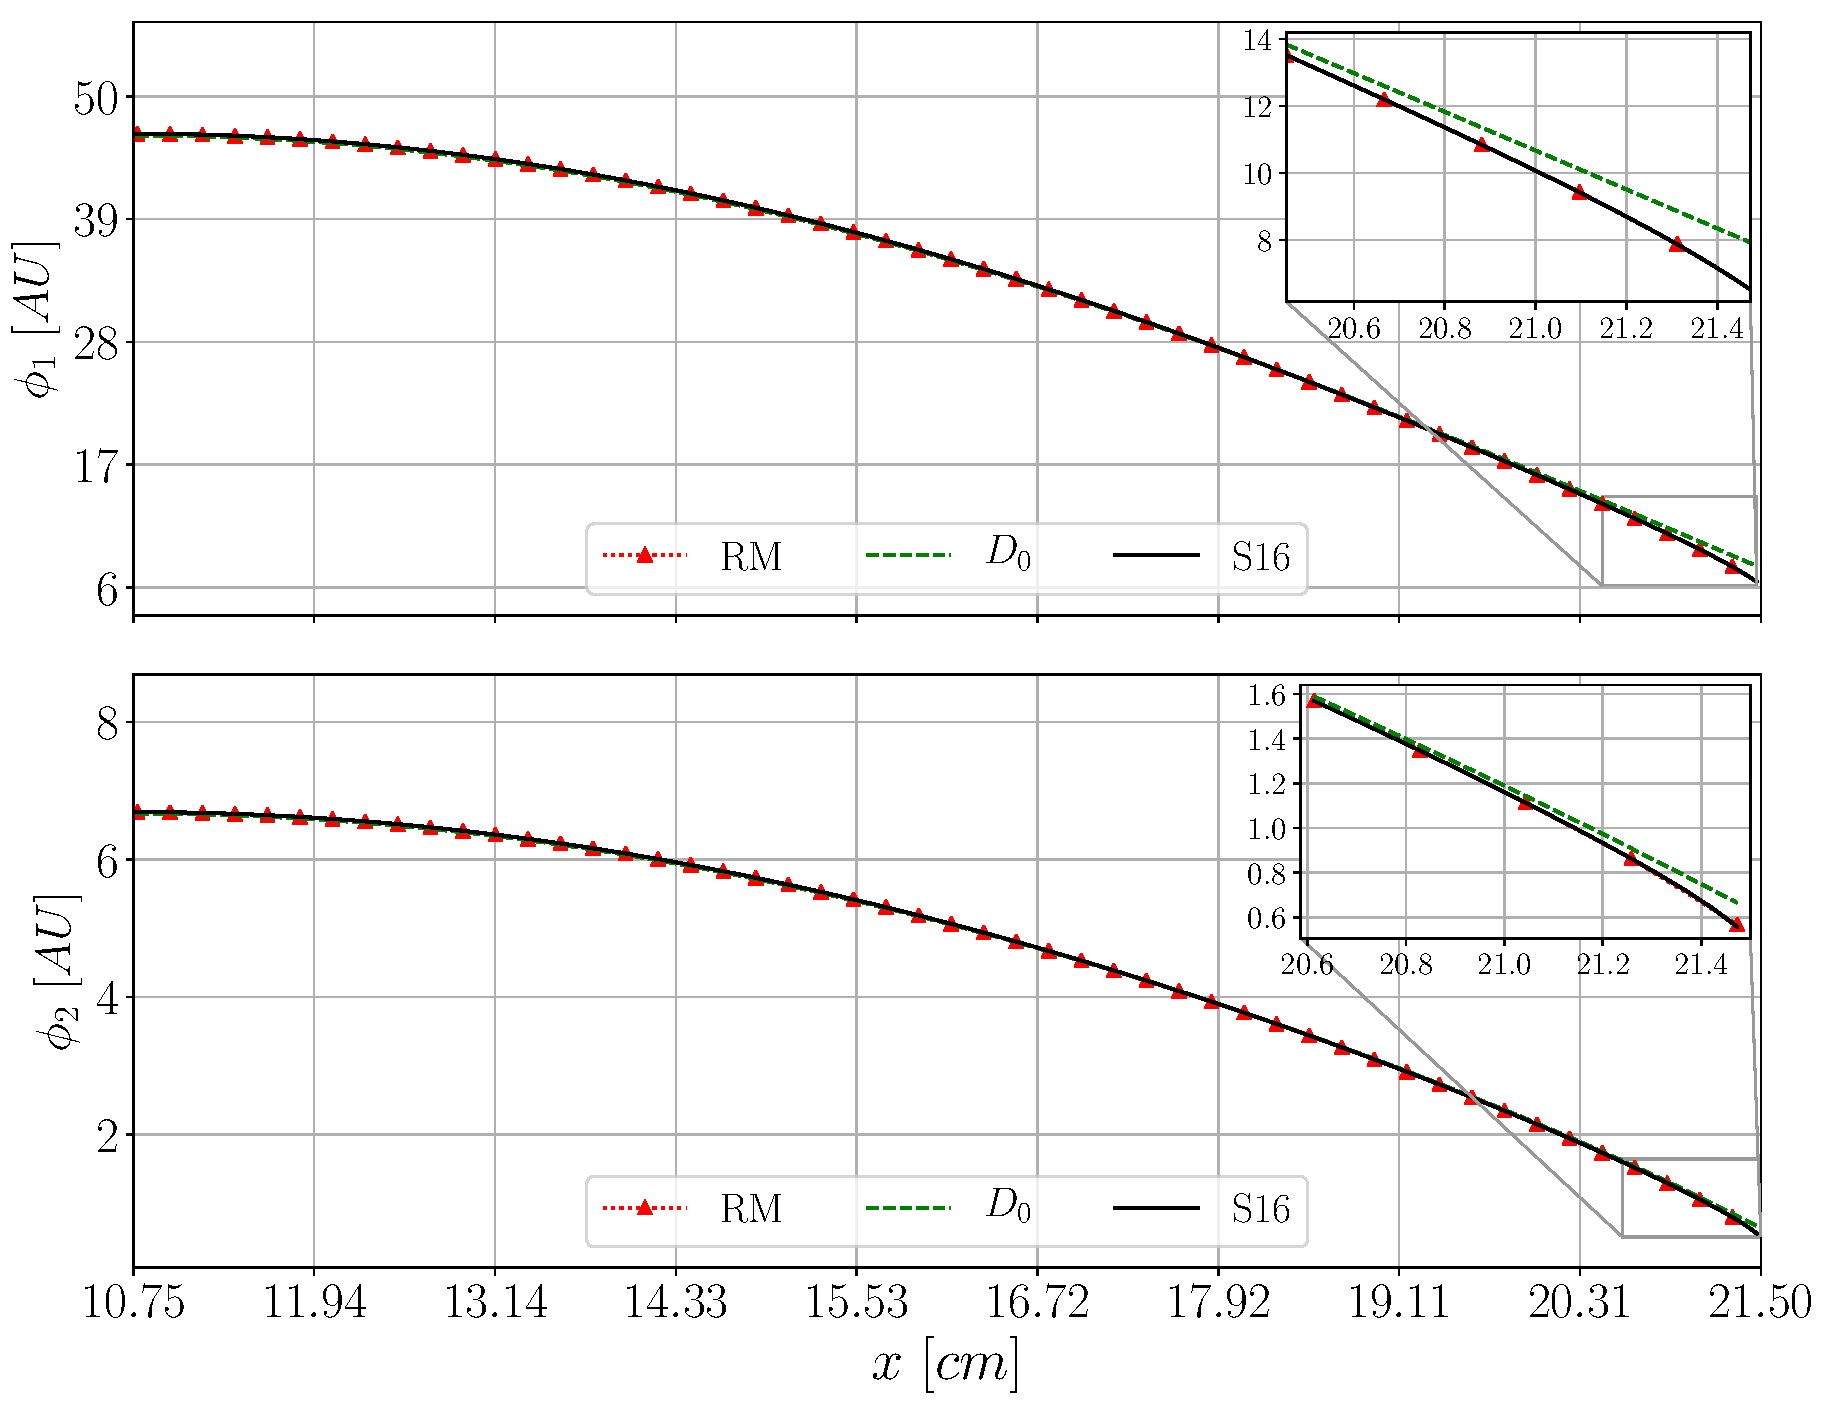
\includegraphics[width=0.7\linewidth]{Sn_Diff_Rm_flux_Tomatis2011.pdf}
	\caption{\DIFaddFL{Comparison of the fluxes as calculated by the reference S$_N$ code, the RM code, and a standard multigroup diffusion without RM correction ($D_0$). The insets show a zoom-in of the fluxes near the boundary. Results shown here after 250 Ronen iterations.}}
	\label{fig:slab-fluxes}		
\end{figure}

\begin{figure}[htbp]
	\centering
	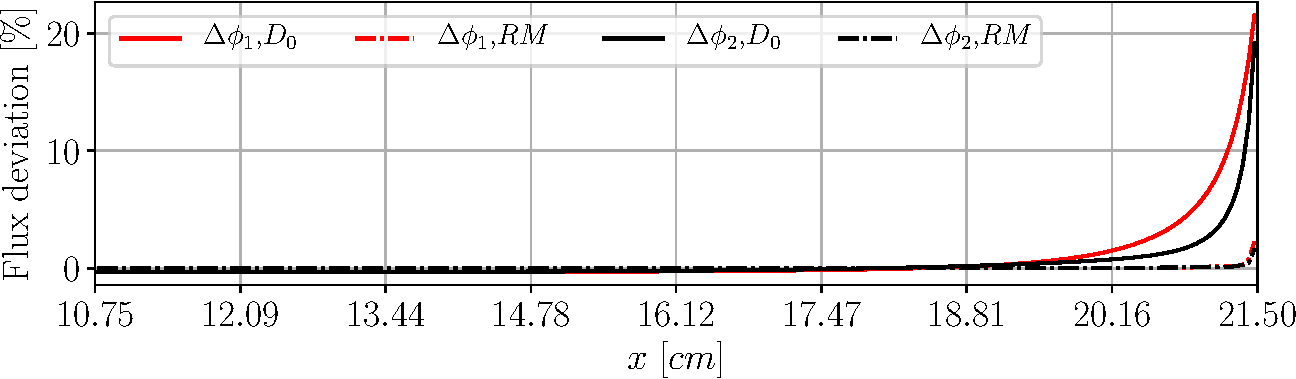
\includegraphics[width=0.65\linewidth]{flx_err_Tomatis2011_400_250.pdf}
	\caption{\DIFaddFL{Deviation of the fluxes with respect to the reference solution after 250 Ronen iterations.}}
	\label{fig:slab-fluxes-dev}
\end{figure}

\begin{figure}[htbp]
	\centering
	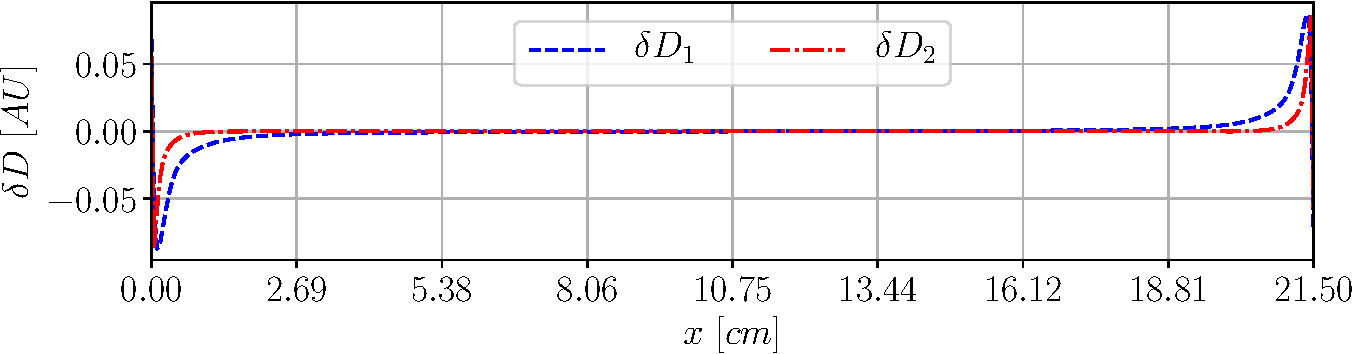
\includegraphics[width=0.65\linewidth]{dD_Tomatis2011_400_250it.pdf}
	\caption{\DIFaddFL{The Ronen method correction factors ($\delta D$). Results shown here after 250 Ronen iterations.}}
	\label{fig:slab-RM-corr-factor}
\end{figure}


%DIF > \begin{wrapfigure}{r}[0pt]{0.3\textwidth}
%DIF > 	\centering
%DIF > 	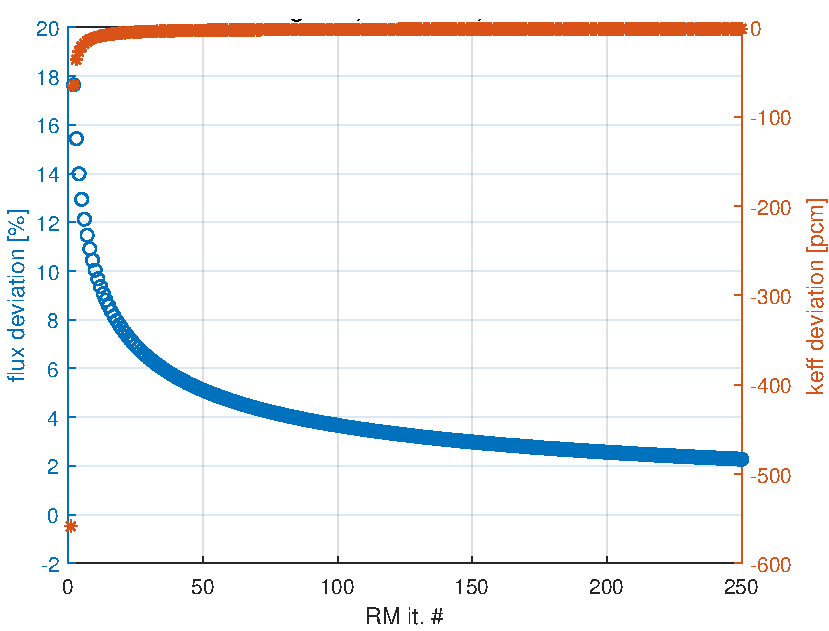
\includegraphics[width=\linewidth]{convergence.pdf}
%DIF > 	\caption{Convergence of the flux (max deviation) and the criticality eigenvalue.}
%DIF > 	\label{fig:conv}
%DIF > \end{wrapfigure} 

\begin{figure}[htbp]
	%DIF >  convergence
	\centering
	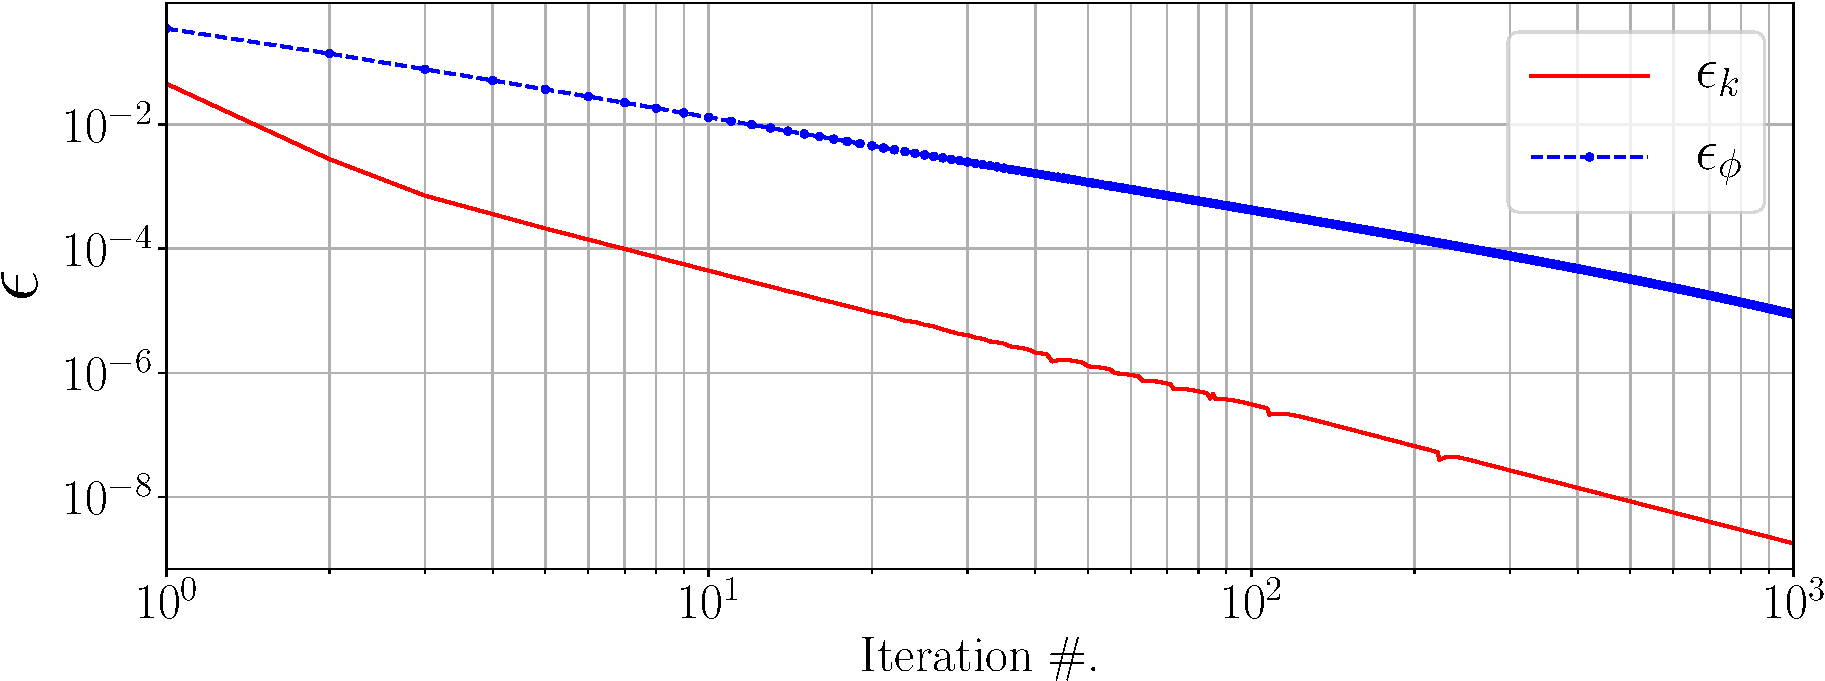
\includegraphics[width=0.65\linewidth]{epsilon1000.pdf}	
	%DIF > 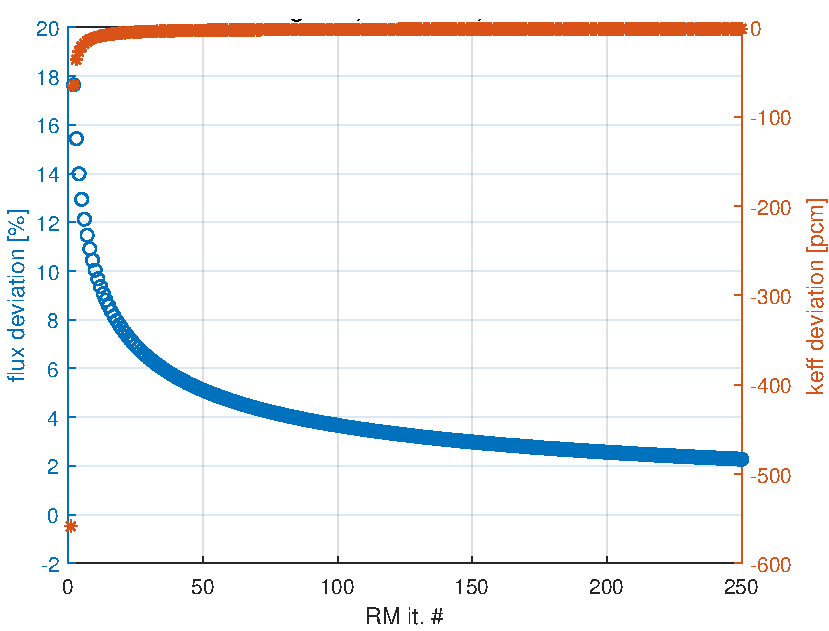
\includegraphics[width=0.4\linewidth]{convergence.pdf}
	\caption{\DIFaddFL{Convergence of the flux (max deviation) and of the criticality eigenvalue during 1000 Ronen iterations.}}
	\label{fig:conv}
\end{figure}

\DIFadd{The }\DIFaddend RM correction terms ($\delta D$) \DIFdelbegin \DIFdel{, and the corrected (spatially-dependent) diffusion $D$.It is clear }\DIFdelend \DIFaddbegin \DIFadd{along the slab are shown in Fig.~\ref{fig:slab-RM-corr-factor}. It is possible to observe }\DIFaddend that the diffusion correction \DIFdelbegin \DIFdel{assumes zero values }\DIFdelend \DIFaddbegin \DIFadd{almost vanishes }\DIFaddend at the slab center and \DIFdelbegin \DIFdel{exhibit }\DIFdelend \DIFaddbegin \DIFadd{exhibits }\DIFaddend non-trivial behavior near the boundary. The convergence of the flux (max deviation) and \DIFaddbegin \DIFadd{of }\DIFaddend the criticality eigenvalue are shown in Fig.~\ref{fig:conv}\DIFaddbegin \DIFadd{, where $\epsilon_\phi = \operatorname{max} [\phi^{(k)}-\phi^{(k-1)})/\phi^{(k-1)}]$ and $\epsilon_k = (k_\textrm{eff}^{(k)}-k_\textrm{eff}^{(k-1)})/k_\textrm{eff}^{(k-1)}$}\DIFaddend . While the eigenvalue converges within a few iterations, \DIFdelbegin \DIFdel{the flux exhibit slow convergence }\DIFdelend \DIFaddbegin \DIFadd{relatively slow convergence is noticed for the flux with higher differences against the reference S$_{16}$ solution }\DIFaddend near the boundaries. The spatial flux convergence between two successive Ronen iterations is shown in Fig.~\ref{fig:conv2} for the left half slab, according to \DIFdelbegin \DIFdel{$\Delta\phi = (\phi^{k-1}-\phi^k)/\phi^{k-1}$ }\DIFdelend \DIFaddbegin \DIFadd{$\Delta \phi = (\phi^{k-1}-\phi^k)/\phi^{k-1}$ }\DIFaddend [\%]. The spatial flux convergence of the Ronen iterations with respect to the reference \DIFdelbegin \DIFdel{$S_n$ }\DIFdelend solution for the left half slab is shown in Fig.~\ref{fig:conv3} \DIFaddbegin \DIFadd{instead}\DIFaddend .

%DIF <  fluxes
\DIFdelbegin %DIFDELCMD < \begin{figure}[htbp!]
%DIFDELCMD < 	%%%
\DIFdelendFL %DIF >  convergence
\DIFaddbeginFL \begin{figure}[htbp]
	\DIFaddendFL \centering
	\DIFdelbeginFL %DIFDELCMD < 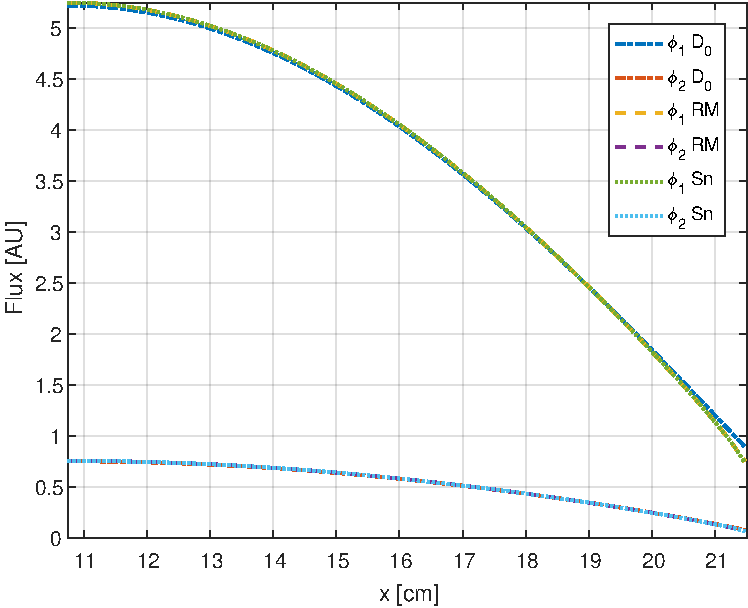
\includegraphics[width=0.45\linewidth]{flux0_half.pdf}
%DIFDELCMD < 	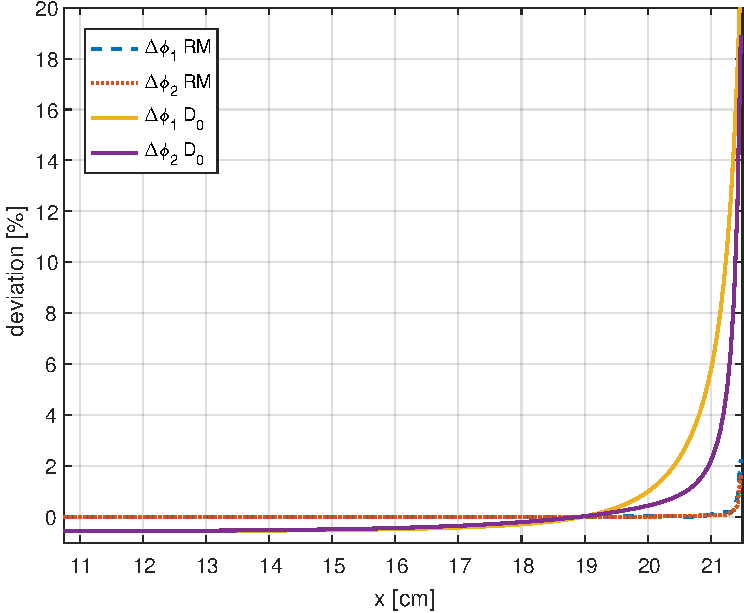
\includegraphics[width=0.45\linewidth]{flux_deviation_half.pdf}	
%DIFDELCMD < 	%%%
\DIFdelendFL \DIFaddbeginFL 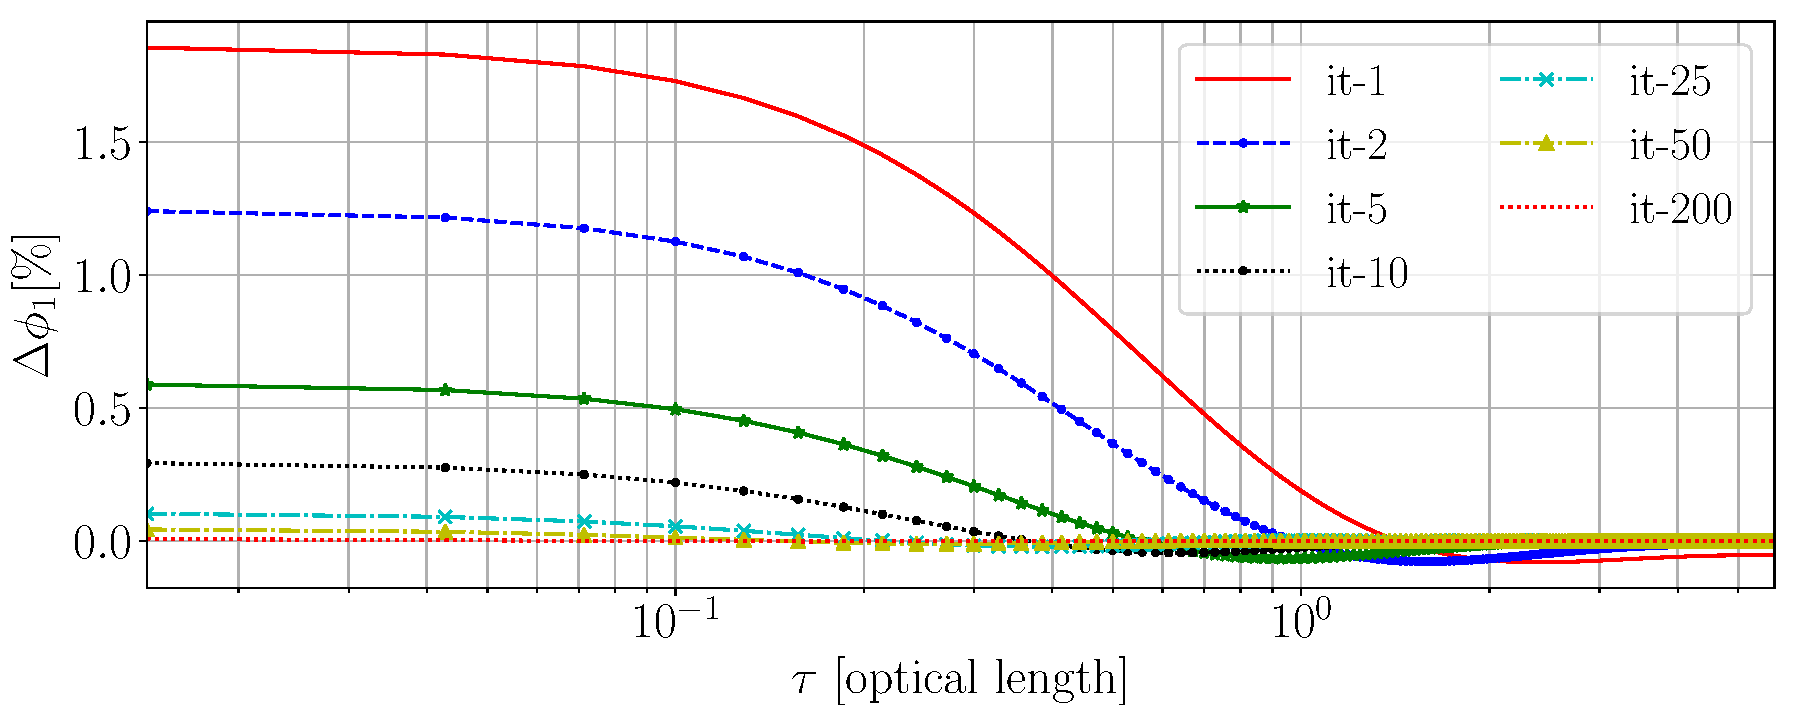
\includegraphics[width=0.65\linewidth]{fast_flx_err_RM.pdf}
	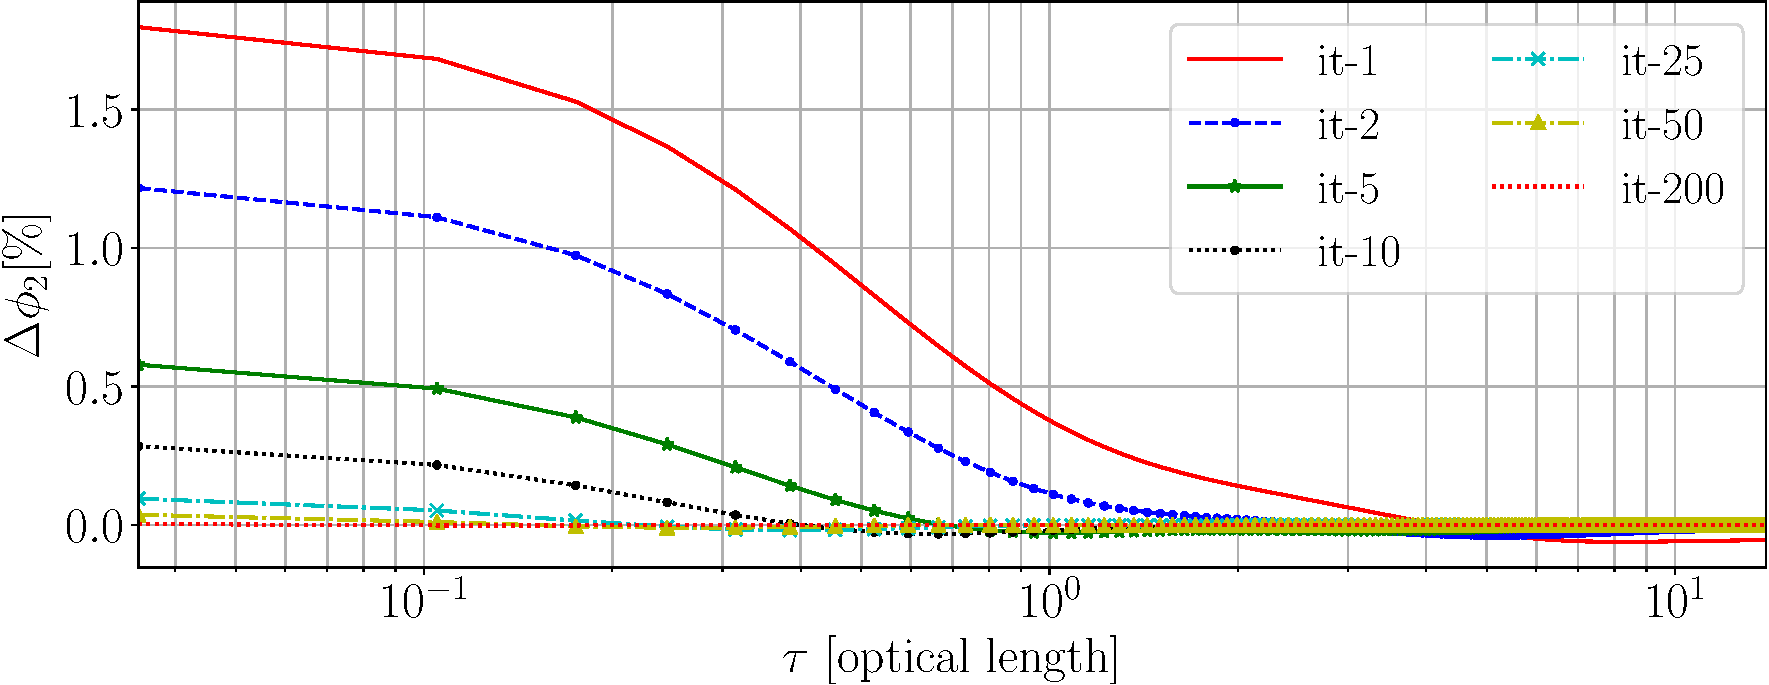
\includegraphics[width=0.65\linewidth]{thermal_flx_err_RM.pdf}	%DIF > 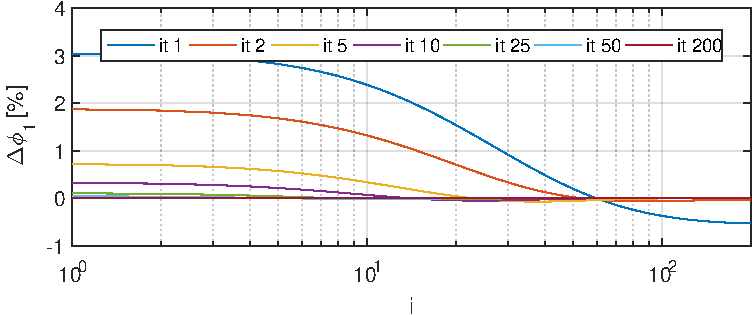
\includegraphics[width=0.48\linewidth]{flux_deviation_half_it_1.pdf}
	%DIF > 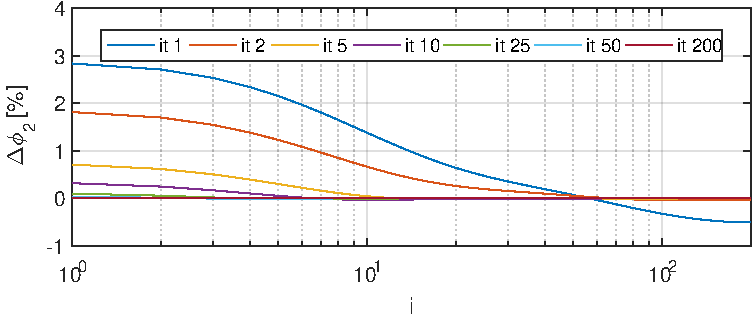
\includegraphics[width=0.48\linewidth]{flux_deviation_half_it_2.pdf}
	\DIFaddendFL \caption{\DIFdelbeginFL \DIFdelFL{Comparison of }\DIFdelendFL \DIFaddbeginFL \DIFaddFL{The spatial flux convergence between two successive Ronen iterations for }\DIFaddendFL the \DIFdelbeginFL \DIFdelFL{fluxes as calculated by the reference $S_n$ code}\DIFdelendFL \DIFaddbeginFL \DIFaddFL{left half slab}\DIFaddendFL , \DIFdelbeginFL \DIFdelFL{the RM code, and a standard multigroup diffusion w/o RM correction ($D_0$)}\DIFdelendFL \DIFaddbeginFL \DIFaddFL{according to $\Delta\phi = (\phi^{(k-1)}-\phi^{(k)})/\phi^{(k-1)}$ }[\DIFaddFL{\%}]\DIFaddendFL .\DIFdelbeginFL \DIFdelFL{Results shown here after 250 Ronen iterations.}\DIFdelendFL }
	\DIFdelbeginFL %DIFDELCMD < \label{fig:fluxes}
%DIFDELCMD < %%%
\DIFdelendFL \DIFaddbeginFL \label{fig:conv2}
\DIFaddendFL \end{figure}

%DIF <  current
\DIFdelbegin %DIFDELCMD < \begin{figure}[htbp!]
%DIFDELCMD < 	%%%
\DIFdelendFL %DIF >  convergence
\DIFaddbeginFL \begin{figure}[hbtp]
	\DIFaddendFL \centering
	%DIF < 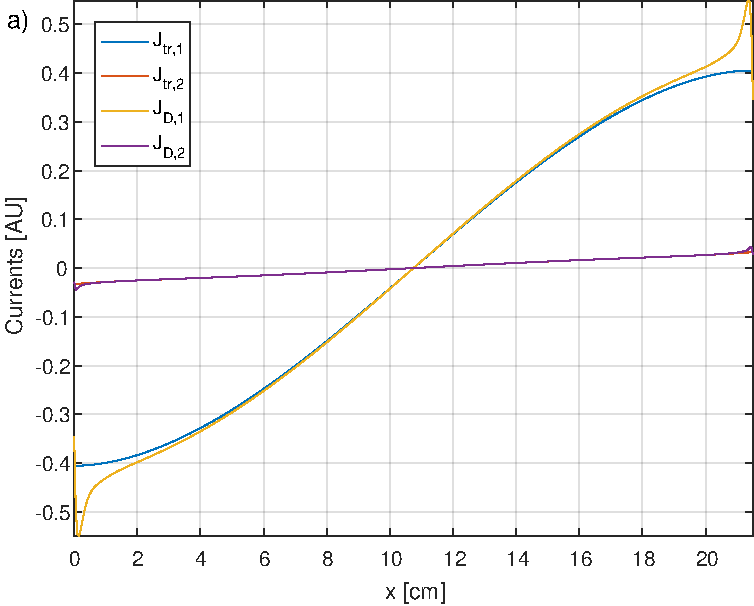
\includegraphics[width=0.45\linewidth]{current.pdf}
	\DIFdelbeginFL %DIFDELCMD < 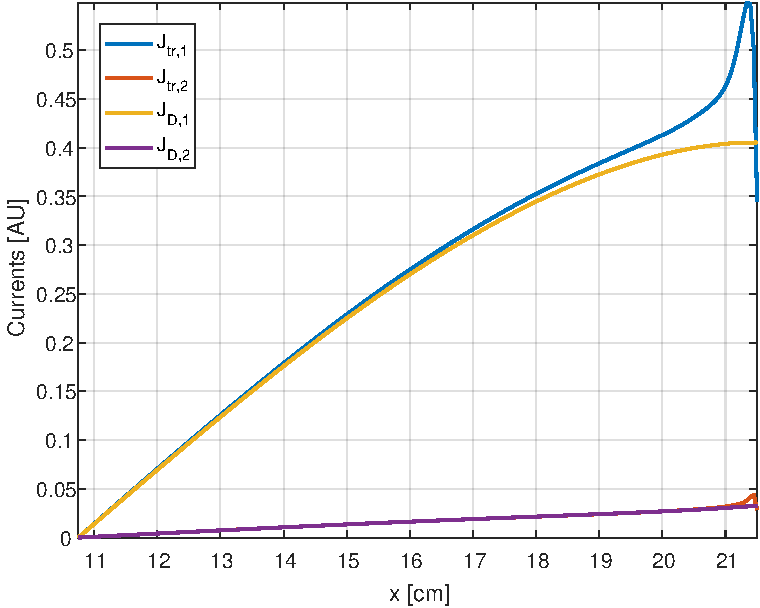
\includegraphics[width=0.45\linewidth]{current_half.pdf}	
%DIFDELCMD < 	%%%
\DIFdelendFL \DIFaddbeginFL 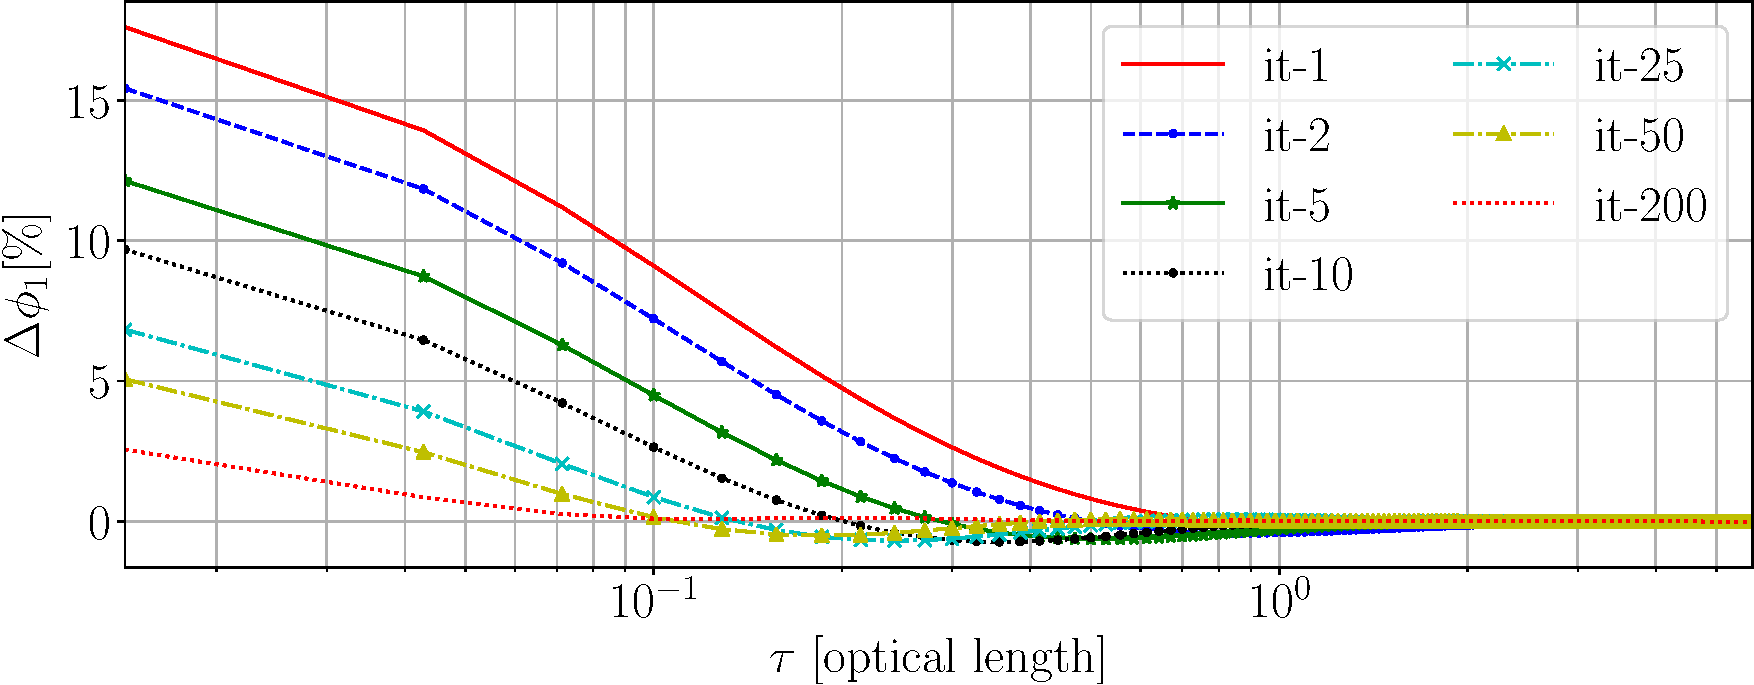
\includegraphics[width=0.65\linewidth]{RM_Sn_converg_FAST.pdf}
	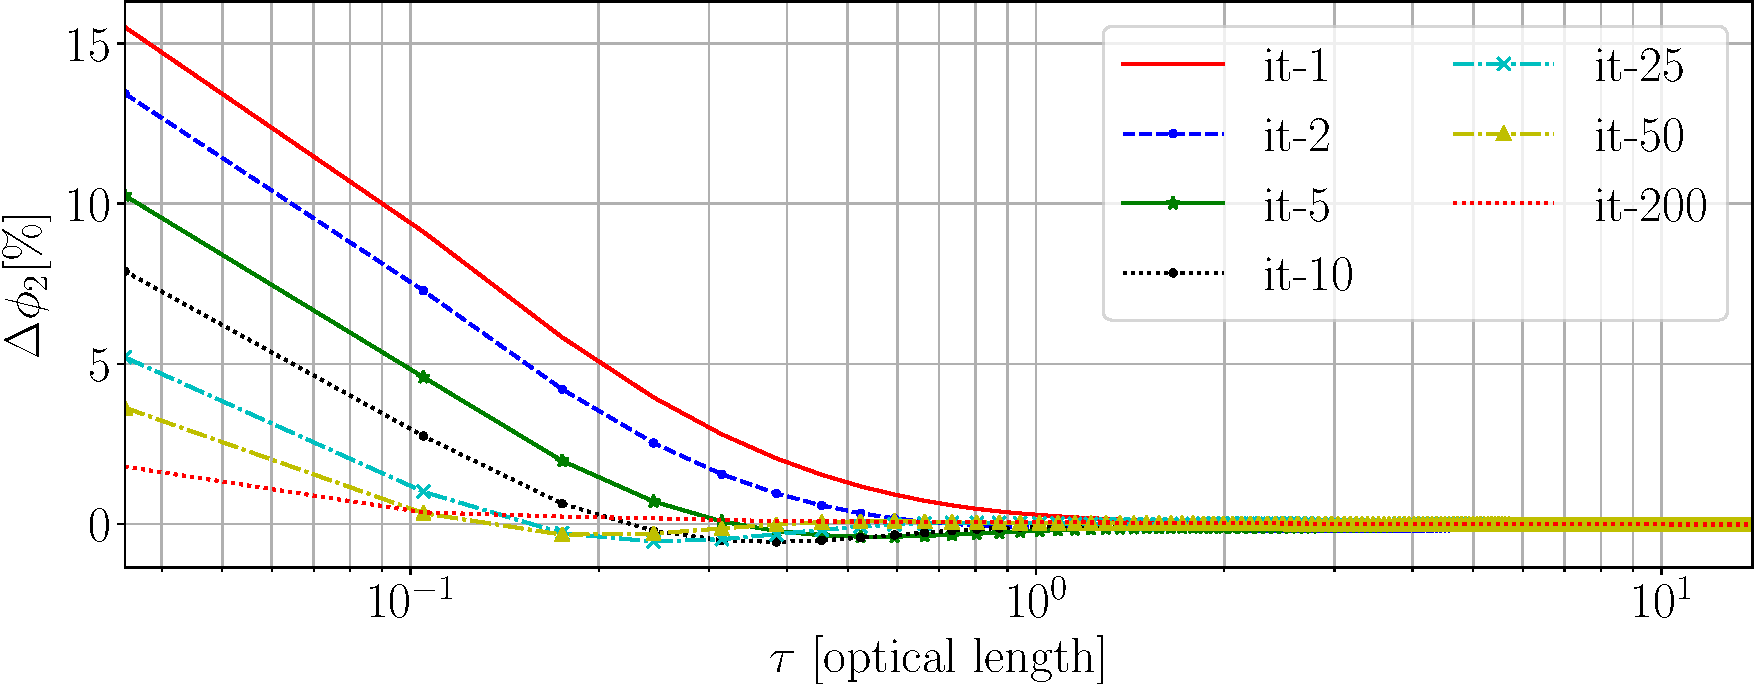
\includegraphics[width=0.65\linewidth]{RM_Sn_converg_THERMAL.pdf}
	\DIFaddendFL \caption{The \DIFdelbeginFL \DIFdelFL{diffusion and transport currents calculated using }\DIFdelendFL \DIFaddbeginFL \DIFaddFL{spatial flux convergence of }\DIFaddendFL the \DIFdelbeginFL \DIFdelFL{converged }\DIFdelendFL Ronen \DIFaddbeginFL \DIFaddFL{iterations with respect to the reference S$_{16}$ }\DIFaddendFL solution \DIFaddbeginFL \DIFaddFL{for the left half slab}\DIFaddendFL .}
	\DIFdelbeginFL %DIFDELCMD < \label{fig:current}
%DIFDELCMD < %%%
\DIFdelendFL \DIFaddbeginFL \label{fig:conv3}
\DIFaddendFL \end{figure}

%DIF <  D-coef
\DIFdelbegin %DIFDELCMD < \begin{figure}[htbp!]
%DIFDELCMD < 	%%%
\DIFdelendFL \DIFaddbeginFL \DIFaddFL{Notice the change of sign in the flux convergence $\Delta \phi$ in Fig.~\ref{fig:conv2} between the center (negative) and the boundary (positive) of the slab. The initial diffusion solution is smoother than the transport one. Hence, it can be seen in Fig.~\ref{fig:slab-fluxes} that the diffusion solution underestimates the peak flux at the center of the slab and overestimates the flux near the boundary. The Ronen iterations ``push'' the diffusion solution towards the transport one by increasing the flux level at the center of the slab and decreasing the flux level at the boundary. Hence, $\phi^{(k-1)}$ is smaller at the center and higher at the boundary compared to $\phi^{(k)}$. This effect caused by Ronen iterations produces less smooth flux shape with steeper gradients comparing to the diffusion solution.
%DIF > 
%DIF >  ---------------------------------------------------
}\subsection{\DIFaddFL{Heterogeneous case}}
\label{subsec:heterog}

\DIFaddFL{The heterogeneous benchmark defines three heterogeneous cores, each is 7 fuel assemblies long and comprised of four different fuel assemblies made of four different materials~\mbox{%DIFAUXCMD
\cite{Rahnema-1997}}\hspace{0pt}%DIFAUXCMD
, as shown in Fig.~\ref{fig:hetro-core}. Material properties for each region of the assemblies are given in Table~\ref{tab:xs2}. Configuration 1 represents the least heterogeneous core with rather smooth flux gradients. On the contrary, configuration 3 represents the most heterogeneous core with the steepest flux gradients and can serve as a limiting case~\mbox{%DIFAUXCMD
\cite{Rahnema-1997}}\hspace{0pt}%DIFAUXCMD
. Void boundary conditions are imposed on both ends of the core. 
}

\begin{figure}[htbp] 
	\DIFaddendFL \centering
	\DIFdelbeginFL %DIFDELCMD < 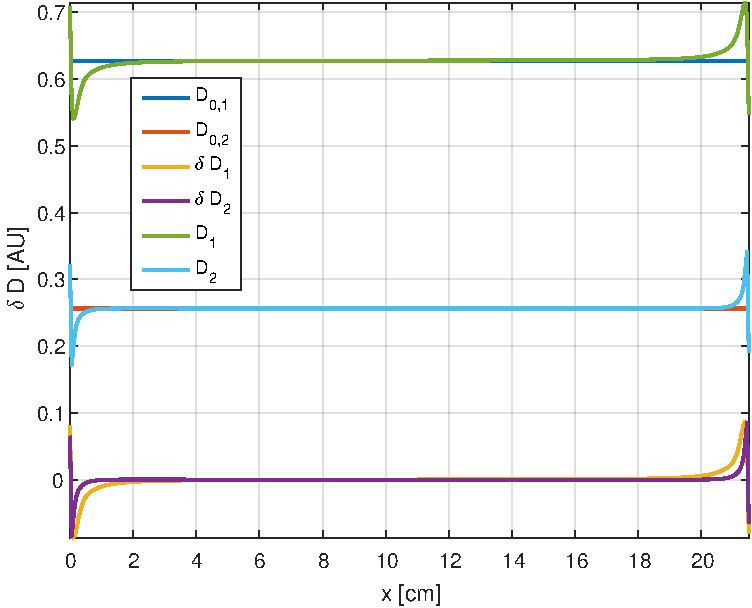
\includegraphics[width=0.45\linewidth]{D_coeffs.pdf}
%DIFDELCMD < 	%%%
%DIF < 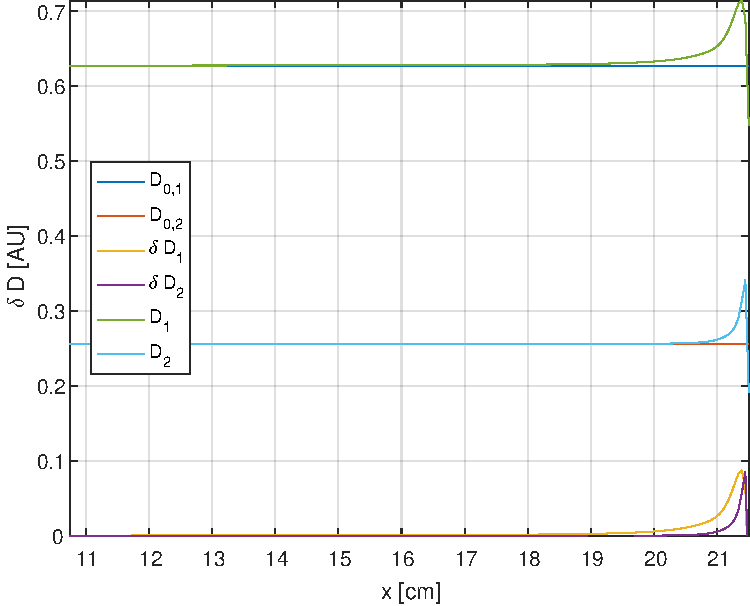
\includegraphics[width=0.45\linewidth]{D_coeffs_half.pdf}	
	\DIFdelendFL \DIFaddbeginFL \begin{tikzpicture}
	% -------------- Assembly 1 --------------
	\node[above] at (-2,1.5) {Assembly A1};
	\draw[pattern=north west lines, preaction={fill=blue!70}] (-3,0)   rectangle (-2.8,1.5);
	\draw[pattern=dots, preaction={fill=yellow!50}] 		  (-2.8,0) rectangle (-2.4,1.5);
	\draw[fill=red!80] 										  (-2.4,0) rectangle (-2,1.5);
	\draw[fill=red!80]	  									  (-2,0)   rectangle (-1.6,1.5);
	\draw[pattern=dots, preaction={fill=yellow!50}] 		  (-1.6,0) rectangle (-1.2,1.5);
	\draw[pattern=north west lines, preaction={fill=blue!70}] (-1.2,0) rectangle (-1,1.5);
	% -------------- Assembly 2 --------------
	\node[above] at (1,1.5) {Assembly A2};
	\draw[pattern=north west lines, preaction={fill=blue!70}] (0,0)	  rectangle (0.2,1.5);
	\draw[pattern=dots, preaction={fill=yellow!50}] 		  (0.2,0) rectangle (0.6,1.5);
	\draw[pattern=dots, preaction={fill=yellow!50}] 		  (0.6,0) rectangle (1,1.5);
	\draw[pattern=dots, preaction={fill=yellow!50}] 		  (1,0)   rectangle (1.4,1.5);
	\draw[pattern=dots, preaction={fill=yellow!50}] 		  (1.4,0) rectangle (1.8,1.5);
	\draw[pattern=north west lines, preaction={fill=blue!70}] (1.8,0) rectangle (2,1.5);
	% -------------- Assembly 3 --------------
	\node[above] at (-2,-1) {Assembly A3};
	\draw[pattern=north west lines, preaction={fill=blue!70}]  (-3,-2.5)   rectangle (-2.8,-1);
	\draw[pattern=dots, preaction={fill=yellow!50}] 		   (-2.8,-2.5) rectangle (-2.4,-1);
	\draw[pattern=north east lines, preaction={fill=green!50}] (-2.4,-2.5) rectangle (-2,-1);
	\draw[pattern=north east lines, preaction={fill=green!50}] (-2,-2.5)   rectangle (-1.6,-1);
	\draw[pattern=dots, preaction={fill=yellow!50}] 		   (-1.6,-2.5) rectangle (-1.2,-1);
	\draw[pattern=north west lines, preaction={fill=blue!70}] (-1.2,-2.5)  rectangle (-1,-1);
	\draw [<->] (-3,-2.7) -- node[below]{15.24 [cm]}	(-1,-2.7);
	% -------------- Assembly 4 --------------
	\node[above] at (1,-1) {Assembly A4};
	\draw[pattern=north west lines, preaction={fill=blue!70}]  (0,-2.5)    rectangle (0.2,-1); 
	\draw[pattern=north east lines, preaction={fill=green!50}] (0.2,-2.5)  rectangle (0.6,-1);
	\draw[pattern=north east lines, preaction={fill=green!50}] (0.6,-2.5)  rectangle (1,-1);
	\draw[pattern=north east lines, preaction={fill=green!50}] (1,-2.5)    rectangle (1.4,-1);
	\draw[pattern=north east lines, preaction={fill=green!50}] (1.4,-2.5)  rectangle (1.8,-1);
	\draw[pattern=north west lines, preaction={fill=blue!70}]  (1.8,-2.5)  rectangle (2,-1);
	% -------------- Core 1 --------------
	\node[] at (3.2,1) {Core 1};
	\draw [fill=orange!80]   (4,0.5)   rectangle node{A1} 	(5,1.5);
	\draw [fill=gray!90] 	 (5,0.5)   rectangle node{A2}	(6,1.5);
	\draw [fill=orange!80]   (6,0.5)   rectangle node{A1}	(7,1.5);
	\draw [fill=gray!90] 	 (7,0.5)   rectangle node{A2}	(8,1.5);
	\draw [fill=orange!80]   (8,0.5)   rectangle node{A1}	(9,1.5);
	\draw [fill=gray!90] 	 (9,0.5)   rectangle node{A2}	(10,1.5);
	\draw [fill=orange!80]   (10,0.5)  rectangle node{A1}	(11,1.5);
	% -------------- Core 2 --------------
	\node[] at (3.2,-0.5) {Core 2};
	\draw [fill=orange!80]   (4,-1)   rectangle node{A1}	(5,-0);
	\draw [fill=gray!40] 	 (5,-1)   rectangle node{A3}	(6,-0);
	\draw [fill=orange!80]   (6,-1)   rectangle node{A1}	(7,-0);
	\draw [fill=gray!40] 	 (7,-1)   rectangle node{A3}	(8,-0);
	\draw [fill=orange!80]   (8,-1)   rectangle node{A1}	(9,-0);
	\draw [fill=gray!40] 	 (9,-1)   rectangle node{A3}	(10,-0);
	\draw [fill=orange!80]   (10,-1)  rectangle node{A1}	(11,-0);
	% -------------- Core 3 --------------
	\node[] at (3.2,-2) {Core 3};
	\draw [fill=orange!80]  (4,-2.5)  rectangle node{A1} 	(5,-1.5);
	\draw [fill=white] 		(5,-2.5)  rectangle node{A4}	(6,-1.5);
	\draw [fill=orange!80]  (6,-2.5)  rectangle node{A1}	(7,-1.5);
	\draw [fill=white] 		(7,-2.5)  rectangle node{A4}	(8,-1.5);
	\draw [fill=orange!80]  (8,-2.5)  rectangle node{A1}	(9,-1.5);
	\draw [fill=white] 		(9,-2.5)  rectangle node{A4}	(10,-1.5);
	\draw [fill=orange!80]  (10,-2.5) rectangle node{A1}	(11,-1.5);
	\draw [<->] (4,-2.8) -- node[below]{106.68 [cm]}	(11,-2.8);
	\end{tikzpicture}
	\DIFaddendFL \caption{\DIFdelbeginFL \DIFdelFL{The original standard diffusion coefficients ($D=(3\sigma_{tr})^{-1}$),
		}\DIFdelendFL \DIFaddbeginFL \DIFaddFL{Schematic illustration of }\DIFaddendFL the \DIFdelbeginFL \DIFdelFL{RM correction terms ($\delta D$), }\DIFdelendFL \DIFaddbeginFL \DIFaddFL{fuel assemblies }\DIFaddendFL and \DIFdelbeginFL \DIFdelFL{the corrected (spatially-dependent)
		diffusion $D$}\DIFdelendFL \DIFaddbeginFL \DIFaddFL{core composition and geometry~\mbox{%DIFAUXCMD
\cite{Rahnema-1997}}\hspace{0pt}%DIFAUXCMD
}\DIFaddendFL .\DIFdelbeginFL \DIFdelFL{Results shown here after 250 Ronen iterations.}\DIFdelendFL }
	\DIFdelbeginFL %DIFDELCMD < \label{fig:Dcoef}
%DIFDELCMD < %%%
\DIFdelendFL \DIFaddbeginFL \label{fig:hetro-core}	
\DIFaddendFL \end{figure}


%DIF <  convergence
\DIFaddbegin \begin{table}[htbp]	
	\centering
	\caption{\DIFaddFL{Two-group macroscopic cross sections }[\DIFaddFL{cm\tsup{-1}}] \DIFaddFL{used for the heterogeneous case~\mbox{%DIFAUXCMD
\cite{Rahnema-1997}}\hspace{0pt}%DIFAUXCMD
. Colors are in accordance with Fig.~\ref{fig:hetro-core}.}} 
	\label{tab:xs2}
	\begin{tabular}{lcccccccr}
		\DIFaddFL{Material}&\DIFaddFL{$\sigma_1$}&\DIFaddFL{$\sigma_2$}&\DIFaddFL{$\nu\sigma_{f,1}$}&\DIFaddFL{$\nu\sigma_{f,2}$}&\DIFaddFL{$\sigma_{s,1\leftarrow 1}$}&\DIFaddFL{$\sigma_{s,2\leftarrow 1}$}&\DIFaddFL{$\sigma_{s,2\leftarrow 2}$}&\DIFaddFL{$x$ }[\DIFaddFL{cm}]\\
		\midrule
		\DIFaddFL{Water  (Blue)	}&\DIFaddFL{0.1890	 }&\DIFaddFL{1.4633  }&\DIFaddFL{0.0000	 }&\DIFaddFL{0.0000	 }&\DIFaddFL{0.1507   }&\DIFaddFL{0.0380		}&\DIFaddFL{1.4536		 }&\DIFaddFL{1.158}\\
		\DIFaddFL{Fuel 1 (Red)	}&\DIFaddFL{0.2263  }&\DIFaddFL{1.0119  }&\DIFaddFL{0.0067	 }&\DIFaddFL{0.1241	 }&\DIFaddFL{0.2006   }&\DIFaddFL{0.0161		}&\DIFaddFL{0.9355		 }&\DIFaddFL{3.231}\\
		\DIFaddFL{Fuel 2 (Yellow)	}&\DIFaddFL{0.2252  }&\DIFaddFL{0.9915  }&\DIFaddFL{0.0078	 }&\DIFaddFL{0.1542 	 }&\DIFaddFL{0.1995   }&\DIFaddFL{0.0156		}&\DIFaddFL{0.9014		 }&\DIFaddFL{3.231}\\
		\DIFaddFL{Fuel 3 (Green)	}&\DIFaddFL{0.2173  }&\DIFaddFL{1.0606  }&\DIFaddFL{0.0056	 }&\DIFaddFL{0.0187	 }&\DIFaddFL{0.1902   }&\DIFaddFL{0.0136		}&\DIFaddFL{0.5733 	 }&\DIFaddFL{3.231}\\
	\end{tabular}
\end{table}

%DIF > \newpage
\DIFadd{Table~\ref{tab:dx_drho2} shows the reactivity differences between standard diffusion (with extrapolated length) and the Ronen method (at increasing number of iterations) with respect to the reference solution for each of the three core configurations. The standard diffusion solution perform rather well for core 1 with deviation of 182 pcm, but fails for cores 2 and 3 with deviation of 773 and 3335 pcm, respectively. This is explained by the fact that cores 2 and 3 are more heterogeneous compared to core 1. The Ronen method performs better than standard diffusion for all three cores, even after merely 10 iterations. Additional Ronen iterations further improve the estimated multiplication factor until convergence within the prescribed tolerance.      
}

\begin{table}[htbp]
	\centering
	\caption{\DIFaddFL{Reactivity differences as a function of number of iterations using the Ronen method. 728 nodes.}}
	\label{tab:dx_drho2}
	\begin{tabular}{lcccccr}
		%DIF > \midrule
		\DIFaddFL{Method }& \multicolumn{2}{c}{Core 1} & \multicolumn{2}{c}{Core 2} & \multicolumn{2}{c}{Core 3}  \\ 
		\midrule
		{}				& \DIFaddFL{$\keff$}& \DIFaddFL{$\Delta\rho$ }[\DIFaddFL{pcm}]& \DIFaddFL{$\keff$	}&\DIFaddFL{$\Delta\rho$ }[\DIFaddFL{pcm}]& \DIFaddFL{$\keff$ }&\DIFaddFL{$\Delta\rho$ }[\DIFaddFL{pcm}] \\
		\DIFaddFL{S$_{16}$		}&\DIFaddFL{1.25614	}&\DIFaddFL{-			 }&\DIFaddFL{1.00094   }&\DIFaddFL{-				  }&\DIFaddFL{0.79878		}&\DIFaddFL{-		}\\
		\DIFaddFL{Diffusion		}&\DIFaddFL{1.25902	}&\DIFaddFL{182		 }&\DIFaddFL{0.99325	}&\DIFaddFL{-773			  }&\DIFaddFL{0.77805		}&\DIFaddFL{-3335	}\\
		\DIFaddFL{RM-10			}&\DIFaddFL{1.25677	}&\DIFaddFL{40			 }&\DIFaddFL{1.00107	}&\DIFaddFL{13			 	  }&\DIFaddFL{0.79824		}&\DIFaddFL{-85	}\\
		\DIFaddFL{RM-20			}&\DIFaddFL{1.25648	}&\DIFaddFL{22			 }&\DIFaddFL{1.00091	}&\DIFaddFL{-3			  	  }&\DIFaddFL{0.79837		}&\DIFaddFL{-64	}\\
		\DIFaddFL{RM-50			}&\DIFaddFL{1.25625	}&\DIFaddFL{7			 }&\DIFaddFL{1.00076	}&\DIFaddFL{-18			  }&\DIFaddFL{0.79839		}&\DIFaddFL{-61	}\\
		\DIFaddFL{RM-100			}&\DIFaddFL{1.25618	}&\DIFaddFL{3			 }&\DIFaddFL{1.00070	}&\DIFaddFL{-24			  }&\DIFaddFL{0.79838		}&\DIFaddFL{-62	}\\		
	\end{tabular}
\end{table}

\DIFadd{The two-group flux distribution across each core is shown in Fig.~\ref{fig:hetero-flux} for standard diffusion ($D_0$), Ronen method (RM) and the S$_{16}$ reference solution. RM results are shown for 100 iterations and the spatial mesh spans 8 nodes in the water and 22 nodes in each fuel element. On a first glance, it is easy to see that standard diffusion fails to produce the steep flux gradients across material interfaces, especially between fuel and water. This is more pronounced for the fast flux, where even in core 1 it is not described correctly. 
%DIF > 
}\DIFaddend \begin{figure}[htbp!]
	\centering
	\DIFdelbeginFL %DIFDELCMD < 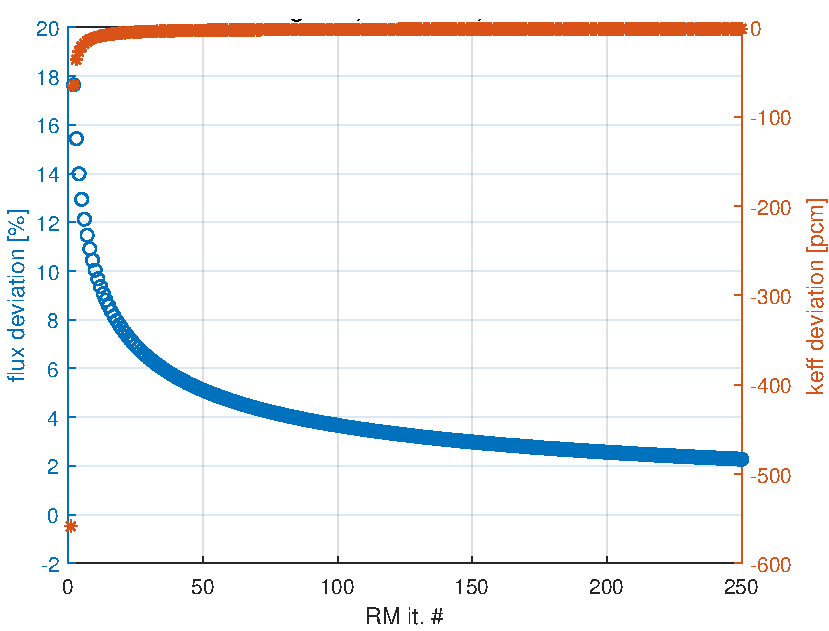
\includegraphics[width=0.45\linewidth]{convergence.pdf}
%DIFDELCMD < 	%%%
\DIFdelendFL \DIFaddbeginFL 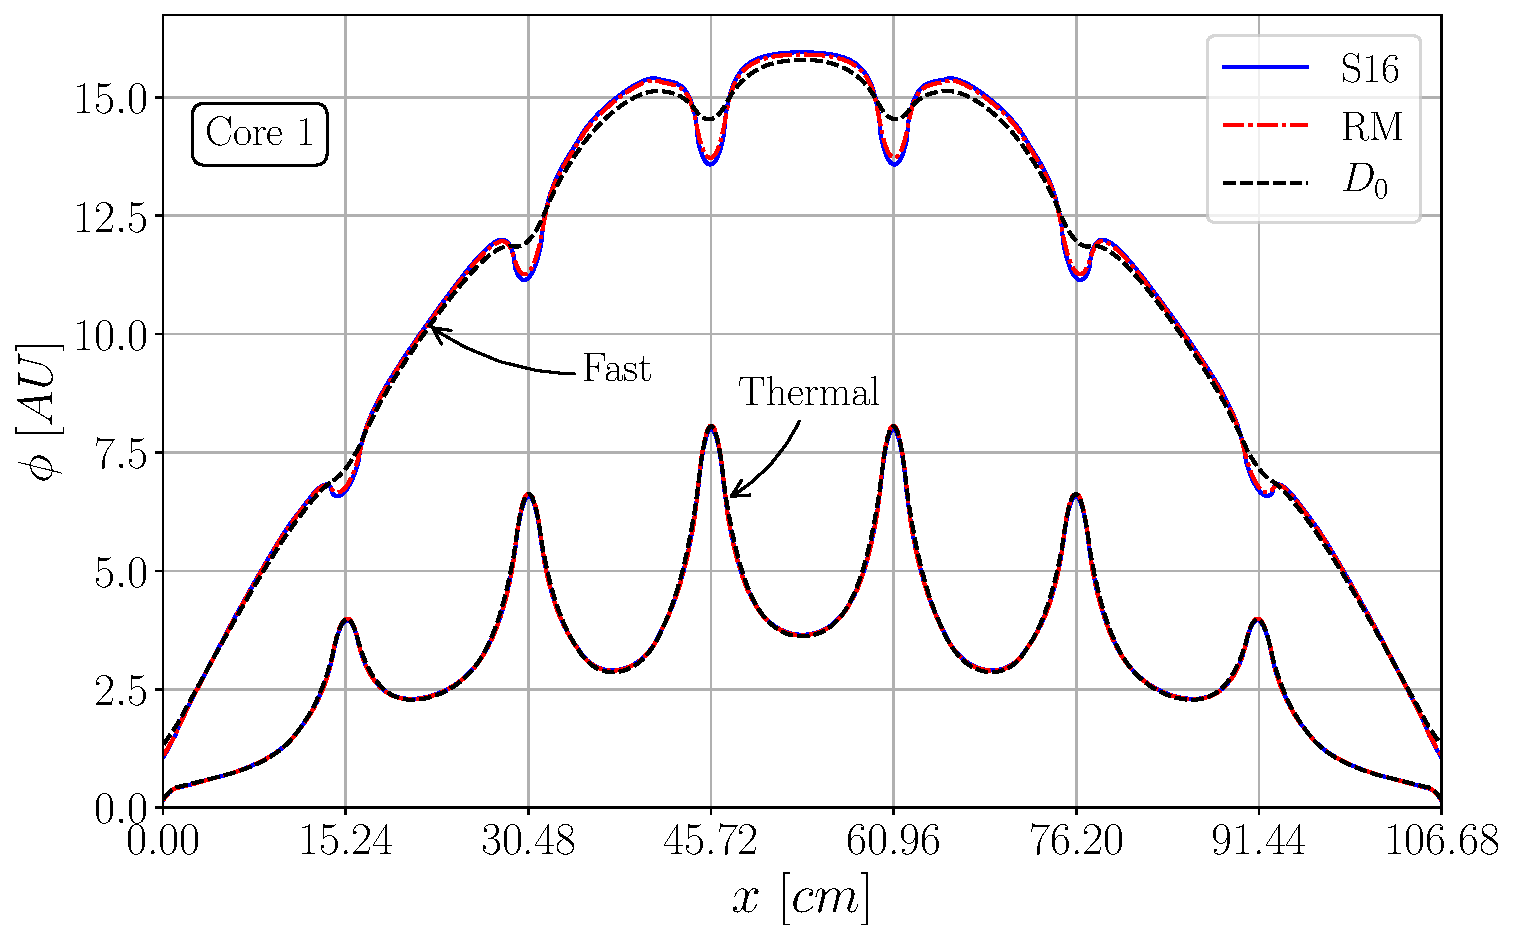
\includegraphics[width=0.49\linewidth]{Sn_Diff_RM_core_1.pdf}
	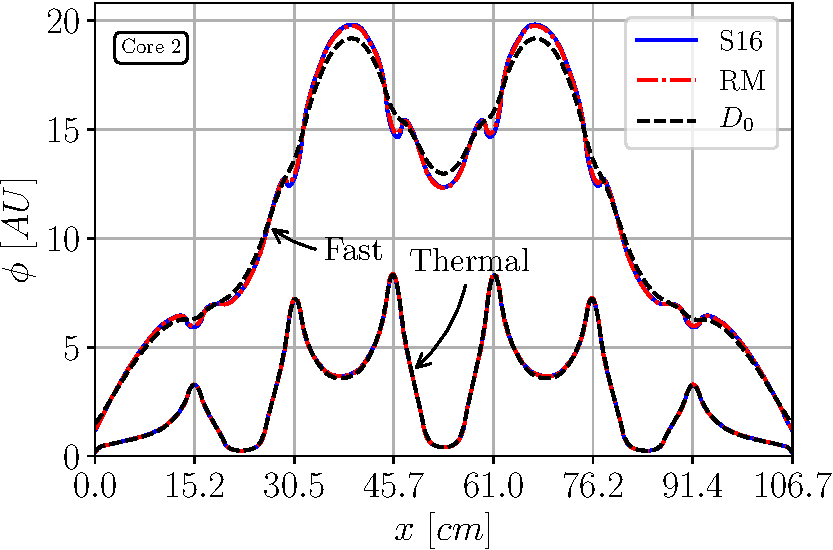
\includegraphics[width=0.49\linewidth]{Sn_Diff_RM_core_2.pdf}
	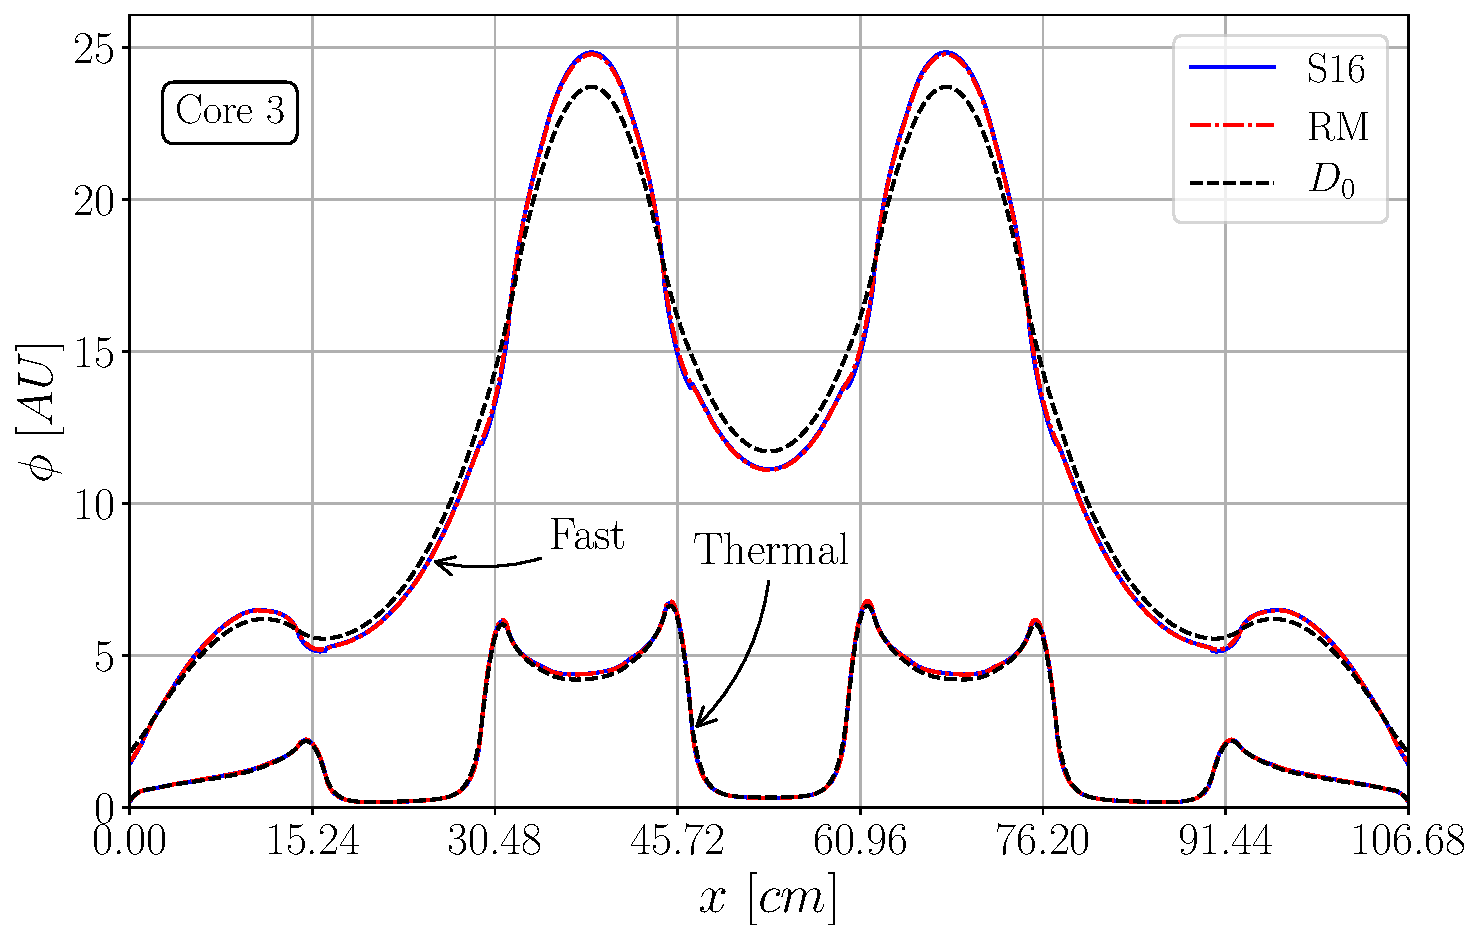
\includegraphics[width=0.49\linewidth]{Sn_Diff_RM_core_3.pdf}
	\DIFaddendFL \caption{\DIFdelbeginFL \DIFdelFL{Convergence of the }\DIFdelendFL \DIFaddbeginFL \DIFaddFL{Fast and thermal }\DIFaddendFL flux \DIFaddbeginFL \DIFaddFL{for each core using standard diffusion }\DIFaddendFL (\DIFdelbeginFL \DIFdelFL{max deviation}\DIFdelendFL \DIFaddbeginFL \DIFaddFL{$D_0$}\DIFaddendFL )\DIFaddbeginFL \DIFaddFL{, Ronen method (RM) }\DIFaddendFL and \DIFaddbeginFL \DIFaddFL{S$_{16}$ reference solution. Vertical grid lines are located at assemblies interfaces. RM results are for 100 iterations and }\DIFaddendFL the \DIFdelbeginFL \DIFdelFL{criticality
		eigenvalue}\DIFdelendFL \DIFaddbeginFL \DIFaddFL{spatial mesh spans 8 nodes in the water and 22 nodes in each fuel element}\DIFaddendFL .}
	\DIFdelbeginFL %DIFDELCMD < \label{fig:conv}
%DIFDELCMD < %%%
\DIFdelendFL \DIFaddbeginFL \label{fig:hetero-flux}
\DIFaddendFL \end{figure}

%DIF <  convergence
\DIFdelbegin %DIFDELCMD < \begin{figure}[htbp!]
%DIFDELCMD < 	%%%
\DIFdelendFL \DIFaddbeginFL \DIFaddFL{The fast and thermal flux deviation of standard diffusion ($D_0$) and Ronen method (RM) with respect to S$_{16}$ reference solutions are shown for each core in Fig.~\ref{fig:hetero-flux-dev}. The fast flux is poorly reproduced by standard diffusion, with up to $\sim$10\% deviations at the inner interfaces and $\sim$20\% at the outer boundaries (in agreement with the homogeneous case). Deviations of the thermal flux calculated by diffusion increase from $\sim$4\% to $\sim$10\% as the heterogeneity of the core increases. The deviations of the fast and thermal flux calculated by Ronen method are much smaller, with practically negligible values in the fuel and less than $\sim$2\% in the water. 
}

\begin{figure}[htbp]
	\DIFaddendFL \centering
	\DIFdelbeginFL %DIFDELCMD < 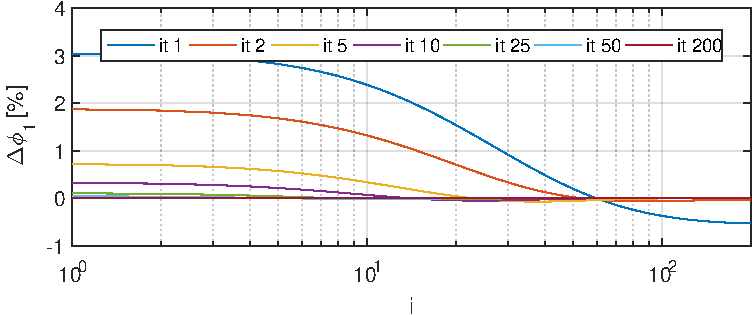
\includegraphics[width=0.45\linewidth]{flux_deviation_half_it_1.pdf}
%DIFDELCMD < 	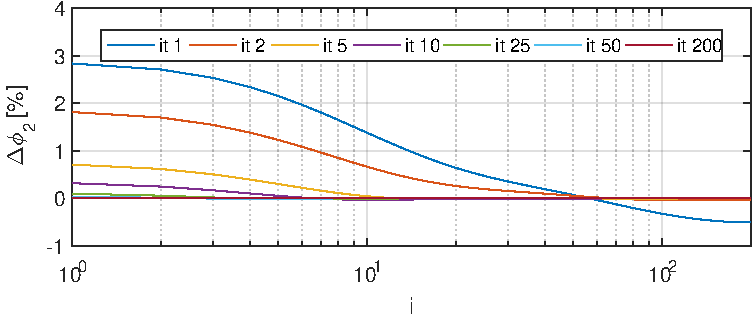
\includegraphics[width=0.45\linewidth]{flux_deviation_half_it_2.pdf}
%DIFDELCMD < 	%%%
\DIFdelendFL \DIFaddbeginFL 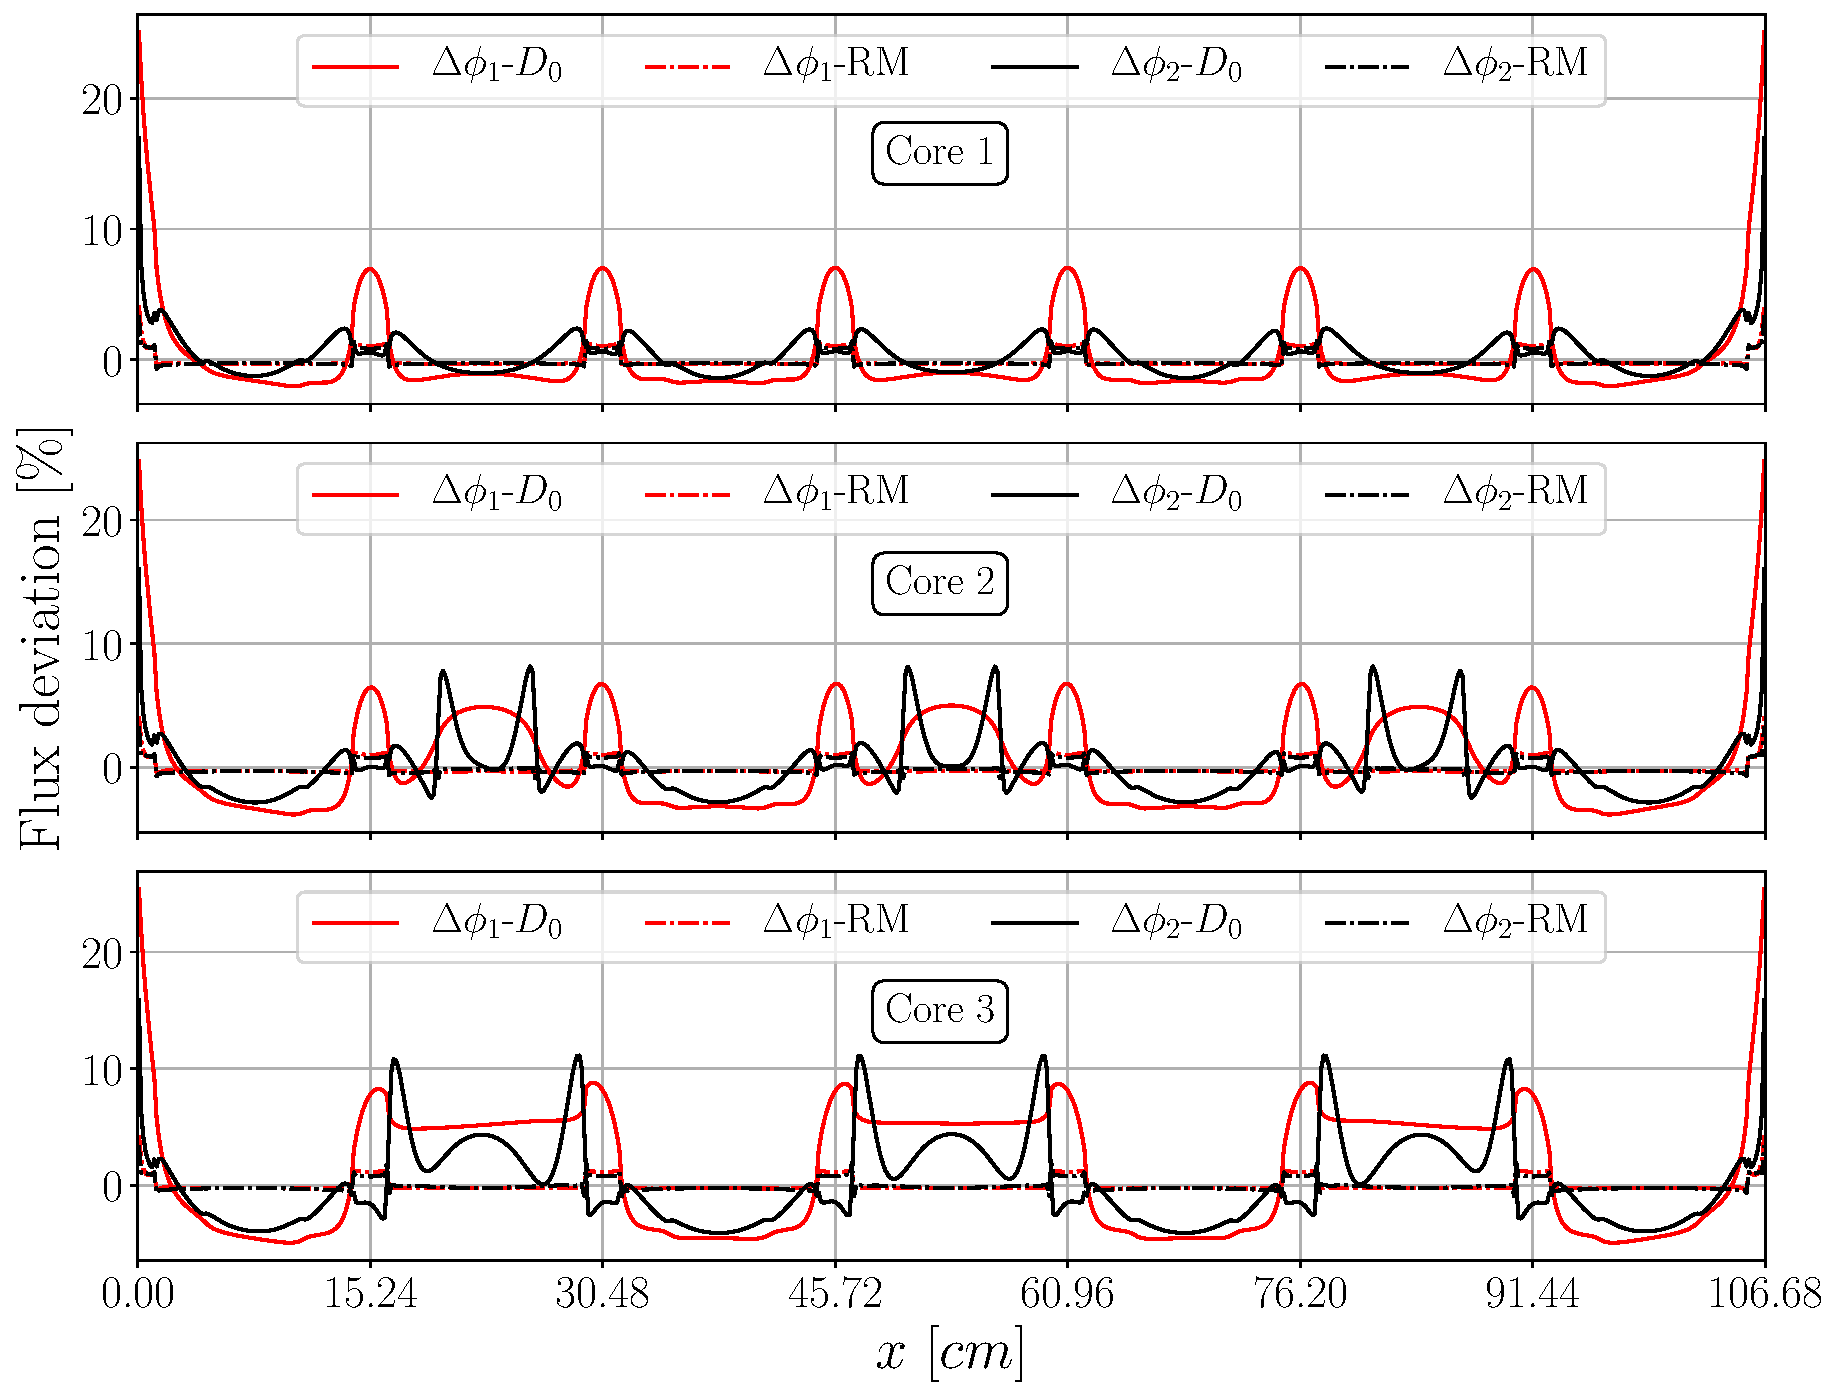
\includegraphics[width=0.75\linewidth]{flx_err_diff_C123.pdf}
	\DIFaddendFL \caption{\DIFdelbeginFL \DIFdelFL{The spatial }\DIFdelendFL \DIFaddbeginFL \DIFaddFL{Fast and thermal }\DIFaddendFL flux \DIFdelbeginFL \DIFdelFL{convergence between two successive }\DIFdelendFL \DIFaddbeginFL \DIFaddFL{deviation of standard diffusion ($D_0$) and }\DIFaddendFL Ronen \DIFdelbeginFL \DIFdelFL{iterations }\DIFdelendFL \DIFaddbeginFL \DIFaddFL{method (RM) with respect to S$_{16}$ reference solutions }\DIFaddendFL for \DIFaddbeginFL \DIFaddFL{each core. Vertical grid lines are located at assemblies interfaces. RM results are for 100 iterations and }\DIFaddendFL the \DIFdelbeginFL \DIFdelFL{left half slab, according to $\Delta\phi = (\phi^{k-1}-\phi^k)/\phi^{k-1}$ }%DIFDELCMD < [%%%
\DIFdelFL{\%}%DIFDELCMD < ]%%%
\DIFdelendFL \DIFaddbeginFL \DIFaddFL{spatial mesh spans 8 nodes in the water and 22 nodes in each fuel element}\DIFaddendFL .}
	\DIFdelbeginFL %DIFDELCMD < \label{fig:conv2}
%DIFDELCMD < %%%
\DIFdelendFL \DIFaddbeginFL \label{fig:hetero-flux-dev}
\DIFaddendFL \end{figure}

%DIF <  convergence
\DIFdelbegin %DIFDELCMD < \begin{figure}[htbp!]
%DIFDELCMD < 	%%%
\DIFdelendFL \DIFaddbeginFL \DIFaddFL{It is illustrative to examine the spatial distribution of the Ronen method correction factors for the heterogeneous case. The behavior of the correction factor (Fig.~\ref{fig:Dcoef}) may seem a bit erratic, but can be explained. In regions where the flux gradients are small, the correction factors tend to vanish and actually produce solutions similar to standard diffusion. However, in regions where the flux gradients are steep, the correction factors do not vanish and play an important role in reproducing the correct flux shape.
}

\begin{figure}[htbp]
	\DIFaddendFL \centering
	\DIFdelbeginFL %DIFDELCMD < 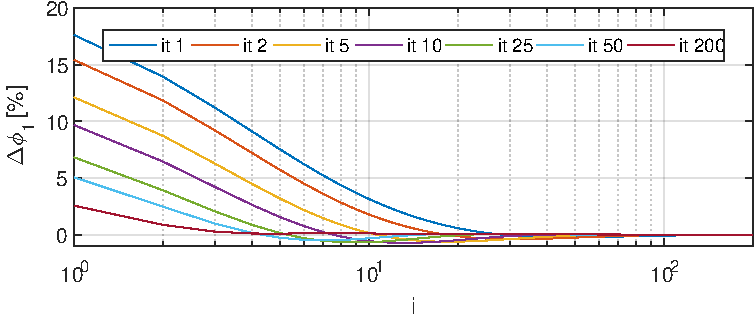
\includegraphics[width=0.45\linewidth]{flux_deviation_half_it_1_sn.pdf}
%DIFDELCMD < 	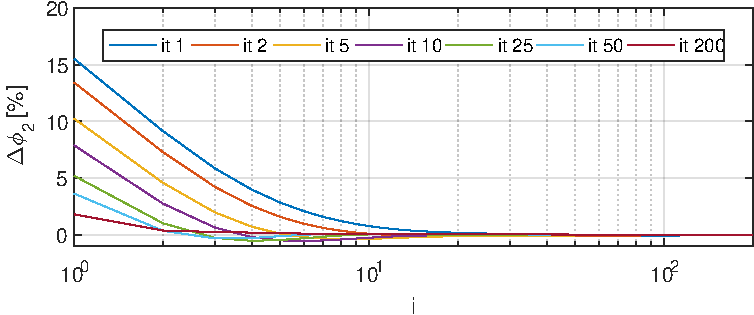
\includegraphics[width=0.45\linewidth]{flux_deviation_half_it_2_sn.pdf}
%DIFDELCMD < 	%%%
\DIFdelendFL \DIFaddbeginFL 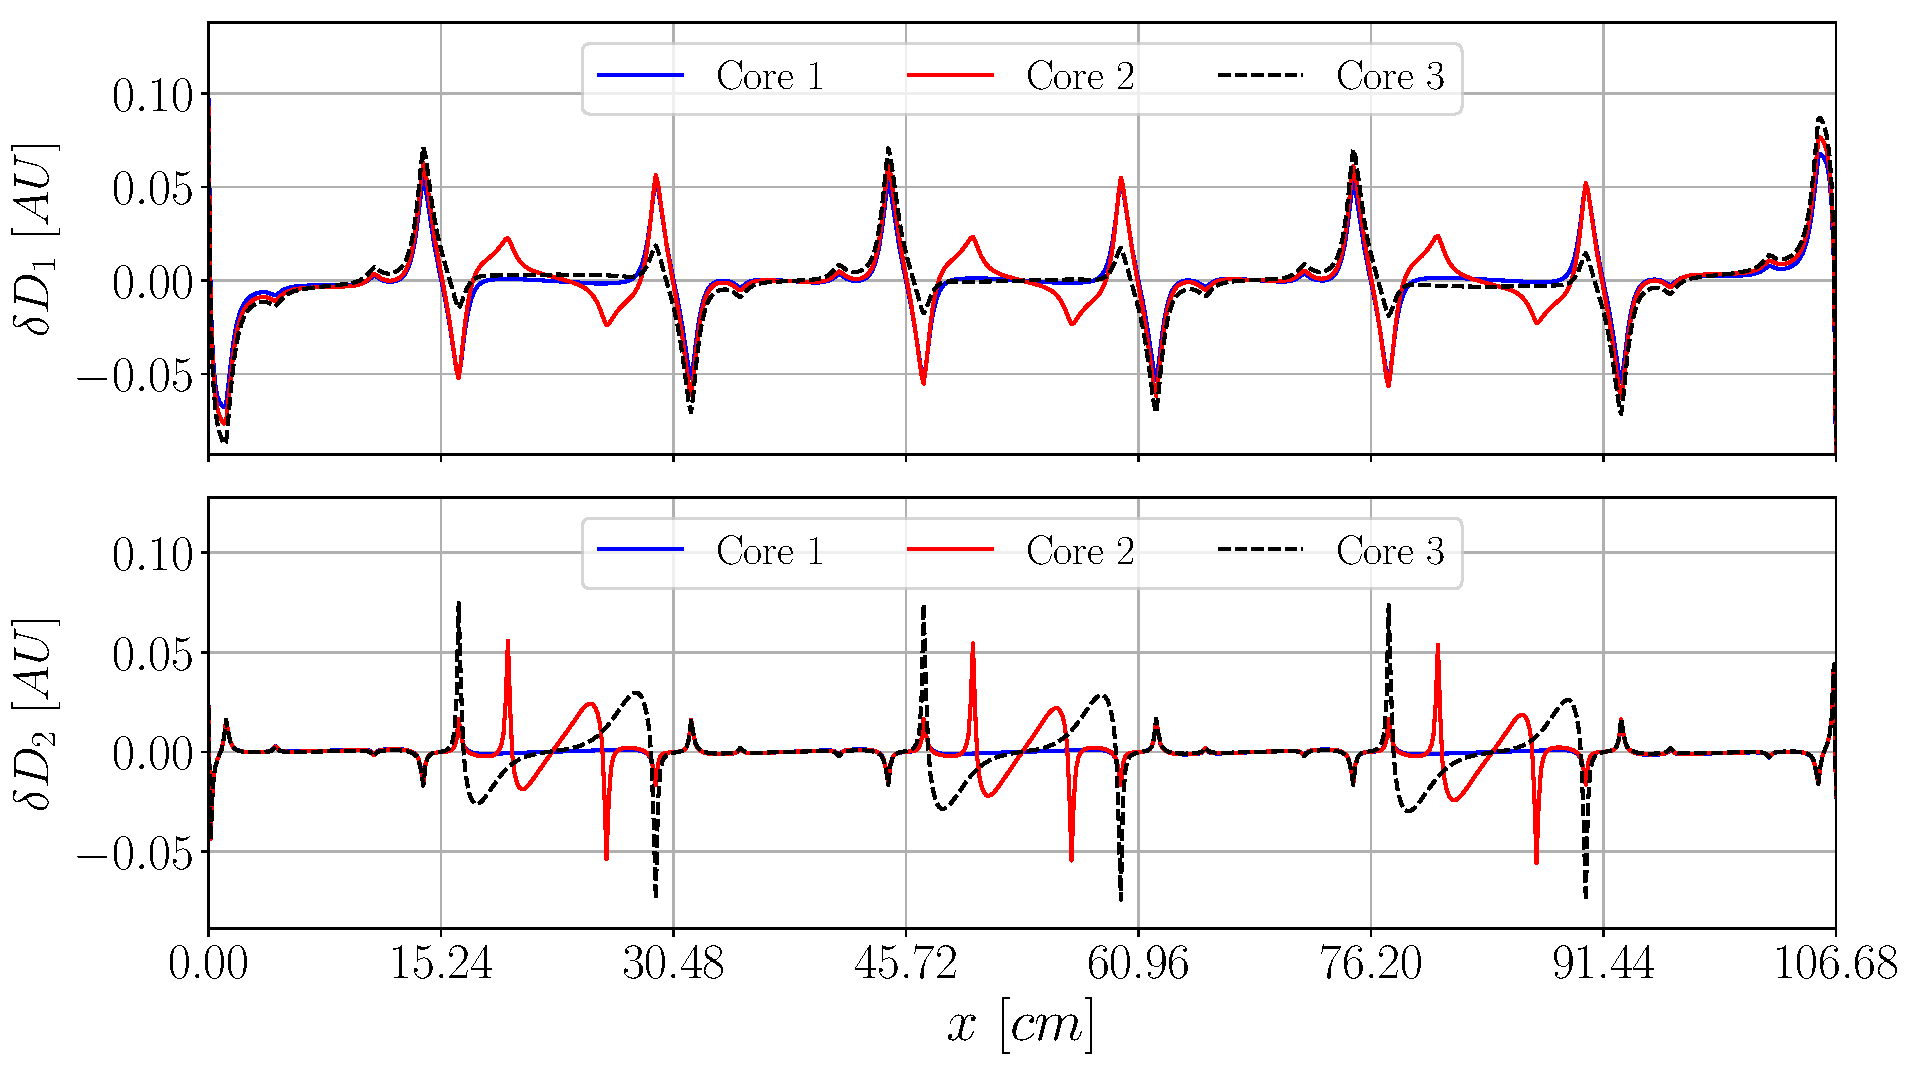
\includegraphics[width=0.75\linewidth]{RM_dD_100it_8_22_728_C123.pdf}
	\DIFaddendFL \caption{\DIFdelbeginFL \DIFdelFL{The spatial flux convergence }\DIFdelendFL \DIFaddbeginFL \DIFaddFL{Behavior }\DIFaddendFL of the Ronen \DIFdelbeginFL \DIFdelFL{iterations with respect to }\DIFdelendFL \DIFaddbeginFL \DIFaddFL{method correction factor $\delta D$ along }\DIFaddendFL the \DIFdelbeginFL \DIFdelFL{reference $S_n$ solution }\DIFdelendFL \DIFaddbeginFL \DIFaddFL{core, }\DIFaddendFL for the \DIFdelbeginFL \DIFdelFL{left half slab}\DIFdelendFL \DIFaddbeginFL \DIFaddFL{fast and thermal fluxes}\DIFaddendFL . \DIFaddbeginFL \DIFaddFL{Vertical grid lines are located at assemblies interfaces, results are for 100 iterations and the spatial mesh spans 8 nodes in the water and 22 nodes in each fuel element.}\DIFaddendFL }
	\DIFdelbeginFL %DIFDELCMD < \label{fig:conv3}
%DIFDELCMD < %%%
\DIFdelendFL \DIFaddbeginFL \label{fig:Dcoef}
\DIFaddendFL \end{figure}

%
% ---------------------------------------------------
\section{Conclusions}
\label{sec:conc}

The Ronen Method was first proposed for better estimates of the diffusion coefficient by calculating the current with a higher-order transport operator and a known best-estimate neutron flux. This yielded an iterative scheme leading to new flux distributions solved by a diffusion solver but with \DIFdelbegin \DIFdel{a }\DIFdelend \DIFaddbegin \DIFadd{additional }\DIFaddend (spatially) \DIFdelbegin \DIFdel{modified diffusion coefficient }\DIFdelend \DIFaddbegin \DIFadd{corrected diffusion terms, }\DIFaddend driving the diffusion solution to that of the integral transport equation. \DIFdelbegin \DIFdel{The direct resolution of the integral equation would imply the inversion of large matrices, with poor control of their conditioning. The solution of the diffusion equation, on the other hand, offers many numerical advantages, e.
g., speed and robustness. Nonetheless, }\DIFdelend %DIF > However, the direct resolution of the integral equation would imply the inversion of large matrices, with poor control of their conditioning. The solution of the diffusion equation, on the other hand, offers many numerical advantages, e.g., speed and robustness. 
\DIFaddbegin 

\DIFadd{The basic relation proposed by Ronen, i.e., Eq.~}\eqref{eq:RM-it-1D-slab}\DIFadd{, becomes problematic in the regions where the gradient of the flux is small, that is usually where diffusion performs well. Ronen did not elaborate on this issue in his technical note from 2004. Theoretically, both the numerator and the denominator should vanish at the same location since both are accurate expressions for the neutron current with weak flux gradients. We assume that this ratio, considered as a ratio between two quantities which tend to zero at the same location, approaches some constant value since there exist a diffusion coefficient at that location. However, any value would be possible in Fick's law because of the vanishing flux grandient.
}

\DIFadd{Numerically, Tomatis and Dall'Osso chose in 2011 to deal with this potential singularity by using the well-known drift terms, which serve as a }\emph{\DIFadd{numerical feature}}\DIFadd{. The (more accurate) surface current $\jtrr$, calculated by the integral expression, is written as the sum of the surface current calculated by diffusion, $\jd$, plus a correction $\delj$. Hence, when the current vanishes, }\DIFaddend the \DIFdelbegin \DIFdel{same current can be enforced in the discretized form of the diffusion equation as suggested by the CMFD, which avoids the numerical issues resulting from small flux gradients. This is the option adopted in this study.}\DIFdelend \DIFaddbegin \DIFadd{correction $\delj$ vanishes as well. Moreover, the correction is written as in Eq.~}\eqref{eq:dJ}\DIFadd{, avoiding the potential divergence resulting from division by zero.
}\DIFaddend 

%DIF > Nonetheless, the same current can be enforced in the discretized form of the diffusion equation as suggested by the CMFD, which avoids the numerical issues resulting from small flux gradients. This is the option adopted in this study.  
\DIFaddbegin 

\DIFaddend More accurate results are obtained for the two-group benchmark problem reported in \cite{Tomatis-2011} \DIFdelbegin \DIFdel{. }\DIFdelend \DIFaddbegin \DIFadd{and new results are reported for a heterogeneous benchmark. The performances of the Ronen method, especially for the heterogeneous benchmark (as shown in Figs.~\ref{fig:hetero-flux}--\ref{fig:Dcoef}), strongly indicate that it is inherently suitable to deal with non-homogeneous systems and can naturally adapt to interfaces, where strong gradients of the flux might appear.
}

\DIFaddend In general, slow convergence is observed for the scalar flux \DIFdelbegin \DIFdel{, whose larger discrepancy with respect }\DIFdelend \DIFaddbegin \DIFadd{with the larger discrepancies, comparing }\DIFaddend to the reference\DIFdelbegin \DIFdel{is always }\DIFdelend \DIFaddbegin \DIFadd{, }\DIFaddend located on the vacuum boundary \DIFaddbegin \DIFadd{and on the material interfaces}\DIFaddend . Although the method is converging to the reference results provided by a discrete ordinate transport code, the improvement of the convergence rate and the use of coarser meshes are crucial for the advancement of the methodology in practical applications. These topics will be addressed as future developments, as well as \DIFdelbegin \DIFdel{heterogeneous systems and }\DIFdelend higher-order anisotropy.

%
% ---------------------------------------------------
\section*{Acknowledgments}
\label{sec:acknow}
\DIFdelbegin %DIFDELCMD < 

%DIFDELCMD < %%%
\DIFdelend The authors express their gratitude to Prof. Yigal Ronen who initiated the idea for this study. R.G. is partially supported by the Israel Ministry of Energy, contract no. 216-11-008. 


%\appendix
%\section{Test 1}
%sdf asd asd adsf 
%\section{Test 2}
%sdf sdf sd


%
% BibTeX users please use
\bibliographystyle{unsrt}
\bibliography{refs-EPJP}

\end{document}
